\documentclass[a4paper,12pt]{book}

\usepackage[utf8]{inputenc}
\usepackage[spanish]{babel}
%\usepackage{listings}
\usepackage{graphicx}

\usepackage{color}
\definecolor{gray97}{gray}{.97}
\definecolor{gray75}{gray}{.75}
\definecolor{gray45}{gray}{.45}

\usepackage{listings}
\lstset{ frame=Ltb,
framerule=0pt,
aboveskip=0.5cm,
framextopmargin=3pt,
framexbottommargin=3pt,
framexleftmargin=0.4cm,
framesep=0pt,
rulesep=.4pt,
backgroundcolor=\color{gray97},
rulesepcolor=\color{black},
%
stringstyle=\ttfamily,
showstringspaces = false,
basicstyle=\small\ttfamily,
commentstyle=\color{gray45},
keywordstyle=\bfseries,
%
numbers=left,
numbersep=15pt,
numberstyle=\tiny,
numberfirstline = false,
breaklines=true,
}

% minimizar fragmentado de listados
\lstnewenvironment{listing}[1][]
{\lstset{#1}\pagebreak[0]}{\pagebreak[0]}

% estilo para poner comandos de consola
\lstdefinestyle{consola}
{basicstyle=\scriptsize\bf\ttfamily,
backgroundcolor=\color{gray75},
}

% estilo para código Java
\lstdefinestyle{Java}
{language=Java,
}





\title{\Huge Plataforma de firma digital para la Universidad de Málaga.}
	
 	\author{Juan Antonio Pérez Ariza \\
		Escuela Técnica Superior Ingeniería Informática \\
		Universidad de Málaga \\
		\\
		Profesor: \\
		Isaac Agudo Ruíz\\
		Departamento Lenguajes y Ciencias de la Comunicación \\
		Universidad de Málaga}

\begin{document}
	\maketitle	
	
	%Table of contents	
	\tableofcontents
	
	%separacion entre parrafos
	\parskip=5mm
	
	\mainmatter
	%introducción
	\chapter{Introducción.}
En este primer capítulo de la memoria vamos a explicar las motivaciones que nos llevaron a pensar en realizar dicho proyecto, los objetivos que nos marcamos cuando lo diseñamos, los materiales usados y la organización de esta memoria.

\section{¿Por qué decidimos hacer el proyecto?}
Al igual que muchos estudiantes de la Universidad de Málaga, yo suelo comer habitualmente en la cafetería de la facultad y hay mucha personas que se molesta cuando le piden que firme el papel con el que se lleva el recuento de los estudiantes que comen en las cafeterías para el descuento por ser estudiante. Además de este inconveniente hay un par de problemas más, que son lo molesto que es tener que firmar todos los días o habitualmente y las colas que se forman al tener que rellenar el nombre y la firma, por eso se decidió hacer una aplicación para terminales móviles con la que agilizar todo este proceso de firma y control de estudiantes, mediante la lectura de un código QR que tendría la información necesaria para la realización de la firma.

A medida que avanzaba el proyecto se vio que se podía ampliar la funcionalidad de la aplicación, no solo al comedor, si no también a alquiler de pistas o cualquier documento necesario en la Universidad de Málaga.

Otra razón para la realización de este proyecto es que a mi me gusta la seguridad informática y vi en este proyecto una buena forma de aprender más sobre criptografía, particularmente en la criptografía de clave pública. También vi una buena forma de aprender a programar para terminales Android, debido al gran auge que tienen en este momento los terminales móviles, y a crear aplicaciones web de las que no tenía ninguna idea. Al inicio la aplicación web se pensó en hacer directamente en java sin ninguna ayuda, pero se descartó ante la dificultad de encontrar un servicio de hosting gratuito, por lo que se decidió cambiar a una sugerencia que hizo director de proyecto de usar una plataforma que proporciona Google llamada Google App Engine, que es gratuita y se pueden crear aplicaciones web programadas en el lenguaje de programación Java y así tener la posibilidad de aprender otras APIS, no solo Java2EE.

\section{Objetivos que queríamos conseguir.}

El principal objetivo que queríamos conseguir era que la forma de firmar fuera muy fácil y que no fuera un mecanismo muy engorroso. Para ellos decidimos realizar una aplicación para smartphone Android y una aplicación web para el almacenamiento y posterior comprobación de las firmas.

Una vez teníamos clara la idea, empezamos a diseñar un sistema con el que se pudiera realizar la firma digital inicialmente, solo de un recibo y finalmente cualquier documento de la UMA agilizando de esta forma dicho proceso.

%TODO: Hay poner algo de criptografía... xDDD

En la parte de la aplicación de Android se decidió hacer una aplicación clara y que fuese fácil de usar. Para eso usamos la API nivel 14 que equivale a la versión 4.0 de Android, llamada Ice Cream Sandwich. Se eligió porque proporciona una nueva forma de diseño de las interfaces, un nuevo tema  llamado Holo y proporciona muchas nuevas herramientas como por ejemplo son los ActionBar, que es una barra que permanece siempre en la parte superior de la pantalla, la que se va acomodando a las necesidades que tiene la aplicación cambiando los botones con diferentes funcionalidades, por ejemplo si estamos en la pantalla principal pues tendremos siempre visible el botón de añadir un nuevos recibo que abrirá el lector de códigos QR, se puede observar en la primera barra de la figura~\ref{fig:actionBar}, sin embargo si estamos visualizando un recibo solo tendremos el botón de volver atrás, como se puede ver en la segunda barra de la figura~\ref{fig:actionBar}, en la que se puede ver que al lado del icono de la aplicación una flechita que indica que es el botón para volver atrás.

\begin{figure}
  \centering
    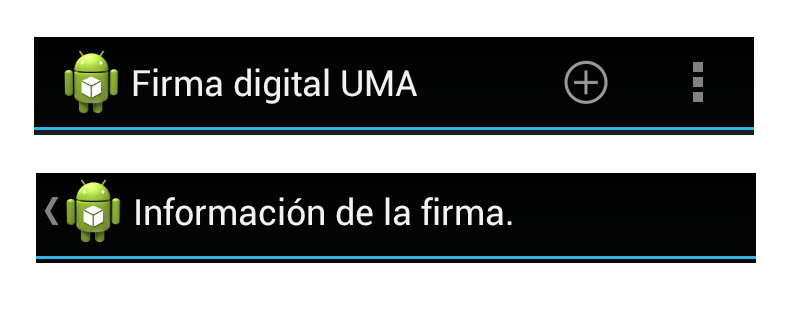
\includegraphics[scale=0.3]{./Introduccion/imagenes/actionbar.png}
  \caption{Action Bar.}
  \label{fig:actionBar}
\end{figure}

Al tomar la decisión de programar para terminales con Android 4.0 o mayor estuvimos sopesando los pros y los contras, y al final decidimos que la implantación de Android 4.0 cada vez es mayor y que cada día hay más terminales con dicha versión, como se puede ver en este gráfico de la figura~\ref{fig:graficoEvolucionAndroid} y podemos observar que a finales de agosto de este año la cantidad de usuarios afectados sería de más del 15\% de terminales como podemos ver en la figura~\ref{fig:graficoUsoAndroid}, aunque todavía sigue reinando la versión 2.3.3, aunque creemos que el cambio a la versión 4.0 o superior será rápida debido a todas las ventajas que aporta y mucho más ahora que hace unos meses Google sacó una nueva versión, la 4.1, llamada Jelly Bean y casi todas las compañías querrán actualizar sus terminales a la última versión, por lo que a pesar de dejar a un gran número de usuarios sin poder usar la aplicación preferimos funcionalidad y elegancia frente a gran cantidad de usuarios, ya que estos llegarán a medida que sus compañías actualicen sus terminales.


\begin{figure}
  \centering
    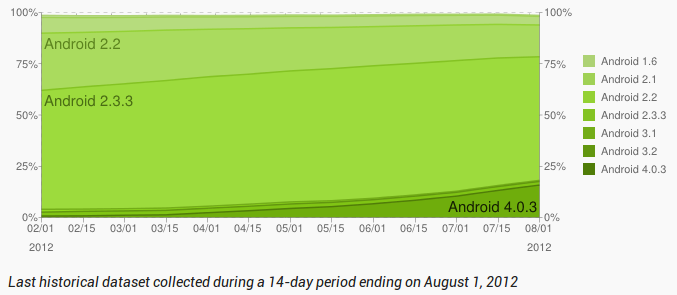
\includegraphics[scale=0.8]{./Introduccion/imagenes/graficoEvolucionAndroid.png}
  \caption{Gráfico de las versiones de Android a principio de octubre del 2012.}
  \label{fig:graficoEvolucionAndroid}
\end{figure}

\begin{figure}
  \centering
    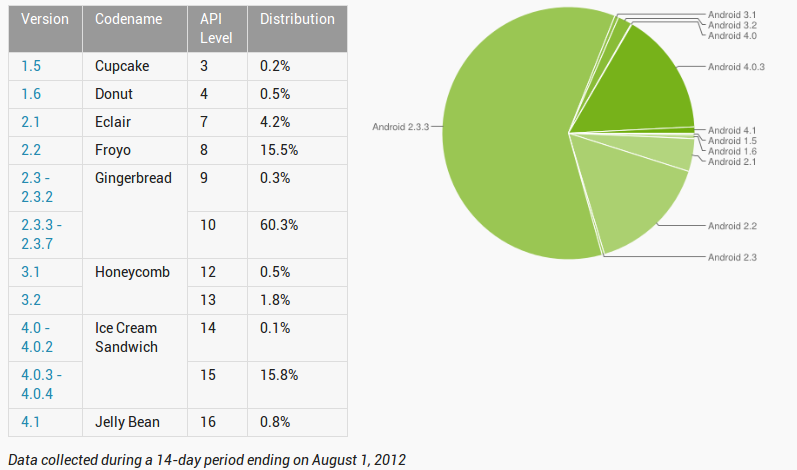
\includegraphics[scale=0.5]{./Introduccion/imagenes/graficoUsoAndroid.png}
  \caption{Gráfico del uso de las versiones de Android a principios de octubre del 2012.}
  \label{fig:graficoUsoAndroid}
\end{figure}

En la parte del servidor al elegir la plataforma de Google, hubo muchas cosas que resultaron más fáciles a costa de tener que aprender a usar el SDK que Google proporciona, que como era una de las cosas por la que elegimos dicha plataforma no nos importó. Una de las cosas que nos facilitaba es la gestión de usuarios, que los gestiona Google directamente al tener que usar una cuenta de Google Account para usar la aplicación web. Toda la seguridad y mantenimiento de los servidores, copias de seguridad, balanceos de carga y otra gran cantidad de funciones también las realiza Google, por lo que nos eximen de su realización y no tendremos que preocuparnos de ellas.

\section{Organización de la memoria.}

En el primer capítulo, que es el actual, hemos realizado una introducción al proyecto, explicado la idea inicial y los materiales usados. Para continuar en el capítulo segundo de la memoria explicaremos los conocimientos básicos sobre todas las tecnologías usadas en el proyecto, como pueden ser Android, Java, criptografía, HTML, GIT, etc. En el tercer capítulo hemos hecho una breve introducción a la criptografía que hemos usado a lo largo del proyecto, centrándonos más en la criptografía de clave pública, RSA y como usarla con el lenguaje de programación Java. En el capítulo cuarto, explicaremos los conocimientos básicos necesarios para entender Android y Google App Engine, explicamos los archivos que se usan en ambos proyectos y las características principales de cada arquitectura. En el capítulo quinto es el principal de la memoria, en él se explica la arquitectura diseñada para el proyecto, la metodología usada y la implementación tanto la aplicación móvil en Android como de ambas aplicaciones web. En el último capítulo tendremos el desenlace del proyecto en el que expondremos las conclusiones, problemas y posibles trabajos futuros que hemos observado que se podrían realizar. Para finalizar tendremos tres anexos en los que explicaremos la configuración de la plataforma Eclipse para el uso de la API Google App Engine como la de Android, la creación de los certificados de clave pública y el contenido del CD.  

\section{Material usado.}
Para la realización del proyecto hemos usado un ordenador personal para todo el proceso de programación y un smartphone con Android para la depuración y prueba de la aplicación. 

El ordenador es un ordenador portátil, con Ubuntu 12.04 como sistema operativo, un procesador Pentium Dual Core a 2.2Ghz, 4 Gb de memoria ram.

El móvil usado es un Samsung Galaxy Nexus (figura~\ref{fig:nexus}) que fue el móvil presentado cuando Google lanzó la versión 4.0, por lo que es el primer terminal en usar Android 4.0 y meses después el primero en recibir la actualización de Android 4.1. Sus característica son una pantalla de 4.65 pulgadas Super Amoled con resolución de 1280 x 720, procesador dual-core a 1.2Ghz, HSPA+, NFC, Wifi, GPS, etc.

\begin{figure}
  \centering
    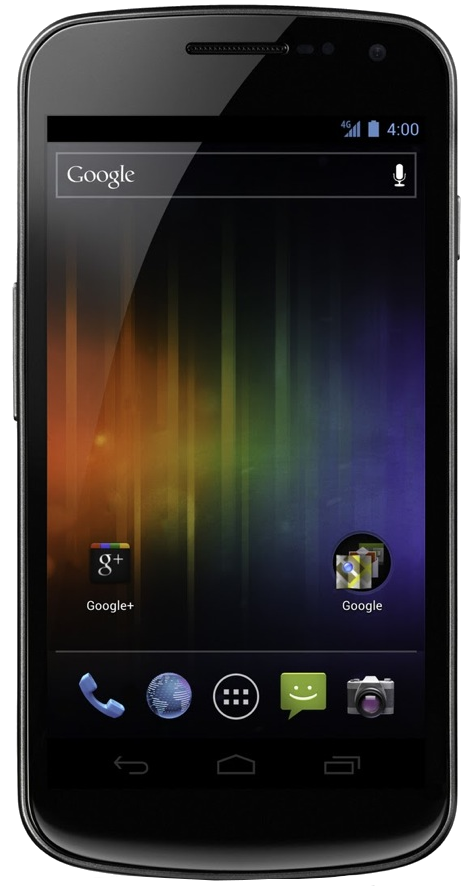
\includegraphics[scale=0.3]{./Introduccion/imagenes/nexus.png}
  \caption{Samsung Galaxy Nexus.}
  \label{fig:nexus}
\end{figure}

No tenemos datos sobre las máquinas usadas por los servidores donde Google da el servicio de Google App Engine.


	%conocimientos previos sobre las tecnologías
	\chapter[Conocimientos previos]{Conocimientos previos sobre las tecnologías usadas.}\label{cap:conocimientos}

En este segundo capítulo vamos a explicar cuales son y los conocimientos que poseíamos sobre las tecnologías que hemos usado en el proyecto. Haciendo una breve explicación sobre su funcionamiento, su uso, su historia y sus recientes versiones.

El principal elemento usado en el proyecto es el lenguaje de programación Java, que lo hemos usado para programar tanto la aplicación web como la aplicación en el móvil. Pero a parte de los diferentes SDK de Android y de Google App Engine, nos han hecho falta muchas otras tecnologías y lenguajes como pueden ser SQL, XML, UML, GIT. Además de los conocimientos básicos sobre criptografía de clave pública necesarios para realizar todo el proceso de firma digital.   

\section{El lenguaje de programación Java}

Java es un lenguaje de programación orientado a objetos que fue diseñado por Jame Gosling\footnote{Para más información sobre Jame Gosling: \url{http://en.wikipedia.org/wiki/James\_Gosling}} para Sun Microsystems y que recientemente ha sido comprada por Oracle Corporation. Fue lanzado en 1995 y fue el centro de toda la plataforma Java de Sun Microsystems. Es un lenguaje con una sintaxis muy parecida a C o C++, pero con la gran ventaja de que el manejo de punteros y objetos es automático, al igual que la recogida de basura.

Java es un lenguaje en el que hay que compilar los código fuentes para crear unos archivos intermedios llamados bytecodes, los archivos *.class, que luego serán interpretados por la máquina virtual de Java (JVM). Esta dependerá de la arquitectura en la que se quiera ejecutar la aplicación Java. Gracias a esto se puede decir que Java es un lenguaje multiplataforma, lo que significa que un mismo código Java se puede ejecutar en Linux, en Windows, un Mac o cualquier otro sistema para el cual exista una máquina virtual, lo que en inglés se llama "write once, run anywhere" (WORA). Además de esta importante ventaja Java es un lenguaje de propósito general, concurrente, basado en clases y orientado a objetos. Java es el segundo lenguaje de programación más popular de 2012, gracias a las aplicaciones web cliente-servidor que tienen tanto auge en estos momentos, como podemos ver en la figura \ref{fig:indicetiobe}.

\begin{figure}[h]
  \centering
    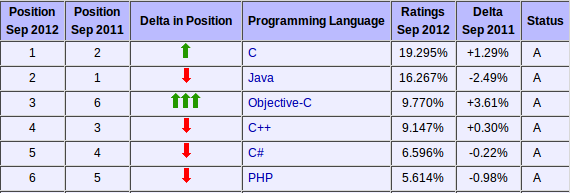
\includegraphics[scale=0.9]{./ConocimientosPrevios/imagenes/indiceTiobe.png}
  \caption{Índice tiobe en septiembre del 2012. \url{http://www.tiobe.com/}}
  \label{fig:indicetiobe}
\end{figure} 

La implementación original y las referencias del compilador de Java, máquinas virtuales y las librerías de clases fueron desarrollado por Sun en 1995, pero en el 2007 gracias a la contribución de la comunidad, Sun Microsystem cambió la licencia de todas las tecnologías Java a GNU General Public License, por lo que se abría la posibilidad a que se crearan versiones alternativas de compiladores bajo licencia GNU como por ejemplo GNU Compiler para Java o GNU Classpath.

En el proyecto la versión usada fue la versión \textbf{Java SE}.

\subsection{Historia}

Originalmente Java nació como un proyecto de James Gosling, Mike Sheridan, and Patrick Naughton en 1991 y estaba diseñado para una televisión interactiva, pero era muy avanzado para lo que la industria televisiva de la época podía necesitar. En su origen fue llamado como Oak, pero por problemas con el nombre, ya que era una marca registrada de otra empresa, lo cambiaron a Green y posteriormente ya lo renombraron al definitivo Java. Hay muchas teorías sobre el porque se llama Java, pero una de ellas es que había una cafetería llamada Java Coffe donde Jame, Mike and Patrick pasaron muchas horas consumiendo café.

La idea de Gosling era crear una máquina virtual donde funcionara un lenguaje de programación con la sintaxis y la estructura de C/C++ para que la curva de aprendizaje fuera muy suave a los programadores que en la época sabían C/C++.

Sun Microsystem lanzó Java 1.0 en 1995, con la principal característica de que una vez escrito un código fuente no había que modificarlo para que funcionara en las diferentes máquinas, lo que anteriormente hemos llamado con el acrónimos en inglés WORA (Write Once, Run Anywhere). Rápidamente todos los navegadores de la época empezaron a soportar applet Java en las páginas web, por lo que Java se volvió muy popular en la época. La nueva versión Java 2 fue lanzada en 1998-1999 y con ella llegaron las distinciones en diferentes plataformas, como por ejemplo Java2EE para aplicaciones corporativas o una versión ligera llamada Java2ME que estaba diseñada para funcionar en los diferentes teléfonos de la época, y el resto se agrupan en la versión Java2SE, que es la versión estándar.

En 1997, Sun Microsystem intentó formalizar Java mediante una norma ISO/IEC pero se retiró del proceso y dio todo el control a la comunidad. Sun ofrecia implementaciones gratuitas y generaba dinero vendiendo algunas licencias de productos como Java Enterprise System. Una cosa importante es que Sun distingue entre el SDK (Kit de desarrollo) y el JRE (Entorno de ejecución) en el que van incluidos los compiladores, debugger, etc.

El 13 de noviembre del 2006, Sun lanzó Java gratis y software libre, bajo la licencia GNU General Public License (GPL). El proceso finalizó el 8 de mayo del 2007.

En 2009-2010 Oracle Corporation compró Sun Microsystem por lo que Java actualmente pertenece a Oracle Corporation.

\subsection{Versiones}

\begin{itemize}

	\item \textbf{JDK 1.0} (23 de enero de 1996): Primer lanzamiento
	
	\item \textbf{JDK 1.1} (19 de febrero de 1997): Las primeras características añadidas fuero una reestructuración intensiva del modelo de eventos AWT (Abstract Windowing Toolkit), clases internas (inner classes), JavaBeans, JDBC (Java Database Connectivity), para la integración de bases de datos y RMI (Remote Method Invocation).
	
     \item \textbf{JDK 1.2}(8 de diciembre de 1998): Recibió el nombre en clave Playground. Esta y las siguientes versiones fueron recogidas bajo la denominación Java 2 y el nombre "J2SE" (Java 2 Platform, Standard Edition), reemplazó a JDK para distinguir la plataforma base de J2EE (Java 2 Platform, Enterprise Edition) y J2ME (Java 2 Platform, Micro Edition). 
    Se añadieron las siguientes mejoras, la palabra reservada strictfp, reflexión en la programación, la API gráfica ( Swing) fue integrada en las clases básicas, la máquina virtual (JVM) de Sun fue equipada con un compilador JIT (Just in Time) por primera vez, Java Plug-in, Java IDL, una implementación de IDL (Lenguaje de Descripción de Interfaz) para la interoperabilidad con CORBA y Colecciones.

    \item \textbf{J2SE 1.3} (8 de mayo de 2000): Recibió el nombre en clave Kestrel. Los cambios más notables fueron: la inclusión de la máquina virtual de HotSpot JVM, RMI fue cambiado para que se basara en CORBA, JavaSound, se incluyó el Java Naming and Directory Interface (JNDI) en el paquete de bibliotecas principales (anteriormente disponible como una extensión), Java Platform Debugger Architecture (JPDA).

    \item \textbf{J2SE 1.4} (6 de febrero de 2002): Recibió el nombre en clave Merlin. Este fue el primer lanzamiento de la plataforma Java desarrollado bajo el Proceso de la Comunidad Java como JSR 59. Las principales características que se le añadieron fueron palabra reservada assert, expresiones regulares modeladas al estilo de las expresiones regulares Perl, encadenación de excepciones, non-blocking NIO (New Input/Output), logging API, API I/O para la lectura y escritura de imágenes en formatos como JPEG o PNG, parser XML integrado y procesador XSLT (JAXP), seguridad integrada y extensiones criptográficas (JCE, JSSE, JAAS), Java Web Start incluido.
    
    \item \textbf{J2SE 5.0} (30 de septiembre de 2004): Recibió el nombre en clave Tiger. Estos fueron los cambios mas importantes, plantillas (genéricos), metadatos, también llamados anotaciones, permite a estructuras del lenguaje como las clases o los métodos, ser etiquetados con datos adicionales, que puedan ser procesados posteriormente por utilidades de proceso de metadatos, autoboxing/unboxing, conversiones automáticas entre tipos primitivos (Como los int) y clases de envoltura primitivas (Como Integer), enumeraciones, varargs (número de argumentos variable), el último parámetro de un método puede ser declarado con el nombre del tipo seguido por tres puntos (por ejemplo \lstinline{void drawtext(String... lines)}). En la llamada al método, puede usarse cualquier número de parámetros de ese tipo, que serán almacenados en un array para pasarlos al método, bucle for mejorado, La sintaxis para el bucle for se ha extendido con una sintaxis especial para iterar sobre cada miembro de un array o sobre cualquier clase que implemente Iterable, como la clase estándar Collection, de la siguiente forma:

\begin{lstlisting}[style=Java]
void displayWidgets (Iterable<Widget> widgets) {
	for (Widget w : widgets) {
		w.display();
	}
}
\end{lstlisting}

    \item \textbf{Java SE 6} (11 de diciembre de 2006): Recibió el nombre en clave Mustang. En esta versión, Sun cambió el nombre "J2SE" por Java SE y eliminó el ".0" del número de versión. Los cambios más importantes introducidos en esta versión fueron un nuevo marco de trabajo y APIs que hacen posible la combinación de Java con lenguajes dinámicos como PHP, Python, Ruby y JavaScript, el motor Rhino, de Mozilla, una implementación de Javascript en Java, un cliente completo de Servicios Web y soporta las últimas especificaciones para Servicios Web, mejoras en la interfaz gráfica y en el rendimiento.
    
    \item \textbf{Java SE 7}: Su nombre en clave es Dolphin. Su lanzamiento fue en julio de 2011. Y las principales nuevas características fuero: soporte para XML dentro del propio lenguaje, un nuevo concepto de superpaquete, soporte para closures, introducción de anotaciones estándar para detectar fallos en el software.

\end{itemize}

\section{El entorno de programación Eclipse.}

Eclipse es un entorno integral de desarrollo que consta de un entorno de desarrollo integrado (IDE) y es extensible mediante plugins que está escrito en Java. Puede ser usado para una larga lista de lenguajes de programación como pueden ser C, C++, Haskell, Perl, PHP, Python, Android y un largo etcétera. Fue originalmente desarrollado por IBM y fue lanzado con la licencia de software Eclipse Public License\footnote{Para más información visite: \url{http://en.wikipedia.org/wiki/Eclipse\_Public\_License}} la cual es una licencia de software libre. El SDK de Eclipse es libre y tiene licencia Open Source por lo que cualquier persona con los conocimientos necesarios puede programar el plugin que necesite para Eclipse. Fue el primer entorno de programación que funcionó bajo GNU Classpath y que funcionaba sin problemas con IcedTea. En la figura \ref{fig:pantallaEclipse} se puede ver el aspecto que tiene.

\begin{figure}
  \centering
    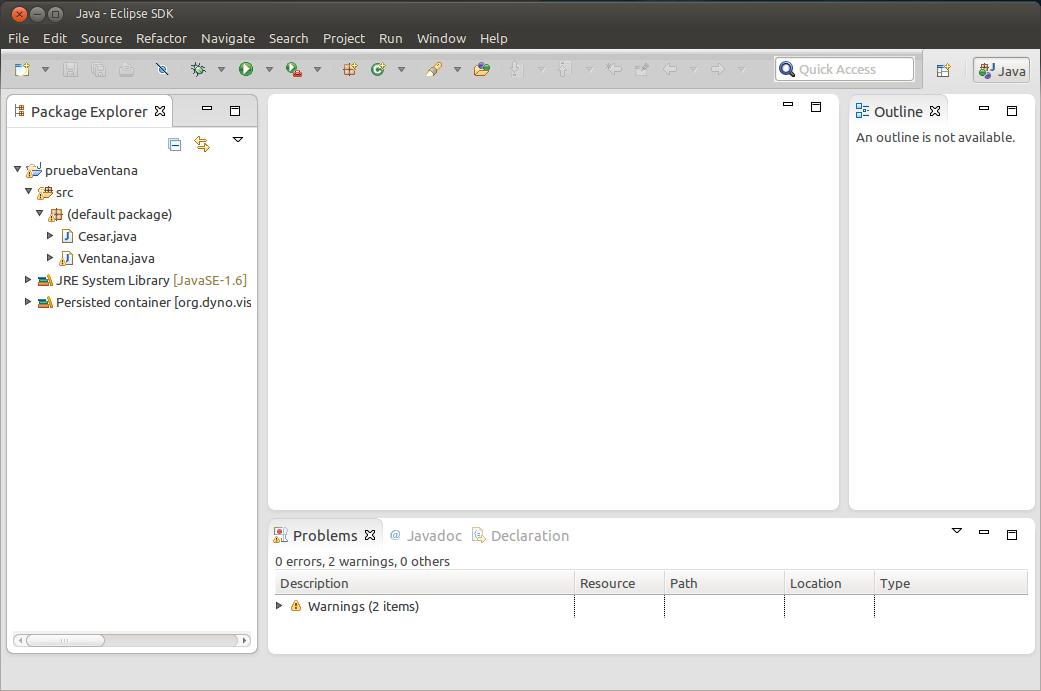
\includegraphics[scale=0.5]{./ConocimientosPrevios/imagenes/pantallaEclipse.png}
  \caption{Eclipse 4.2 Juno.}
  \label{fig:pantallaEclipse}
\end{figure} 

En el proyecto hemos usado la versión \textbf{Indigo}, que equivale a la versión 3.7 de Eclipse.

\subsection{Historia}

Eclipse comenzó como un proyecto de IBM Canadá. En noviembre de 2001 se creó un grupo de empresas para promover el desarrollo de Eclipse como software libre, los miembros iniciales eran Borland, IBM, Merant, QNX Software Systems, Rational Software, Red Hat, SuSE, TogetherSoft and WebGain. Finalmente en enero de 2004 se creó la Eclipse Foundation. 

\subsection{Versiones}

\begin{itemize}

	\item \textbf{Versión 3.0} (21 de junio de 2004)
	
	\item \textbf{Versión 3.1} (28 de junio de 2005)
	
	\item \textbf{Versión 3.2} (30 de junio de 2006): recibió el nombre de Callisto.
	
	\item \textbf{Versión 3.3} (29 de junio de 2007): recibió el nombre de Europa.
	
	\item \textbf{Versión 3.4} (25 de junio de 2008): recibió el nombre de Ganymede.
	
	\item \textbf{Versión 3.5} (24 de junio de 2009): recibió el nombre de Galileo.
	
	\item \textbf{Versión 3.6} (23 de junio de 2010): recibió el nombre de Helios.
	
	\item \textbf{Versión 3.7} (22 de junio de 2011): recibió el nombre de Indigo.
	
	\item \textbf{Versión 4.2} (27 de junio de 2012): recibió el nombre de Juno.
	
	\item \textbf{Versión 4.3} (26 de junio de 2013): esta será la próxima versión, que saldrá el próximo año y recibirá el nombre de Kepler.

\end{itemize}

\section{Criptografía.}\label{lbl:criptografia}

La criptografía es la ciencia que se encarga del estudio y creación de técnicas para la protección de una comunicación, para que solamente los usuarios autorizados pueda verla, leerla y entenderla. En la actualidad la criptografía es un término que se usa de forma similar a encriptación, que es el proceso para transformar una información mediante diferentes algoritmos, en un mensaje que no pueda entender un atacante que intercepte una comunicación. 

En el proyecto hemos usado una criptografía llamada \textbf{Criptografía de Clave Pública}, que como veremos a continuación en la historia brevemente y en el capítulo~\ref{cap:criptografia} en el que se explicará la criptografía usada en el proyecto, en profundidad, consta de dos claves, ambas enlazadas matemáticamente y si sabemos una no podremos de ninguna forma conseguir la otra. La pública  es la que tendría la persona que quiera desencriptar el mensaje, que a su vez da nombre a este algoritmo y otra privada que solo conocerá la persona que quiere encriptar el mensaje.

La criptografía ha evolucionado mucho y actualmente no solo se usan para proteger mensajes, si no que también se usa para proteger la integridad de ellos. Este es uno de los usos más común de la criptografía de clave pública.

\subsection{Historia}

Podemos hacer dos grandes grupos dentro de la historia de la criptografía, la criptografía clásica y la criptografía durante la época de los ordenadores.

\subsection{Criptografía clásica.}

	Durante la época de la criptografía clásica solo se quería proteger el mensaje que se enviaba de la mirada de curiosos y enemigos por lo que solo existían algoritmos de encriptación, la integridad del mensaje no importaba en esa época.  
	
	En dicha época todos los algoritmos de cifrados que existían eran por transposición o sustitución de caracteres. A continuación vamos a poner unos ejemplos de los algoritmos utilizados más famosos. 
\begin{itemize}

	\item \textbf{Cifrado Cesar:} dicho cifrado es famoso porque los usaban las centurias romanas para comunicarse entre ellas y que si un mensaje era interceptado no pudiera ser leído. Consiste en sustituir cada carácter del mensaje por el que hay tres lugares a la derecha. Por ejemplo si tenemos el mensaje ``Hola" si lo ciframos con este cifrado conseguimos ``Krod", en la figura \ref{fig:cifradoCesar} podemos ver como es el cifrado.
	Para desencriptar solo habría que intercambiar por la tercera letra anterior.

\begin{figure}[h]
  \centering
    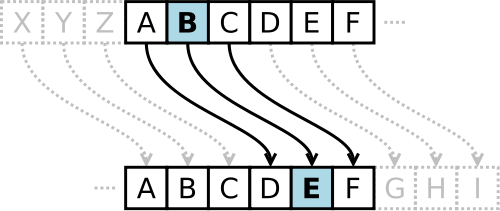
\includegraphics[scale=0.6]{./ConocimientosPrevios/imagenes/cifradoCesar.png}
  \caption{Ejemplo Cifrado Cesar}
  \label{fig:cifradoCesar}
\end{figure} 

	\item \textbf{Cifrado Homofónico:} Es una evolución del siguiente, pero en vez de sustituir siempre por el mismo carácter lo que se hace es tener la posibilidad de poder realizar varios cambios posibles, por lo que un mismo mensaje podría generar varios textos cifrados, complicando así su desencriptación. En la figura \ref{fig:cifradoHomofonico} podemos ver una tabla sencilla de sustitución para realizar el cifrado. Por ejemplo si ciframos la palabra ``PLATON" nos daría de resultado ``882110772963", pero podríamos sustituir la P no solo por 88 si no por cualquier valor de la tabla dando lugar a que pudiéramos crear varios mensajes cifrados.
	
\begin{figure}[h]
  \centering
    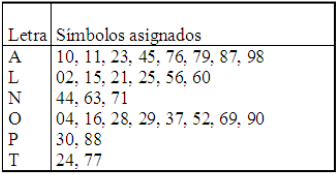
\includegraphics[scale=0.7]{./ConocimientosPrevios/imagenes/cifradoHomofonico.png}
  \caption{Tabla para cifrado homofónico}
  \label{fig:cifradoHomofonico}
\end{figure}

	\item \textbf{Cifrado por Transposición:} consiste en realizar una permutación de las posiciones que ocupan las letras escritas, un ejemplo podría ser escribir todo el texto con una cierta longitud preestablecida y luego leerlo por columnas en vez de por filas. En la figura \ref{fig:cifradoTransposicion} podemos ver un ejemplo del mecanismo de cifrado.  

\begin{figure}[h]
  \centering
    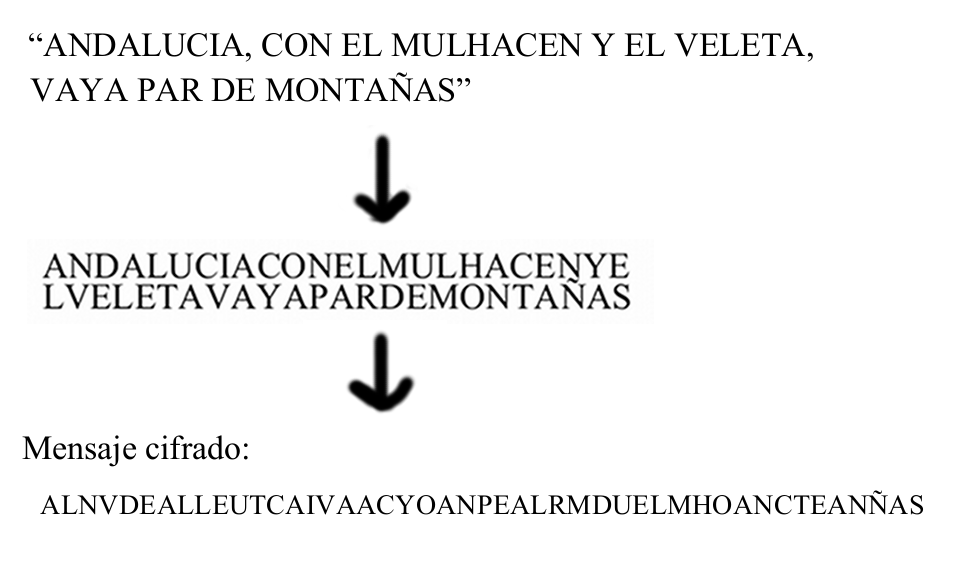
\includegraphics[scale=0.4]{./ConocimientosPrevios/imagenes/cifradoTransposicion.png}
  \caption{Ejemplo de cifrado por sustitución}
  \label{fig:cifradoTransposicion}
\end{figure}	

	\item \textbf{Cifrado Producto:} Es un cifrado que combina sustitución y transposición y se puede considerar como un encadenamiento de varios cifrados. Esto da lugar a cifrados complejos, seguros y difíciles de atacar, ya que tendríamos que averiguar no solo el método de cifrado utilizado, si no que también tendríamos que saber el orden en el que se ha ejecutado las encriptaciones.

	\item \textbf{Cifrado Vernam:} es un tipo de cifrado que se denomina cifrado de flujo. El texto en claro se combina con una cadena, del mismo tamaño del texto en claro, de número aleatorios o pseudoaleatorio por medio de la función XOR. Lo inventó Gilbert Vernam que era un ingeniero de AT\&T en 1917. Es también conocido como RC4 en internet.  
	
\end{itemize}

\subsection{Criptografía durante la época de los ordenadores.}

La criptografía dio un gran salto en cuanto a calidad en el momento en el que se pudieron empezar a usar ordenadores para encriptar y desencriptar textos, debido a que los ordenadores son máquinas que las tareas repetitivas las hacen muy bien y muy rápidos.

Se empezaron a idear nuevos algoritmos de cifrado mucho más complejos, los cuales se pueden dividir en dos grandes grupos, la criptografía de clave simétrica y la criptografía de clave pública.

A continuación vamos a explicar brevemente los algoritmos más famosos de estos dos grupos.

\subsubsection*{Criptografía de Clave simétrica}
	
Esta técnicas de criptografía se principal característica es que usan la misma clave para encriptar y desencriptar.
\begin{itemize}

	\item \textbf{Data Encryption Standard (DES):} Fue presentado por IBM en 1974, para generar un estandar para cifrado de transmisión de datos y para cifrado de almacenamiento de datos, para el gobierno, empresas privadas o cualquier tipo de usuario. IBM comenzó el desarrollo basándose en un dispositivo de cifrado llamado Lucifer el cual tenia una clave de 128 bits. Es un criptosistema de clave secreta que cifra en bloques de 64 bits del texto en claro y genera otros bloques de 64 bits del texto cifrado. La clave utilizada también es de 64 bits, pero el bit final de cada octeto de los 64 bits de la clave se usa como bit de paridad para control de errores. El cifrado se realiza en 16 iteraciones en las que se usan varias operaciones como son operaciones XOR, permutaciones y sustituciones. El esquema para cifrar se puede ver en la figura \ref{fig:cifradoDes}.
	
\begin{figure}
  \centering
    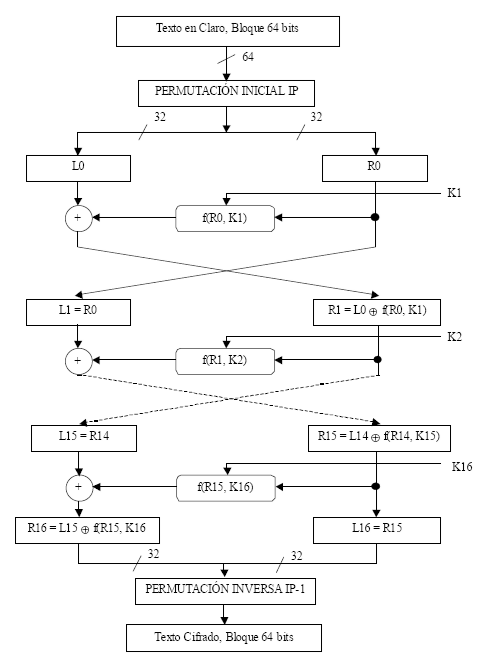
\includegraphics{./ConocimientosPrevios/imagenes/cifradoDes.png}
  \caption{Iteraciones en el cifrado DES}
  \label{fig:cifradoDes}
\end{figure}

\item \textbf{AES (Rijndael):} Fue presentado al concurso AES el 2 de enero de 1997 y anunciado ganador en 2001. Fue diseñado por dos criptólogos llamados Joan Daemen y Vincent Rijmen, ambos estudiantes de la Katholieke Universiteit Leuven de Bélgica. Al contrario que DES, AES es una red de sustituciones y permutaciones no una red de Feistel, se transformó en estándar efectivo el 26 de mayo de 2002 y en la actualidad es uno de los algoritmos de encriptación más famosos. Opera con bloques de 128 bits y tiene claves de 128, 192 y 256 bits.

\end{itemize}

El mayor problema que tiene este tipo de criptografía es que para que el destinatario pueda leer el mensaje necesita saber la clave y el intercambio de clave puede ser un problema muy grande, si los dos usuarios no se pueden comunicar directamente, ya que usando cualquier otro método podría ser interceptado y todo el proceso de encriptación no serviría de nada.

\subsubsection*{Criptografía de Clave Pública}

La criptografía de clave pública fue inventada por Diffie y Hellman y paralelamente por Merkle y ambos grupos aportaron a la criptografía el concepto de la utilización de pares de claves.

La característica principal es que cada usuario posee dos claves una privada que solo conoce el dueño de la clave y será usada para descifrar todo lo que otros usuarios cifren con su clave pública, así de esta forma si una persona quiere comunicarse con otra de forma secreta solo tiene que conocer su clave pública, cifrar con ella y el destinatario podrá desencriptar el mensaje con su clave privada. También posee una clave pública que será conocida por el resto de usuarios y que estos usarán para encriptar el mensaje que queremos que sea secreto. 

Otras características son que las claves son imposibles de deducir una a partir de la otra, cualquier usuario puede encriptar un mensaje con la clave pública pero no puede desencriptarla, ya que solo se puede desencriptar con la clave privada. Ambas claves son de una gran longitud y son generadas por exponenciación y/o productos de números primos grandes.

En los primeros años de existencia de la criptografía de clave pública se inventaron tres sistemas, Algoritmo de la mochila de Merkle-Hellman que fue roto, el esquema de McEliece que está considerado imposible de llevar a la práctica y un tercero que es el que explicaremos a continuación llamado RSA que es el más usado actualmente.

\begin{itemize}

	\item \textbf{RSA:} Su nombre proviene de sus creadores que son Rivest, Shamir y Adleman y se basaron en la idea de ``es muy fácil multiplicar dos números enteros primos grandes, pero extremadamente difícil hallar la factorización del producto" cuando inventaron el RSA en 1997. Se trata de un algoritmo exponencial. Tanto el mensaje como el texto cifrado tienen que ser un código decimal, por lo que se usaría por ejemplo el valor ASCII de la letra. Un ejemplo de uso sería el siguiente, lo primero que se debe de hacer antes de enviar el mensaje es acordar el algoritmo que se va a usar, lo siguiente el emisor cifra el mensaje usando la clave pública del receptor y lo envía por el método que el prefiera, acto seguido el receptor descifra el mensaje que ha enviado el receptor usando su propia clave privada, la gran ventaja de todo este método que soluciona el gran problema que dijismo que tenían los algoritmos de cifrado simétrico, que antes de nada había que intercambiar la clave con el problema que eso implicaba. 

\end{itemize}

%TODO: poner el número del capítulo
El algoritmo RSA será explicado con más profundidad en el capítulo de criptografía correspondiente.

Los algoritmos de clave pública tienen un gran problema y es que son muy lentos cifrando y descifrando por lo que en la vida real se suelen usar para intercambio de claves de algoritmos de clave simétrica que son mucho más rápido y también seguros.

\section{Android.}

Android es un sistema operativo basado en Linux especialmente diseñado para smartphone, tablet, smart TV y una infinidad de dispositivos, desarrollado por Google con Open Handset Alliance. Android empezó siendo desarrollado por la compañia llamada Android que inicialemente fue financiada y después comprada por Google en 2005. En 2007 cuando se presentó por primera vez Android también se anunción la fundación de Open Handset Alliance que es un conjunto de 86 empresas entre las que hay compañías de hardware, software y de telecomunicaciones, interesadas en el mundo de los dispositivos móviles. Android es código abierto y está distribuido bajo licencia Apache\footnote{Para saber más sobre la licencia visite: \url{http://en.wikipedia.org/wiki/Apache\_License}}. La tarea del mantenimiento y desarrollo de Android es de Android Open Source Project (AOSP).

Android tiene una gran comunidad de desarrolladores que pueden extender las funcionabilidades de los telefonos o dispositivos donde se pueda ejecutar android, android se puede desarrollar en Java usando el SDK de Android o en C++ usando el NDK de Android. Android posee una tienda online llamada Google Play (anteriormente Android Market) desde la que cualquier desarrollador por una pequeña cantidad de dinero (Alrededor de 25€ por una cuenta vitalicia de desarrollador) puede subir todas las aplicaciones que desee, de forma gratuita o pagada. En Junio de 2012 había alrededor de 600.000 aplicaciones en Google Play.

En el primer cuarto de 2012, Android tenia el 59\% del mercado de smartphones en el mundo, de ahí la importancia de esta plataforma para los desarrolladores, ya que proporciona un mercado muy amplio y una forma muy fácil y barata de conseguir un gran número de usuarios.

%TODO: poner capítulo.
Los detalles técnicos de android se explicarán con más profundidad en el tema de android

\subsection{Historia.}

Como hemos dicho anteriormente Android fue diseñado y creado originalmente por una compañía llamada Android que fue fundada en Palo Alto, California en 2003 por Andy Rubin, Rich Miner, Nick Sears y Chris White. Originalmente solo estaba diseñado para funcionar con smartphones ya que ellos pensaban que un smartphone era algo más que un dispositivo que sirviera para usar el GPS y tener preferencias. 

Google compró Android el 17 de agosto de 2005 con la intención de entrar en el mercado de los teléfonos móviles. Después de varios años de rumores el 5 de noviembre de 2007, Google presentó la Open Handset Alliance un grupo de empresas que incluian a Broadcom Corporation, Google, HTC, Intel, LG, Marvell Technology Group, Motorola, Nvidia, Qualcomm, Samsung Electronics, Sprint Nextel, T-Mobile and Texas Instruments entre otras muchas empresas que estaban interesadas en generar estándares para dispositivos móviles. Ese mismo día también se lanzó el primer producto android basado en el kernell de Linux 2.6.

Android ha sido muy criticado por la gran fragmentación que tiene debido al gran número de versiones que tiene, que son compatibles hacia abajo pero no hacia arriba, por lo que necesita que los fabricantes actualicen el software de sus teléfono lo que es un gran problema debido a que muchos no lo hacen, hubo un pequeño intento de solucionar este problema haciendo que los fabricantes sacaran actualizaciones en al menos en los 18 meses posteriores a la salida al mercado del terminal, pero al final no hubo ningún acuerdo.   

\subsection{Versiones.}

Como curiosidad todas las versiones de Android se denominan con un nombre en clave que es un postre.
\begin{itemize}

	\item \textbf{1.0 (Apple Pie):} primera versión lanzada el 23 de septibmre del 2008.
	
	\item \textbf{1.1 (Banana Bread):} lanzada el 9 de febrero del 2009.
	
	\item \textbf{1.5 (Cupcake):} fue presentada el 30 de abril del 2009, esta fue la primera versión con la que android empezó a despuntar y entrar en el mundo de los teléfonos móviles, anteriormente apenas si era conocido. Tenía características nuevas muy interesantes como poder grabar y reproducir video, podía subir videos a Youtube e imágenes a Picasa directamente desde el teléfono, un nuevo teclado predictivo, nuevos widget y carpetas para colocar en la pantalla de inicio y transiciones animadas.

	\item \textbf{1.6 (Donut):} fue presentada el 15 de septiembre de 2009. Se le añadieron las siguientes características nuevas como una interfaz ingrada para la cámara, la grabadora de video y la galería, se actualizó la búsqueda por voz añadiendo soporte a más aplicaciones nativas y la posibilidad de llamar a contactos, se añadió un buscador general en la pantalla de inicio donde se podía buscar contactos, historiales y páginas web, se añadió un nuevo framework de gestos y las herramientas de desarrollo llamado GestureBuilder.

	\item \textbf{2.0 / 2.1 (Eclair):} la versión 2.0 fue presentada el 26 de octubre de 2009 y la 2.1 fue liberada el 3 de diciembre del 2009. Se añadieron un gran número de mejoras, se optimizó la velocidad de hardware, se soportaron más tamaño de pantallas y resoluciones, se rediseñó la interfaz de usuario, el navegador también fue renovado y se le añadió soporte para HTML5, nueva lista de contactos, se añadió soporte para el flash de la cámara, zoom digital, soporte para bluetooth 2.1, se mejoraron la captura de eventos multi-touch con MotionEvent y fondos de pantalla animados.
	
	\item \textbf{2.2 (Froyo):} fue lanzada el 20 de mayo de 2010. Se optimizó el sistema Android, la memoria y el rendimiento, se mejoró la velocidad de las aplicaciones gracias a la implementación de JIT, se implementó el motor JavaScript V8 de Google Chrome en el navegador del móvil, nueva funcionalidad de WiFi hotspot y tethering por USB, se actualizó el android market para que tuviera actualizaciones automáticas, marcación por voz y compartir contactos por Bluetooth, soporte para contraseñas numéricas y alphanuméricas, soporte para Adobe Flash 10 y soporte para pantallas de Hdpi, como pueden ser pantallas de 4" y resolución de 720p. 

	\item \textbf{2.3 (Gingerbread):} fue presentado el 6 de diciembre del 2010. Cambiaron el diseño de la interfaz de usuario, añadieron soporte para pantallas extra grandes y resoluciones WXGA, soporte nativo para VoIP SIP, reproducción nativa de videos WebM/VP8 un formato de video patrocinado por Google que es la alternativa al H264 en la reproducción de video en HTML5 y decodificación de audios en AAC, se añadió soporte a NFC (Near Field Communication), nuevo teclado multitactic, soporte mejorado para programar en código nativo, soporte nativo de más sensores como pueden ser acelerómetros o barómetros, soporte para múltiples cámaras y cambio del sistema de archivos YAFFS a ext4. La versión 2.3.3 sigue siendo la versión de Android más usada actualmente. 

	\item \textbf{3.0 / 3.1 / 3.2 (Honeycomb):} Esta versión fue diseñada exclusivamente para tablet, por lo que no hubo smartphones que actualizaran a esta versión. Las características principales fueron un escritorio en 3D con widget rediseñado, sistema multitarea mejorado, mejoras en el navegador de internet, videochat mediante Google Talk, mejoras en el soporte de redes WiFi, añadidos soporte para gran cantidad de periféricos y conexión USB.
	
	\item \textbf{4.0 (Ice Cream Sandwich):} Fue una de las actualizaciones más importantes que ha recibido Android y fue lanzada el 19 de octubre de 2011, en ella se unificaron todas las versiones y se tenía una sola versión para smartphne, televisores, tablets, netbooks, etc. Se añadió una nueva versión de interfaz mucho más limpia y usable llamada Holo, una nueva fuente llamada Roboto, se da la opción de utilizar botones virtuales en la interfaz de usuario en vez de botones físicos, soporte para aceleración gráfica por hardware, por lo que la interfaz es manejada y dibujada por la GPU, aumentando notablemente el rendimiento, multitarea mejorada, se ha añadido un nuevo corrector ortográfico, en la lista de notificaciones se pueden eliminar las que no sean interesantes, capturas de pantalla pulsando el botón de encendido y el de bajar volumen, mejorada la aplicación encargada de hacer fotografías, añadida una nueva opción para crear fotos panorámicas, Android Beam, una nueva característica que nos permite compartir contenidos entre teléfonos mediante NFC, reconocimiento de voz del usuario, reconocimiento facial, para bloqueo y desbloqueo del teléfono, añadidas nuevas carpetas que se crean solo con arrastrar y soltar, un único y nuevo framework para crear aplicaciones y soporte para contenedor MKV.

	\item \textbf{4.1 (Jelly Bean):} Esta es la última versión de Android que hay en el mercado, fue lanzada el 27 de junio de 2012 durantes la última Google I/O. Se mejoró la fluidez y la estabilidad gracias al proyecto ``Project Butter", ajuste automático de widget cuando se añaden al escritorio, se añadió soporte para lenguas no occidentales, mejora de Android Beam para poder enviar video por NFC, dictado de voz mejorada y sin tener que tener conexión a internet para usarlo, nuevas notificaciones en las que se puede añadir botones para controlar o tener acceso a opciones más comunes, como puede ser responder a un email, pulsar pause o pasar de canción, nueva función Google Now que intenta ser el SIRI de Android, cifrado de aplicaciones y nuevas actualizaciones incrementales, en las que no es necesario volver a bajar toda la aplicación para actualizarla, solo se baja las partes nuevas, Google Chrome se convierte en el navegador por defecto de Android y se pone fin al soporte de Adoble Flash Player, se añade una nueva función llamada Sound Search que permite identificar la canción que está sonando, se ha añadido una nueva función llamada Gestual Mode para personas discapacitadas visualmente.
\end{itemize}

En el proyecto se ha usado la versión 4.0 para el desarrollo.

En la figura \ref{fig:android41} se puede como se ve visualemte android en la actualidad con la versión 4.1.

\begin{figure}
  \centering
    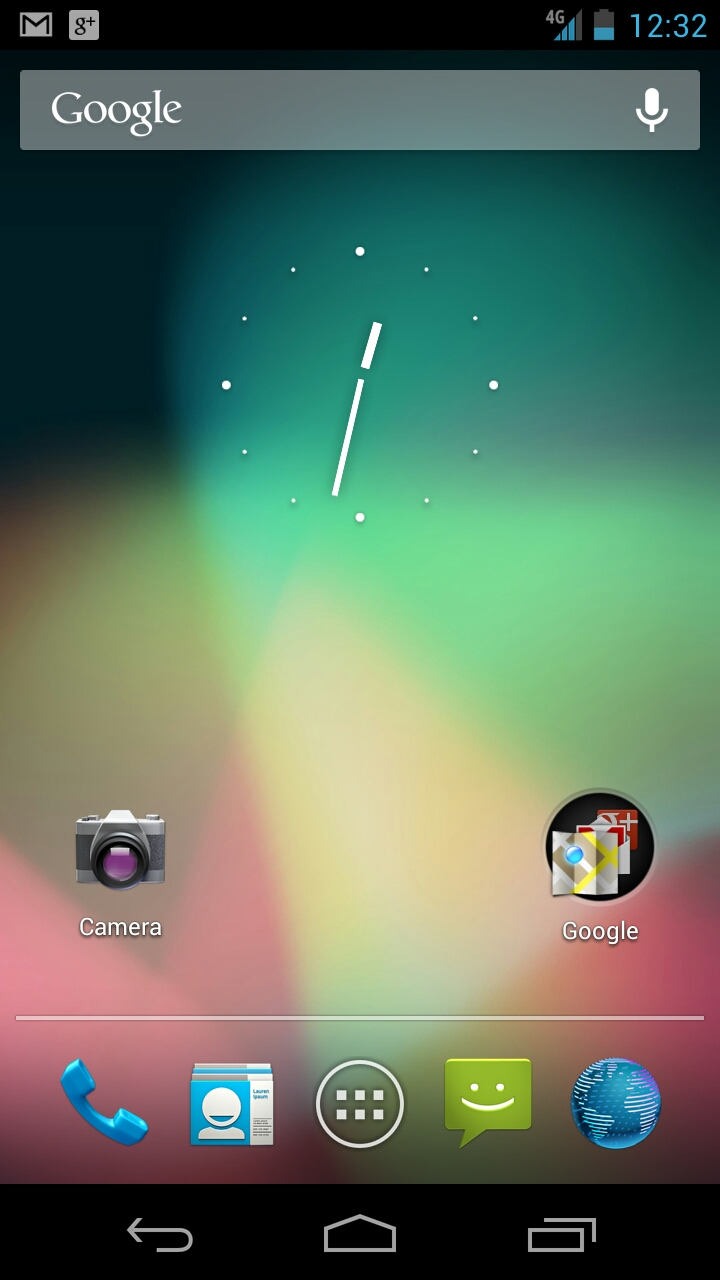
\includegraphics[scale=0.3]{./ConocimientosPrevios/imagenes/android41.jpeg}
  \caption{Versión de Android 4.1}
  \label{fig:android41}
\end{figure}


\section{Google App Engine.}

Google App Engine es un plataforma de cloud computing para desarrollar y almacenar aplicaciones web que ofrece Google. Las aplicaciones web pueden ser escalables y si necesitan más recursos automáticamente le son asignados para poder seguir ofreciendo servicio. Google App Engine es gratis para un cierto número de peticiones y almacenamiento, la primera versión fue lanzada en abril del 2008.

Actualmente se puede desarrollar en tres lenguajes, que son Java, Python y Go, este último un lenguaje propiedad de Google. En el proyecto hemos usado el lenguaje Java para desarrollar la aplicación web. 

Google App Engine para Java soporta muchos estándares y framework, y el Core está hecho con la tecnología servlet 2.5 usando el servidor de software libre llamado Jetty Web Server acompañado con otras tecnologías como JSP. El almacén de datos puede ser muy intuitivo pero se puede acceder facilmente con JPA y los métodos JDO para escritura y lectura de datos. También se pueden usar tecnologías como Spring Framework.

Google garantiza que aplicación estará disponible el 99.95\% del tiempo, al estar altamente replicada.

La base de datos a la que dan acceso no es una base de datos que tiene una sintaxis muy parecida a SQL pero es GQL, una de las principales características es que no admite sentencias join, debido a la ineficiencia de la misma. La versión de Java soporta consultas asincronas no bloqueantes, ofreciendo así una forma de procesamiento paralelo de datos.

Para más información se puede visitar la web diseñada para desarrolladores que proporciona Google, \url{https://developers.google.com/appengine/}. 

En el capítulo \ref{cap:GAE} veremos más ampliamente todo lo relacionado con Google App Engine que se ha usado en el proyecto.

\section{SQLite.}

SQLite es un sistema de gestión de bases de datos relacionadas compatibles con ACID, ACID es un acrónimo de Atomicity, Consistency, Isolation and Durability que son todas las características que deben de tener una bases de datos para que se consideren bases de datos relacional. La característica principal es que ocupa muy poco espacio alrededor de 275 Kb y fue escrita en C por Richard Hipp. Está distribuida bajo licencia de dominio público.

A diferencia de los sitemas de gestión de bases de datos clientes-servidor el motor de SQLite pasa a ser parte del programa que quiere usarlo ya que se integra con él. Esto hace que tenga mayor rendimiento debido a la comunicación por medio de funciones es mucho más eficiente que mediante comunicación de procesos. La totalidad de la base de datos, tablas, indices y los datos, se guardan en un solo fichero estándar en la máquina host. La versión 3 de SQLite permite base de datos de hasta 2 Terabytes y permite campos del tipo BLOB.

SQLite está muy extendido y se puede programar en infinidad de lenguajes de programación como pueden ser C, C++, Perl, Python, PHP, Java, etc.

Es utilizado en infinidad de programas y sistemas, que van desde editores de imagen como puede ser Adobe Photoshop Elements, reproductores de sonido como Clementine o navegadores como Firefox, Chrome u Opera.

Esta es una de las tres formas que proporciona Android para guardar datos, al estar embebida en cada aplicación para mejorar el rendimiento, cada aplicación debe de tener una. 

\section{XML.}

XML son las siglas en inglés de e\textbf{X}tensible \textbf{M}arkup \textbf{L}anguage que es un lenguaje de marcas desarrollado por el World Wide Web Consortium (W3C), deriva del lenguaje SGML y permite definir la gramática de lenguajes específicos para estructurar documentos grandes.

Es una de las formas de intercambio estructurado de información mas extendidas en internet, ya que se puede usar en base de datos, hojas de cálculo o en casi cualquier información que se quiera usar.

XML es un lenguaje que puede ser analizado sintáxticamente para averigurar si está bien formado o no, por lo que para que cualquier parser ( analizador sintáxtico ) confirme que es correcto debe te mantener una estructura que viene definida en el estándar. Todos los documentos tiene que tener las siguientes partes para que sean bien formados, prólogo, cuerpo, elementos y atributos.

Un ejemplo de la figura \ref{cod:XML} podemos ver un trozo de código XML para almacenar un libro en una librería.

\begin{figure}
\begin{small}
 \begin{center}

    
  \begin{lstlisting}[language=XML]   
<?xml version="1.0"?>
<libro>
<titulo> Cien años de soledad </titulo>
<disponible tiempo="24" unidad="horas"/>
<autor> Gabriel García Márquez </autor>
<formato> Rústica </formato>
<publicacion>1967 </publicacion>
<precio cantidad="9.99" moneda="euro"/>
<descuento cantidad="5"/>
<enlacelibro href="/exec/ISBN/84-473-0619-4"/>
</libro>
    
  \end{lstlisting}

\end{center}
\end{small}
  
  \caption{Código ejemplo XML.}
  \label{cod:XML}
\end{figure}

En el proyecto hemos usado XML para los archivos de configuración de android o para el diseño de las interfaces en android. En una de la aplicaciones web realizadas para los archivos de configuración también hemos usado XML, en la otra hemos usado un lenguaje parecido llamado YALM, que es equivalente a XML.

\section{UML.}

UML es un lenguaje de modelado de proposito general más usado en la actualidad para el diseño de software. UML son las siglas de Unified Modeling Language. UML tiene la ventaja de que se puede observar visualmente el diseño del software. Se puede desde especificar, construir o documentar un sistema o un software.

%Poner una imagen de ejemplo

%Mirar esto... xDDDD
Hemos usado UML para diseñar las clases usadas a lo largo de todo el proyecto, además de para mostrar en la memoria del proyecto la relación de las clases, los casos de uso...

\section{GIT.}

Git es un software de control de versiones a la vez que mantenedor al coherencia y cohesión del código fuente orientado a la velocidad. Fue desarrollado para el manejo del código fuente de linux y al principio fue diseñado por Linus Torvalds. GIT es un repositorio con un completo historial y una capacidad de identificación de cada cambio realizado sin depender del acceso a la red o a un servidor central. Está liberado con licencia GNU versión 2.

En el proyecto hemos estado usando GIT como control de versiones por si en algún cambio ocurría algún problema y debíamos volver atrás y para tener una copia de seguridad del proyecto alojado en todo momento en un servidor externo por si había algún fallo.

A lo largo del proyecto hemos usado dos servicios gratuitos como el conocido \url{https://github.com/} y \url{https://bitbucket.org/}. El primero es muy famoso actualmente y hay mucho software libre en dicha plataforma, tiene un probema y es que el código tiene que ser libre y en la versión gratuita no se pueden tener repositorios privados, cosa que en el segundo servicio si te los ofrece. Para todo el código fuente usando, tanto en la aplicación de android como en las dos aplicaciones hemos usado bitbucket y para la memoria de proyecto hemos usado github. La dirección del repositorio de la memoria es la siguiente: \url{https://github.com/t321/memoriaPFC}, el repositorio de las aplicaciones web \url{https://bitbucket.org/t321/pfcaeg} y el de la aplicación de Android \url{https://bitbucket.org/t321/pfcandroid}.

%TODO: poner el apendice
La configuración básica para el uso de GIT tanto con Eclipse como con la terminal se puede ver en el apendice !!!?????¿¿  















	%criptografía usada en el proyecto
	\chapter{Criptografía usada en el proyecto.}\label{cap:criptografia}

En la sección \ref{lbl:criptografia} del capítulo \ref{cap:conocimientos} hemos hecho una breve introducción a la criptografía de clave pública, a continuación vamos a explicarla con más extensión y los usos que le hemos dado en el proyecto.

Toda la criptografía que hemos usado es criptografía de clave pública, y en concreto el criptosistema llamado RSA. En el proyecto se ha usado la criptografía para firmar digitalmente, no para cifrar los mensajes.

\section{RSA.}

RSA se basa en la idea de que multiplicar dos números enteros primos, pero muy difícil sabiendo el resultado de la multiplicación averiguar dichos dos números.

El proceso de generación de las claves se va a explicar a continuación:
\begin{itemize}

	\item Se eligen dos números primos grandes que llamaremos \textbf{p} y \textbf{q}, dichos números se multiplican y obtenemos \textbf{n}, $n = p \cdot q$, dicho valor de $n$ es el que se usa como módulo de la clave pública y privada. 

	\item Calculamos $\varphi(n)$ de la siguiente forma $\varphi(n)=(p-1)\cdot(q-1)$, donde $\varphi(n)$ es la función $\varphi$ de Euler.

	\item Se elige un entero positivo $e$ menor que $\varphi(n)$ y que sea coprimo con $\varphi(n)$. El valor $e$ es el exponente de la clave pública.
	
	\item Se busca un valor $d$ que satisfaga la congruencia $d=e^{-1}\,mod\,\varphi(n)$. Este valor se suele calcular con el algoritmo de Euclides extendido y el valor $d$ es el exponente para la clave privada. 
\end{itemize}

La clave pública será $(n,e)$ y la clave privada será $(n,d)$.

El proceso de cifrado y descifrado es el siguiente:

\begin{itemize}
	\item \textbf{Cifrado:} el receptor (Alice) envía su clave pública $(n,e)$ al emisor (Bob) y guarda la clave privada, $(n,d)$, en secreto, a partir de este momento Alice usando la clave pública de Bob puede comunicarse seguramente. El mensaje que Bob quiere enviar a Alice será $M$. Bob primero convierte $M$ en un número menor que $n$, y que sea de una forma reversible de forma que sabiendo $n$ podamos volver a conseguir $M$. Acto seguido calcula $c$ de esta forma, $c\equiv m^e\,(mod\,n)$. Bob mandaría $c$ a Alice y la comunicación finalizaría.
	
	\item \textbf{Descifrado:} Alice empezará el proceso para recuperar $m$ a partir de $c$ y $d$. $m\equiv c^d\,(mod\,n)$, una vez ha calculado $m$ puede conseguir $M$.

\end{itemize}

El proceso de descifrado funciona porque $c^d=(m^e)^d\equiv m^{ed}\, (mod\, n)$ y hemos elegido $d$ y $e$ de forma que $e\cdot d =1+k\cdot\varphi(n)$, se cumple que $ m^{ed}\cdot m^{1+k\cdot\varphi(n)} = m(m^{\varphi(n)})^k = m\, (mod\, n)$, esta última congruencia se obtiene directamente del teorema de Euler cuando $m$ y $n$ son coprimos.

Un ejemplo de cifrado y descifrado mediante el algoritmo RSA es el siguiente:

\begin{itemize}

\item Elegimos $p=61$, $q=53$. Podemos observar que ambos son primos. Se ha elegido para el ejemplo unos valores pequeños para que podamos hacer los cálculos con facilidad.

\item Calculamos $n=p\cdot q= 3233$.

\item Elegimos $e=17$ y $d=2753$, como exponente público $e$ y como exponente privado $d$. La clave pública quedaría como $(17, 3233)$ y la clave privada sería $(2753, 3233)$.

\item La función de cifrado quedaría como la siguiente: $\mbox{encrypt}(m) = m^e \,mod(n) = m^{17}\,mod(3233)$, donde $m$ es el texto sin cifrar. Imaginemos que $m=123$, luego los cálculos quedarían, $\mbox{encrypt(123)} = 123^{17}\,mod(3233) = 855$.

\item La función de descifrado sería: $\mbox{decrypt(c)} = c^d\,mod(n) = c^{2753}\,mod(3233)$, donde $c$ es el mensaje cifrado. Usando la función para descifrar $c=855$ obtenemos lo siguiente: $\mbox{decrypt(855)} = 855^{2753}\,mod(3233) = 123$.

\end{itemize}

Podemos observar que hemos conseguido cifrar y descifrar de forma segura usando dos claves diferentes y una de ellas es pública.

Una de las característica del algoritmo RSA es que permite la verificación de la veracidad de documentos mediante un proceso que se llama firma digital. Con ello no garantizamos que un atacante no pueda leer el mensaje, ya que no nos importa, pero si podemos garantizar que dicho mensaje no ha sido modificado. 

La forma de realizar la firma es la siguiente, en vez de firmar todo el documento, que sería un gran problema ya que estos algoritmos son muy lentos, Alice genera un hash del documento con una longitud fija (128 o 256 bits) y se firma dicho hash con su firma privada. Una función hash es una función matemática que para una entrada devuelve un valor único, por lo que podemos garantizar que un documento sólo va a devolver un valor numérico único y si modificamos algo del documento ese valor se alterará. Acto seguido se envía el valor de la función hash firmado junto con el documento original. Cuando Bob recibe el mensaje lo único que tiene que hacer es volver a generar el hash del documento de la misma forma que lo hizo Alice y usando la clave pública de Alice descifrar el hash firmado. Si ambos valores son iguales podemos garantizar que el mensaje es el original que Alice quería enviar.

En el proyecto hemos usado librerías que proporciona Java en su API \lstinline{java.security.*}. En dicha librería, como veremos en la sección \ref{cap:javasecurity} con más profundidad, se nos proporcionan todas las utilidades para manejo y creación de claves públicas y privadas, keystores, certificados de clave pública, funciones hash, algoritmos como RSA o DSA y algoritmos de cifrados simétricos, etc. 

Generalmente cuando se intercambian las claves no se pasan los números en un par como hemos hecho anteriormente ya que los números primos no son de dos dígitos son números primos muy grandes, se usan contenedores de certificados de claves en los que van incluidos ambas claves o sólo la pública, además de más datos como entidades que verifican que el certificado es real. Uno de los grandes problemas que tiene la criptografía de clave pública es que cualquiera puede generar un certificado y decir que es otra persona, por lo que se necesita de entidades ajenas y que no tengan ningún compromiso con ninguna de las partes. Esto es lo que se llama una PKI (Public-Key Infrastructure).

\section{Public-Key Infrastructure.}

Una PKI es una combinación de hardware, software, políticas y procedimientos de seguridad que garantizan las operaciones de cifrado, firma digital y el no repudio de las transacciones electrónicas y que se encargan de crear, almacenar, distribuir, usar y revocar los certificados digitales usados por empresas y particulares para garantizar las comunicaciones electrónicas. Esto se puede garantizar gracias a autoridades de certificación, que son empresas o entidades públicas que garantizan todo lo anterior.

Hay varias entidades dentro del sistema como puede ser una CA (Certificate Authority) que es la entidad que firma todos los certificados, sólo se usa para auto firmarse el certificado de ella y para firmar a las entidades certificadoras subordinadas, si este nodo del sistema es comprometido, toda la estructura caerá. Las autoridades subordinadas son las encargadas de certificar digitalmente a un usuario y garantizar que el usuario es real y de verdad es quien dice ser.  Las VA (Validation Authority) es la autoridad que se encarga de comprobar el estado del certificado emitido, si es válido o está revocado. Para asegurar que cada clave pública es única y pertenece a un usuario real se usa una RA (Registration Authority), la cual se encarga de verificarlo. Hay otra entidad importante que son los repositorios para almacén de certificados y los repositorios de listas de revocación de certificados. La lista de revocación es un componente muy importante de la PKI, ya que en dicha lista están los certificados revocados antes del tiempo indicado dentro del certificado. También suelen incluir TSA (TimeStamp Authority) que es la encargada de certificar que la operación fue realizada en tiempo en concreto.

\begin{figure}
  \centering
    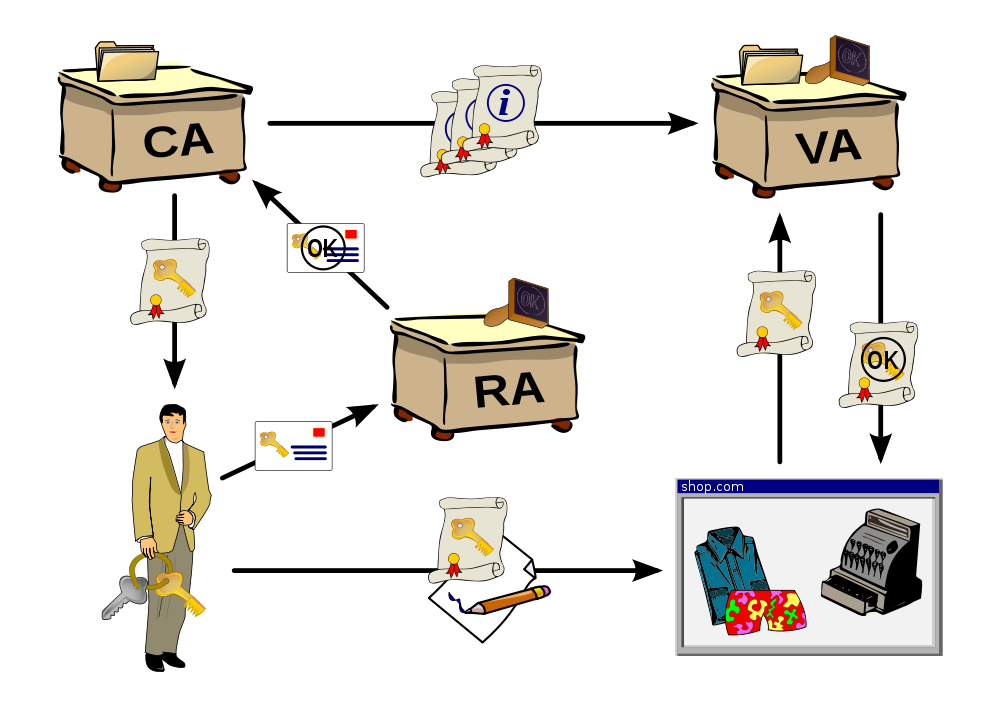
\includegraphics[scale=0.3]{./Criptografia/imagenes/esquemaPKI.png}
  \caption{Estructura genérica de una PKI.}
  \label{fig:esquemaPKI}
\end{figure} 

En la figura~\ref{fig:esquemaPKI} podemos ver todas las autoridades y sus relaciones que hemos explicado anteriormente.

En España tenemos dos PKI, una creada por la FNMT y otra creada por la Policía Nacional para dotar al DNIe de todos los certificados necesarios para que se pueda verificar la veracidad de un usuario de forma telemática. Tiene una estructura en la que hay una CA principal que está en la raíz y de ella cuelgan tres autoridades certificadoras subordinadas las emiten los certificados que se usan en el DNIe. La VA serían las comisarías donde se consigue el DNIe, donde se tiene que certificar que eres esa persona para conseguir el DNIe. En la figura \ref{fig:pkiDnie} se puede ver la estructura.

\begin{figure}
  \centering
    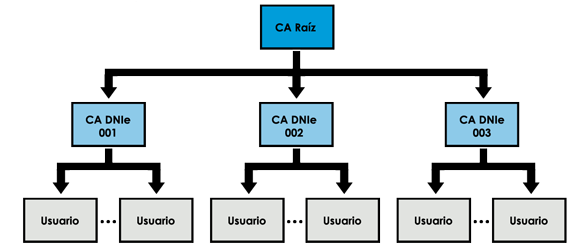
\includegraphics[scale=0.9]{./Criptografia/imagenes/pkiDnie.png}
  \caption{Jerarquía de la PKI del DNIe.}
  \label{fig:pkiDnie}
\end{figure} 

Una PKI puede garantizar la veracidad de la autentificación frente a otros usuarios y proporciona métodos para conseguir certificados de identidad de otros usuarios para firmar digitalmente, cifrar y descifrar. En toda operación hay tres pasos principales, el primero es el inicio de un usuario de la operación, el segundo un sistema de servidores que dan fe de que la operación ha ocurrido y garantizan la veracidad, como puede ser servidores de timestamp, la autoridad de certificación y la autoridad de registro, el tercer paso es el receptor recibe los datos firmados o cifrados y puede garantizar la veracidad de los documentos.

La tecnología PKI se puede usar para los siguientes casos, autentificación de usuarios y sistemas, identificación del interlocutor, cifrado de datos digitales, firmado digital de datos, tales como documentos, software, etc, asegurar comunicaciones y garantía de no repudio.

Existen varios tipos de certificados entre los que podemos encontrar certificados de tipo personal, que acredita la identidad del titular, un certificado de pertenencia a una empresa, que además de garantizar la identidad garantiza la empresa para la que trabaja, certificado de representante, que acredita los poderes que tiene dicho usuario sobre la empresa, certificado de servidor seguro, que utilizan los servidores para asegurar las conexiones con sus clientes, certificados de firma de código para garantizar que los cambios realizados en el código son legítimos y muchos otros tipos.

En el ámbito de servidores y sistemas informáticos hay varias PKI importantes como Verisign\footnote{ Se puede ver toda la información en su página web: \url{http://www.verisign.com/}} o Comodo\footnote{ Se puede ver toda la información en su página web: \url{http://www.comodo.com}}.  


En el proyecto hemos usado certificados generados por una CA imaginaria, en el anexo~\ref{cap:anexoB} podemos ver como generar certificados para poder hacer las pruebas, pero si el proyecto se realizara podría ser fácilmente extensible con una PKI propia de la Universidad de Málaga o con cualquiera que dote a todo el sistema de validez legal en España.

\section{Criptografía en Java.}\label{cap:javasecurity}

Como ya hemos dicho Java dota de una API llamada \lstinline{java.security}, donde proporciona todo tipo de algoritmos para la realización de funciones hash, firmas digitales, cifrados, generación de números aleatorios, etc. En \url{http://docs.oracle.com/javase/6/docs/technotes/guides/security/} podemos encontrar la documentación necesaria sobre todos los métodos de cifrado o firmado que proporciona la API.

El paquete \lstinline{java.security.*} proporciona diferentes clases que vamos a explicar a continuación:



\textbf{MessageDigest:} es la clase que proporciona todos los mecanismos para realizar funciones hash. La generación de un hash se puede observar en la figura~\ref{fig:messageDigest}. 

\begin{figure}[h]
  \centering
    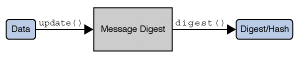
\includegraphics[scale=1.3]{./Criptografia/imagenes/messageDigest.png}
  \caption{Uso de la clase MessageDigest.}
  \label{fig:messageDigest}
\end{figure} 

La forma de uso es la siguiente, primero se genera un objeto del tipo \lstinline{MessageDigest}, el objeto se inicializa con la función \lstinline{getInstance()} de la fábrica de métodos estáticos que proporciona la clase, acto seguido se usa el método \lstinline{update()} para añadir los byte del mensaje al que queremos realizar la función hash y seguidamente usamos la función \lstinline{digest()} que devuelve el hash del mensaje que hemos introducido con el método \lstinline{update()}. Un ejemplo de esto se puede ver en el código que se muestra a continuación.

\begin{lstlisting}[style=Java] 
MessageDigest md = MessageDigest.getInstance("SHA");
md.update(toChapter1);
byte[] toChapter1Digest = tc1.digest();
\end{lstlisting}

\textbf{Signature:} es la clase que proporciona todos los métodos de firmado mediante algoritmos RSA o DSA. En la figura \ref{fig:signature} podemos ver el modo de uso. Para usarlo primero hay que poseer una clave (Key), puede ser una clave pública o privada y dependiendo de cual poseamos podemos firmar o verificar una firma. En el proyecto hemos usado la instancia \lstinline{SHA1withRSA}.

\begin{figure}[h]
  \centering
    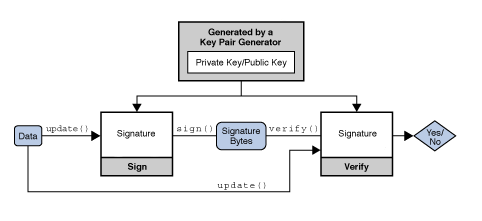
\includegraphics[scale=0.8]{./Criptografia/imagenes/signature.png}
  \caption{Modo de uso de la clase Signature.}
  \label{fig:signature}
\end{figure} 

El uso es muy parecido a la clase de \lstinline{MessageDigest}, lo primero es crear un objeto usando la función \lstinline{getInstance()} de la fábrica de clases con la instancia que queramos usar, acto seguido usamos el método \lstinline{initSign(Key)} con la que añadimos la clave al proceso, a continuación usamos el método \lstinline{update()} y añadimos los datos que queremos firmar o verificar. Si lo que queremos es firmar usamos la función \lstinline{sign()} y si queremos verificar usaremos la función \lstinline{verify()}. La función \lstinline{sign()} devuelve un array de bytes que sería la firma de los datos y la función \lstinline{verify()} devuelve un booleano con valor \lstinline{true} si la firma es válida o \lstinline{false} si no se puede verificar.

En el siguiente trozo de código podemos observar como se firma un mensaje. 

\begin{lstlisting}[style=Java] 
Signature instance = Signature.getInstance("SHA1withRSA");
instance.initSign(key);
instance.update((plainText).getBytes());
byte[] signature = instance.sign();
\end{lstlisting}

En este otro trozo de código podemos ver como se verifica un mensaje. 

\begin{lstlisting}[style=Java] 
Signature instance = Signature.getInstance("SHA1withRSA");
instance.initSign(key);
instance.update((cipherText).getBytes());
boolean verify = instance.verify();
\end{lstlisting}

\textbf{Cipher:} es una de las clases que más posibilidades ofrece, ya que implementa un gran número de algoritmos de cifrado simétrico. En la figura \ref{fig:cipher} se puede observar la forma de uso. 

\begin{figure}[h]
  \centering
    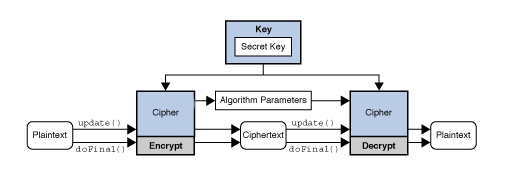
\includegraphics[scale=0.8]{./Criptografia/imagenes/cipher.png}
  \caption{Modo de uso de la clase Cipher.}
  \label{fig:cipher}
\end{figure} 

En el proyecto no hemos usado criptografía de clave simétrica, pero lo explicaremos de todas formas, ya que la forma de uso es sencilla. Se genera un objeto usando la fábrica de objetos que proporciona la clase con \lstinline{getInstance()} pasandole como parámetro una cadena con el algoritmo que queremos usar, como puede ser DES, AES, etc, junto con el padding, si es necesario, que vamos a utilizar. Un ejemplo es \lstinline{DES/CFB8/NoPadding} o \lstinline{DES/OFB32/PKCS5Padding}, acto seguido debemos de usar el procedimiento \lstinline{init()} donde debemos de indicar si el objeto se va a usar para encriptar o desencriptar y la clave usada, para finalizar podemos usar la función \lstinline{doFinal()} a la que le pasaríamos el texto cifrado o el texto en claro dependiendo del proceso que queramos usar.

Existen varias clases que se basan en la clase Cipher para cifrado de flujos o archivos enteros sin tener que ir byte a byte. Por ejemplo \lstinline{CipherInputStream} y \lstinline{CipherOutputStream}. 

\textbf{Key:} para el manejo de las claves dentro del paquete hay una interfaz con la que se manejan todo tipos de claves, desde claves públicas y privadas hasta claves de cifrado simétrico. Esta interfaz la implementan un gran número de clases como pueden ser \lstinline{PrivateKey}, \lstinline{PublicKey}, \lstinline{SecretKey}, \lstinline{RSAPrivateKey}, \lstinline{RSAPublicKey}, \lstinline{DSAPrivateKey}, \lstinline{DSAPublicKey}, etc. Para generar las claves hay que usar clases factoría como pueden ser \lstinline{KeyGenerator}, \lstinline{KeyPairGenerator} o \lstinline{KeyFactory} dependiendo de si queremos generar una clave simétrica o un par de claves o usar \lstinline{KeyStore} si lo que queremos es cargar llave de un llavero (archivo de claves) que tengamos.

En el proyecto no hemos tenido que generar claves, ya que queríamos que se pudiera cargar un llavero con la clave privada y pública, en el trozo de código siguiente podemos ver como se usa la clase \lstinline{KeyStore} en el proyecto.

\begin{lstlisting}[style=Java] 
KeyStore ks = KeyStore.getInstance("PKCS12");
ks.load(new FileInputStream(path), password.toCharArray());
PrivateKey key = (PrivateKey) ks.getKey(ks.aliases().nextElement(), password.toCharArray());
\end{lstlisting}

Como podemos ver lo primero que tenemos que hacer es generar un objeto \lstinline{KeyStore}, usando la función \lstinline{getInstance()} a la que le pasaremos como parámetro el tipo de llavero que vamos a usar, nosotros hemos usado PKCS12\footnote{Para más información visite \url{http://en.wikipedia.org/wiki/PKCS12}.}, que es un archivo creado especialmente para el almacenado de claves. Acto seguido cargamos el fichero, con el método \lstinline{load()}, al cual le pasaremos la ruta donde está el archivo físicamente y el password del archivo PKCS12. Para conseguir la clave privada usamos la función \lstinline{getKey()}, a la que hay que pasarle el alias con el que está guardada la clave en el llavero y el password. En el código se puede ver un casting, ya que la función \lstinline{getKey()} devuelve un elemento que implementa la interfaz \lstinline{Key}, pero nosotros sabemos que es un objeto de la clase \lstinline{PrivateKey}. De esta forma ya podemos usar la clave para firmar lo que necesitemos.


	%android
	\chapter{Android}\label{cap:android}


\section{Introducción.}

Android es un sistema operativo basado en Linux, libre y multiplataforma. Inicialmente empezó como un sistema operativo solo para móviles pero con el tiempo ya podemos encontrarlo en móviles, tablets, pc, neveras, relojes, cámaras de fotos y una gran cantidad de aparatos.

En el proyecto lo usaremos para diseñar y desarrollar una aplicación móvil, con la que poder firmar digitálmente un texto leido previamente mediante un lector de códigos QR.

Android es propiedad de Google actualmente y es el encargado de dar soporte y ayudar a los desarrolladores. Esta función la realiza muy bien, dando una muy buena API y una gran documentación. Podemos encontrar toda la información que podemos necesitar para desarrollar una aplicación en la siguiente web, \url{http://developer.android.com/index.html}. En la anterior web podemos encontrar la documentación de la API, consejos de diseño para que la aplicación tenga un aspecto bonito a la vez que usable, todas las novedades incluidas en las versiones nuevas del sistema operativo, etc.

\section{Arquitectura de la plataforma Android.}

Como hemos dicho anteriormente Android es una plataforma que engloba desde el sistema operativo, al software intermedio que comunica el sistema operativo y las aplicaciones, llamado en inglés middleware y las posibilidad de hacer funcionar las aplicaciones en la plataforma elegida, ya sea un telefono, una tables o cualquier aparato con Android.

Para los desarrolladores Android proporciona dos kit de desarrollo, uno que usa la tecnología Java (SDK), el que hemos usado durante el proyecto y otro que da la posibilidad de programar a más bajo nivel (NDK), este último desarrollado en C++.

El SDK de Android proporciona ayuda para las siguientes características, un navegador basado en WebKit, graficos optimizados en 2D, gráficos en 3D basados en OpenGL ES 1.0 con aceleración gráfica, una base de datos para almacenar datos que necesitemos, llamada SQLite, soporte para ficheros gráficos (JPG, PNG, GIF, etc), de vídeo (MPEG4, H.264) y audio (MP3, AAC), telefonía GSM, tecnologías inalámbricas como son Bluetooth, 3G, Wifi, uso de cámaras, GPS, brújulas, etc. Además de todo esto proporciona ayuda en la reutilización y remplazo de componentes, una máquina virtual optimizada para dispositivos móviles llamada Dalvik y un emulador donde poder probar antes del lanzamiento de la aplicación sin tener que poseer un móvil Android. 

\begin{figure}
  \centering
    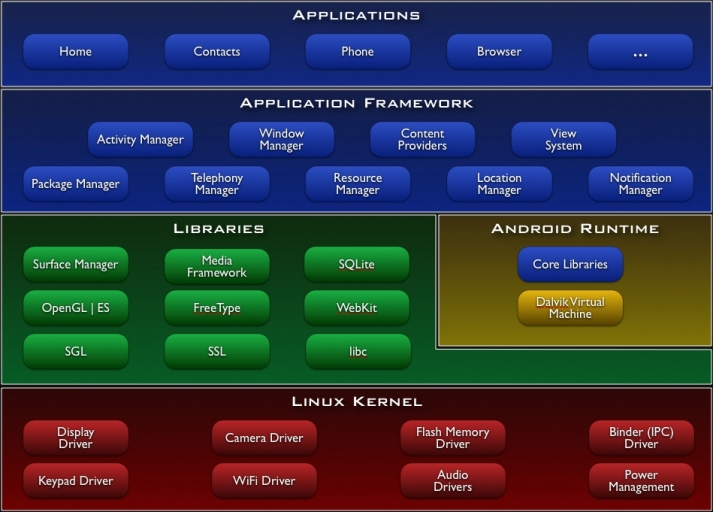
\includegraphics[scale=0.6]{./Android/imagenes/arquitecturaAndroid.jpg}
  \caption{Arquitectura de Android.}
  \label{fig:arquitecturaAndroid}
\end{figure} 

La arquitectura se puede ver en la figura \ref{fig:arquitecturaAndroid}. En ella se pueden ver las cinco capas principales en las que se divide Android.
\begin{itemize}

\item \textbf{Applications:} en esta capa están todas las aplicaciones que nos proporciona el sistema operativo de base, como pueden ser la lista de contactos, un gestor de SMS, el navegador, el lanzador de aplicaciones, todas las aplicaciones de servicios de Google, como pueden ser Gmail, Google Maps, Google Calendar, Google Reader.   

\item \textbf{Application framework:} en esta capa está todo lo relacionado con los manejadores de activitys, llamadas de telefono, controladores de vistas. Es una capa que hay intermedia para manejo de hardware, con la que se pueden controlar tanto las notificaciones, como servicios que se ejucuten en segundo plano, etc. Los desarrolladores tienen el mismo acceso mediante esta capa de la API a todos los servicios que las aplicaciones nativas que proporciona el sistema el operativo. 

\item \textbf{Libraries:} como su nombre indica en esta capa están todas las librerías que el sistema operativo necesita, para manejo de archivos multimedia, manejo de gráficos 3D, renderizado web, etc.

\begin{itemize}
	\item \textbf{System C library:} una implementación del estandar C, optimizada para funcionar en sistemas móviles para las funciones del kernell de linux.
	\item \textbf{Media Libraries:} librerías basadas en PacketVideo's OpenCORE para grabación y reproducción de formatos de audio y video mas populares del momento como MP3, H.264, JPG o PNG.

	\item \textbf{Surface Manager:} librería para manejo de graficos 2D y 3D para varias aplicaciones.

	\item \textbf{LibWebCore:} motor de renderizado para navegadores embebidos de páginas web.

	\item \textbf{SGL:} motor para renderizado 2D.

	\item \textbf{3D libraries:} librería que implementa la API de OpenGL ES 1.0, que proporciona aceleración 3D por hardware si es posible o una alta optimización para renderizado por software en sistemas que no posean aceleración por hardware.

	\item \textbf{FreeType:} librería para manejo de fuentes, tanto bitmap como vectoriales.

	\item \textbf{SQLite:} librería para el manejo de la base de datos que proporciona Android.

\end{itemize}

%si hablo de la máquina virtual algo más poner una referencia.
\item \textbf{Android Runtime:} es una capa que está al mismo nivel que la capa de librerías. En esta capa se añaden muchas librerías para dotar de la mayoría de las funcionalidades que proporciona Java, también está en esta capa la máquina virtual (Dalvik) encargada de ejecutar el código Smali de los archivos DEX.

\item \textbf{Linux Kernel:} Android está basado en el kernel de Linux 2.6 y todo lo relatico a seguridad, manejo de memoria, control de procesos, pila de protocolos de red y modelo de drivers es el mismo. El kernel es el que proporciona una capa de abtracción entre el hardware y el software que usará Android.

\end{itemize}

Como ya hemos dicho antes Android corre con cada aplicación en una máquina virtual, esta máquina virtual recibe el nombre de Dalvik. Dicho nombre viene de un pueblo de Islandía donde viven los familiares del creador de esta, Dan Bornstein. La máquina virtual ejecuta un byte code especial llamdo DEX (Dalvik Executable), que está especialmente diseñado y optimizado para funcionar en sistemas móviles, tablets, etc. En la figura \ref{fig:maquinaVirtualDalvik} podemos ver todo el proceso desde la creación del archivo JAVA a la ejecución.

\begin{figure}
  \centering
    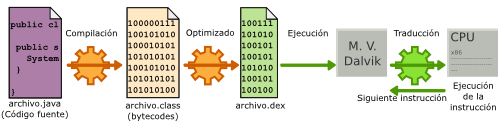
\includegraphics[scale=0.8]{./Android/imagenes/maquinaVirtualDalvik.png}
  \caption{Proceso de ejecución en Android.}
  \label{fig:maquinaVirtualDalvik}
\end{figure}


Los ficheros DEX meten las cadenas duplicadas y las constantes en un mismo fichero para ahorrar espacio, normalmente los archivos DEX suelen ser más pequeños que los archivos JAR de la máquina virtual de Java. Una vez instados los archivos DEX pueden ser modificados en el terminal para añadir optimizaciones, reordenado de byte en ciertos datos, quitado de clases vacias, etc. En la versión 2.2 de Android se añadió una nueva característica llamada JIT (just-in-time) que es compilación en tiempo real de los archivos DEX, por lo que se pueden añadir nuevas optimizaciones dependiendo de la plataforma.

Todas las aplicaciones de Android se distribuyen en unos archivos con extensión APK. Estos archivos no son más que archivos ZIP con la extensión cambiada. Todos deben de tener una estructura idéntica, que se explica a continuación. Contiene diferentes carpetas en las que se incluyen ficheros de configuración o necesarios para la aplicación y para comprobar la integridad de los archivos.

\begin{itemize}

\item \textbf{META-INF:} en un directorio que contiene tres archivos, \textit{MANIFEST.MF} que es el archivo de manifest, \textit{CERT.RSA} que es el certificado con el que está firmada la aplicación, \textit{CERT.SF} que contiene el hash en SHA-1 de todos los componentes de la aplicación, un ejemplo del archivo \textit{CERT.SF} es el siguiente:

\begin{verbatim}
Signature-Version: 1.0
Created-By: 1.0 (Android)
SHA1-Digest-Manifest: wxqnEAI0UA5nO5QJ8CGMwjkGGWE=
...
Name: res/layout/exchange_component_back_bottom.xml
SHA1-Digest: eACjMjESj7Zkf0cBFTZ0nqWrt7w=
...
Name: res/drawable-hdpi/icon.png
SHA1-Digest: DGEqylP8W0n0iV/ZzBx3MW0WGCA=
\end{verbatim}

\item \textbf{lib:} esta carpeta puede contener otras dependiendo de la plataforma para la que esté diseñada la aplicación. Si por ejemplo tiene código específicamente diseñado para x86 tendrá una carpeta llamada x86, si tiene código para MIPS una llamada mips donde estaría el código especialmente diseñado para esta plataforma. Puede que dicha carpeta no exista.

\item \textbf{res:} este directorio contiene los recursos que no tienen que ser compilados, como pueden ser las imágenes, los sonidos, etc.

\end{itemize}

Además de estas carpetas todos incluyen estos tres archivos.

\begin{itemize}
\item \textbf{AndroidManifest.xml:} es un archivo que sirve para indicar la versión, los permisos que contiene la aplicación, las referencias a librerías, las activitys que contiene la aplicación. En el siguiente listado podemos observar un extracto de los permisos que usamos en la aplicación del proyecto.

\begin{lstlisting}[style=XML]
 <uses-permission android:name="android.permission.INTERNET" />
<uses-permission android:name="android.permission.WRITE_EXTERNAL_STORAGE" />
<uses-permission android:name="android.permission.WRITE_SETTINGS" />
<uses-permission android:name="android.permission.GET_ACCOUNTS" />
<uses-permission android:name="android.permission.USE_CREDENTIALS" />
<uses-permission android:name="android.permission.MANAGE_ACCOUNTS" />
\end{lstlisting}

Podemos ver que con esto garantizamos que la aplicación pueda conectarse a internet, usar la tarjeta SD y manejar las cuentas almacenadas en el móvil, como puede ser la dirección de correo usada para dar de alta el móvil en Google Play.

\item \textbf{classes.dex:} el archivo DEX donde están todas las clases precompiladas en byte code para la máquina virtual Dalvik.

\item \textbf{resources.arsc:} es un fichero que contiene los recurdos precompiados como pueden ser los XML de las interfaces de la aplicación, etc.

\end{itemize}

\begin{figure}
  \centering
    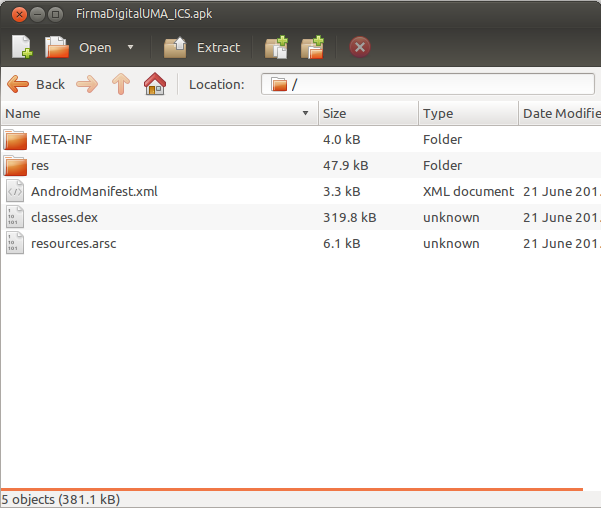
\includegraphics[scale=0.8]{./Android/imagenes/estructuraAPK.png}
  \caption{Estructura del fichero APK del proyecto.}
  \label{fig:estructuraAPK}
\end{figure}
 
En la imagen \ref{fig:estructuraAPK} se pueden observar los ficheros y las carpetas comentadas anteriormente del proyecto.

Toda aplicación en Android se contruye con unos componentes básicos como pueden ser activities, intents, views, services, contents providers, widgets y un largo etcétera. A continuación vamos a explicar los más importantes.

\begin{itemize}

%poner sección
\item \textbf{Activity:} una activity es la entidad más básica de una interfaz de usuario en la que se puede mostrar información en android, podemos pensar que es como una ventana de cualquier aplicación de escritorio. Cada interfaz que vemos en una aplicación de Android es un activity. Android tiene un ciclo de manejo de activitys bastante complejo, se explicará en la sección !!??!?!? donde pondremos más incapié en el desarrollo de la aplicación móvil del proyecto.

\item \textbf{Intent:} un intent es un componente practicamente imprescindible en cualquier aplicación de Android, es una forma de comunicación entre cualquier componente. Se pueden definir como mensajes o peticiones, ya que también puede comunicar aplicaciones entre sí. En el proyecto usamos intent para comunicar las activities y poder pasarnos datos, también la usamos para abrir el lector de códigos QR que necesitamos, dentro de nuestra aplicación llamamos al intent que nos proporciona la aplicación lectora y cuando termine ella nos devuelve el valor que había en el código QR para que podamos tratarlo.

\item \textbf{View:} son los componentes básicos con los que podemos contruir las interfaces gráficas, como pueden ser botones, barras de texto, campos de texto, spinner, etc. Android pone a nuestra disposición una gran cantidad de estos elementos, y además brinda la posibilidad de crear nuevos, según los vayamos necesitando. Estos objetos normalmente se añaden a una vista y se pueden añadir, modificar o borrar en ella. Estos objetos tienen un ID único en la aplicación por el que podemos controlarlo y añadirle por ejemplo el texto si es un campo de texto o un listener si es un botón para que cuando se pulse realizar la acción que necesitemos.

En el proyecto no hemos tenido que generar controles nuevos, nos hemos bastado con los que vienen por defecto.

\item \textbf{Services:} un servicio es un componente de Android que no tiene interfaz gráfica asociada y se ejecuta en segundo plano. Es similar a los servicios que ofrece cualquier sistema operativo. Pueden realizar cualquier acción, tanto recoger o actualizar datos, lanzar notificaciones cada cierto tiempo o mostrar activity para que el usuario introduzca algún valor que necesite.

\item \textbf{Content Provider:} es un mecanismo que posee android para intercambiar información entre aplicaciones. Por ejemplo cuando usamos la opción de compartir en el teléfono, dentro de una aplicación, nos salen varias aplicaciones con las que podemos compartir directamente, estas son todas las aplicaciones que han implementado el content provider que necesita esta aplicación para compartir la información. En la figura \ref{fig:contentProvider} podemos ver la opción de compartir de una aplicación y podemos observar como aparece por ejemplo GMail para mandar un email directamente desde aquí sin tener conocimiento de como se produce el intercambio de datos.
 
\begin{figure}
  \centering
    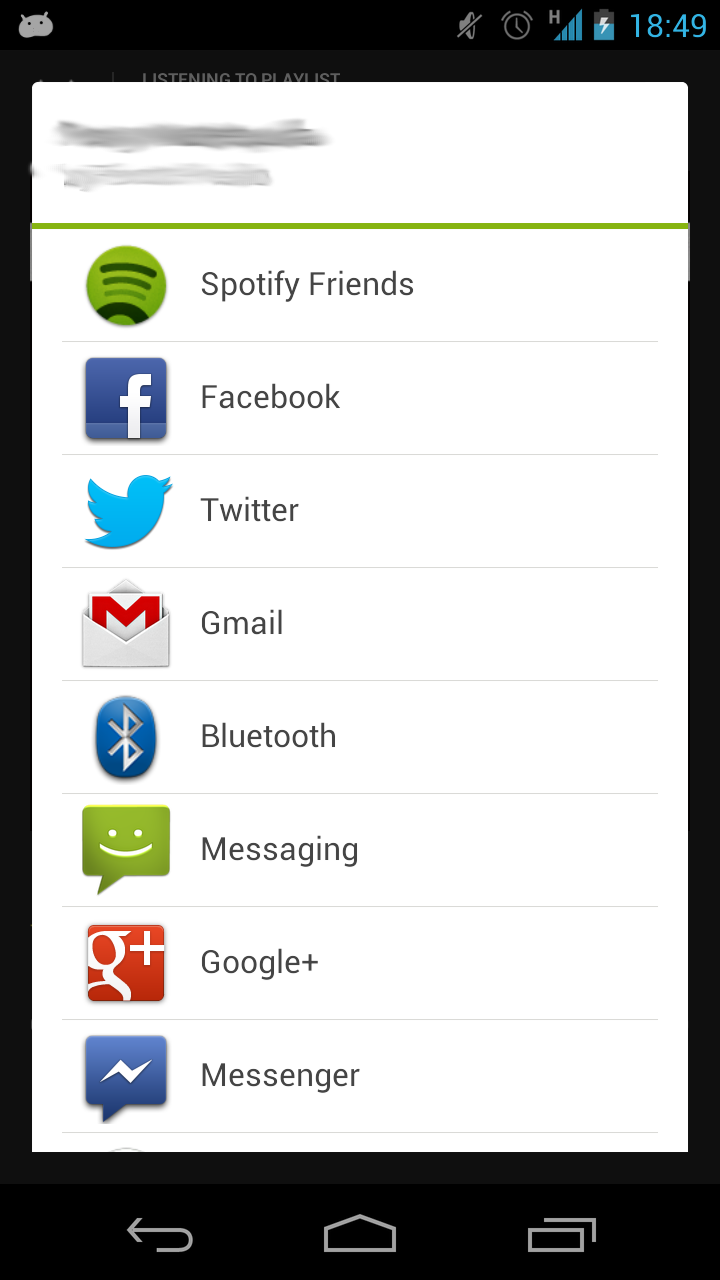
\includegraphics[scale=0.3]{./Android/imagenes/contentProvider.png}
  \caption{Opción compartir de una aplicación.}
  \label{fig:contentProvider}
\end{figure}

\item \textbf{Broadcast Receiver:} es un componente de Android diseñado para actuar cuando ocurre un evento general del sistema, como puede ser la recepción de un SMS, la batería se está agotando, una llamada entrante, etc. También una aplicación puede generar eventos de este tipo para que cualquiera que implemente un Broadcast Receiver pueda recibirlo.

\item \textbf{Widget:} son elementos visuales y generalmente para que el usuario realice alguna acción, tal como poner en pausa la música, pasar de canción, revisar los feed RSS, mirar los correos pendientes, etc. Suele estar en alguna de las pantallas principales de Android. En la figura \ref{fig:widget} podemos ver un widget de GMail.
 
\begin{figure}
  \centering
    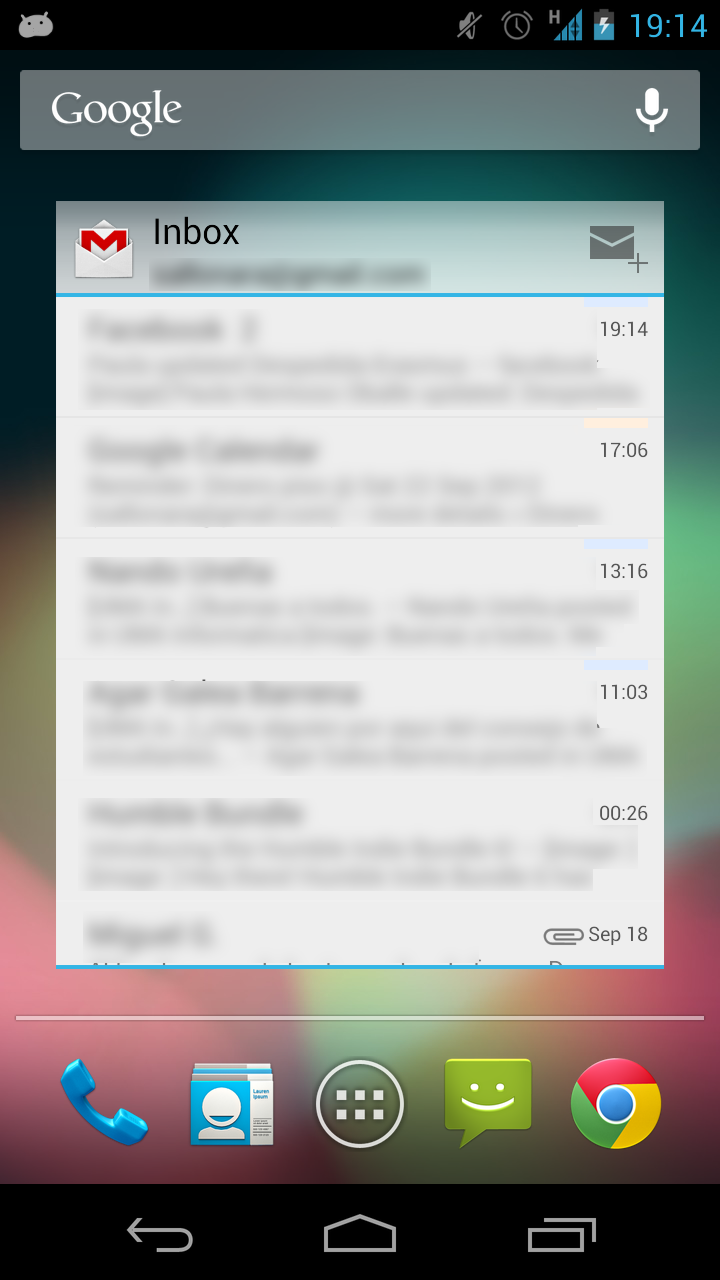
\includegraphics[scale=0.3]{./Android/imagenes/widget.png}
  \caption{Widget de GMail.}
  \label{fig:widget}
\end{figure}

\subsection{Desarrollando en Android.}

%TODO: Poner anexo 
Como ya hemos dicho anteriormente para el desarrollo de la aplicación móvil hemos usado el IDE de programación Eclipse. En el anexo !!!??¿ podemos ver toda la configuración de Eclipse para la programación de aplicaciones Android. En la sección \ref{cap:proyectoBasico} se explicará con más detenimiento la estructura de un proyecto básico en Android.

En este apartado vamos a explicar las entidades más importantes que existen en Android, como pueden ser las activity, fragment, y view usados en el proyecto.

En el proyecto la entidad más importante que hemos usado es la \textbf{activity}. Normalmente las activity están enfocadas a interactuar con el usuario de alguna forma, ya puede ser necesitando de alguna acción del usuario o mostrando información y normalmente ocupando toda la pantalla del teléfono, pero puede flotar dentro de otra activity o agruparse con otras usando la clase \textit{ActivityGroup}. Todas las subclases que hereden de Activity tienen que implementar dos métodos impresindibles. Estos son \textit{onCreate(Bundle)} y \textit{onPause()}. El primero es donde se inicializa la activity y en el segundo es lo que ocurre cuando el usuario abandona la activity.

Habitualmente toda activity tiene una interfáz gráfica que se diseña en un fichero XML, como veremos posteriormente, este archivo se le tiene que indicar a cada activity con el método \lstinline[language=Java]!setContentView(int);! al cual hay que pasarle una constante que genera automáticamente la clase R de Android. Una vez se le ha indicado el archivo XML se puede obtener cada uno de los componentes (botones, cuadros de texto, etc) que componen la intefaz gráfica con el método \lstinline[language=Java]!findViewById(int)!. Todo este proceso se tiene que realizar dentro del método onCreate y se puede observar en el siguiente trozo de código.

\begin{lstlisting}[style=Java]
@Override
protected void onCreate(Bundle savedInstanceState) {
	super.onCreate(savedInstanceState);
	setContentView(R.layout.initialconfigurescreen);

	TextView tAccountOk = (TextView) findViewById(R.id.tAccountOk);
	EditText tCertificate = (EditText) findViewById(R.id.tCertificate);
	ImageView image = (ImageView) findViewById(R.id.imageView1);

	Button bSelectAccount = (Button) findViewById(R.id.bConfigureScreenAccount);
}

\end{lstlisting}


A continuación vamos a explicar las características y su ciclo de vida de las activity, ya que es un tema muy importante cuando desarrollamos una aplicación Android. En la figura \ref{fig:cicloActivity} podemos ver todos los estados por los que pasa una activity desde que se crea hasta que finaliza. 

\begin{figure}
  \centering
    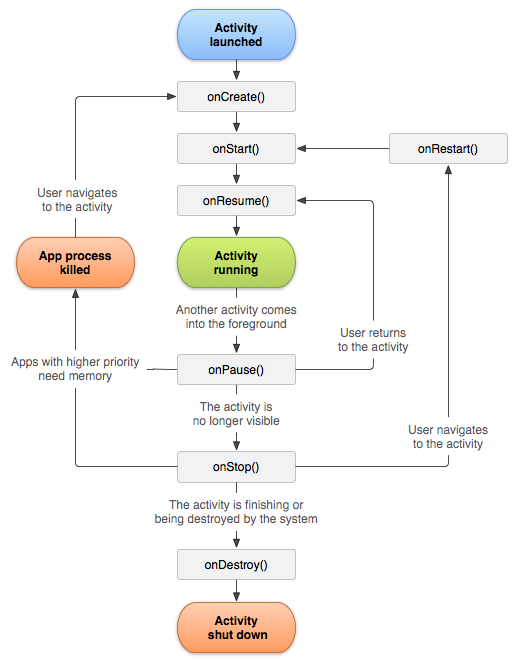
\includegraphics[scale=0.8]{./Android/imagenes/cicloActivity.png}
  \caption{Ciclo de vida de una activity.}
  \label{fig:cicloActivity}
\end{figure}

Todos estos estados se pueden controlar mediantes la implementación de los siguientes métodos.

\begin{lstlisting}[style=Java]
public class Activity extends ApplicationContext {
	protected void onCreate(Bundle savedInstanceState);

	protected void onStart();

	protected void onRestart();

	protected void onResume();

	protected void onPause();

	protected void onStop();

	protected void onDestroy();
}
\end{lstlisting}

Como podemos ver en la figura \ref{fig:cicloActivity} podemos ver que el ciclo completo de una activity es desde el método \lstinline[style=Java]!onCreate(Bundle);! hasta que se realiza la llamada al método \lstinline[style=Java]!onDestroy();!. Como hemos visto antes en \lstinline[style=Java]!onCreate(Bundle);! se genera todo lo necesario para que la activity funcione, como puede ser la inicialización de la interfaz, la creación de un hilo para que realice una operación en background o cualquier otra acción que necesite de una inicialización. El método \lstinline[style=Java]!onDestroy();! se pararía el hilo y se liberá la memoria usada por la activity. Entre los procesos \lstinline[style=Java]!onStart();! y \lstinline[style=Java]!onStop();! es donde se mantienen los recursos para que la activity pueda mostrar los datos al usuario. Por ejemplo si tenemos un BroadcastReceiver que nos puede cambiar la interfaz de usuario pues lo registramos en el método \lstinline[style=Java]!onStart();! y lo paramos en \lstinline[style=Java]!onStop();!. Estos dos métodos se llaman mucho a lo largo de la ejecución de la activity cada vez que el usuario oculta la activity y vuelve a ejecutarla. Los métodos \lstinline[style=Java]!onResume();! y \lstinline[style=Java]!onPause();! se usan para intercambio de activity, cuando apagamos la pantalla del móvil y volvemos a encenderla, cuando giramos la pantalla, etc. En estos métodos se suelen usar Bundles para intercambiar información entre los estados y así conseguir por ejemplo restaurar el texto de un cuadros de texto cuando vuelve a generarse.

En esta tabla podemos observar en cada estado del ciclo de vida de una activity puede ser matada y cual sería el próximo estado.

\begin{tabular}{|l | c | r|}

\hline
Method & ¿Terminable? & Proximo estado\\
\hline
onCreate() & No & onStart()\\
\hline
onRestart() & No & onStart()\\
\hline
onStart() & No & onResume() o onStop()\\
\hline
onResume() & No & onPause()\\
\hline
onPause() & No  & onResume() o onStop()\\
\hline
onStop() & Sí & onRestart() o onDestroy()\\
\hline
onDestroy() & Sí & Ninguna\\
\hline

\end{tabular}

Antes de la versión 3.0 de Android las activity tenian que ocupar toda la ventana y para cambiar o mostrar otra pantalla había que generar una nueva activity de la siguiente forma:

\begin{lstlisting}[style=Java]
Intent intent = new Intent(activity, SplashScreenActivity.class);
startActivity(intent);
\end{lstlisting}

Ese trozo de código se ejecuta en una activity y podemos ver que se crea un objetos Intent al cual se le dice la activity en la que está y la activity que tiene que iniciar, en este caso la variable activity es la actual, y SplashScreenActivity es una activity que tiene la función de inciar todas las variables y realizar las conexiones básicas en el proyecto, acto seguido se usa el procedimiento \lstinline[style=Java]!startActivity(intent);! al que se le pasa el objeto Intent creado anteriormente y con esto tendríamos la nueva activity corriendo.

Desde la versión 3.0 y posteriores las activity siguen ocupando toda la pantalla pero se dio la posibilidad al programador de que usara solo trozos de ella con una clase llamada Fragment de esta forma no tendría que iniciar una nueva activity cada vez que quiera modificar la interfáz, de este modo se pudieron empezar a usar gestos de scroll laterar para mostrar varias interfaces o en pantallas grandes como una tablet poder modificarla sin tener que generar una nueva activity. 

\begin{figure}
  \centering
    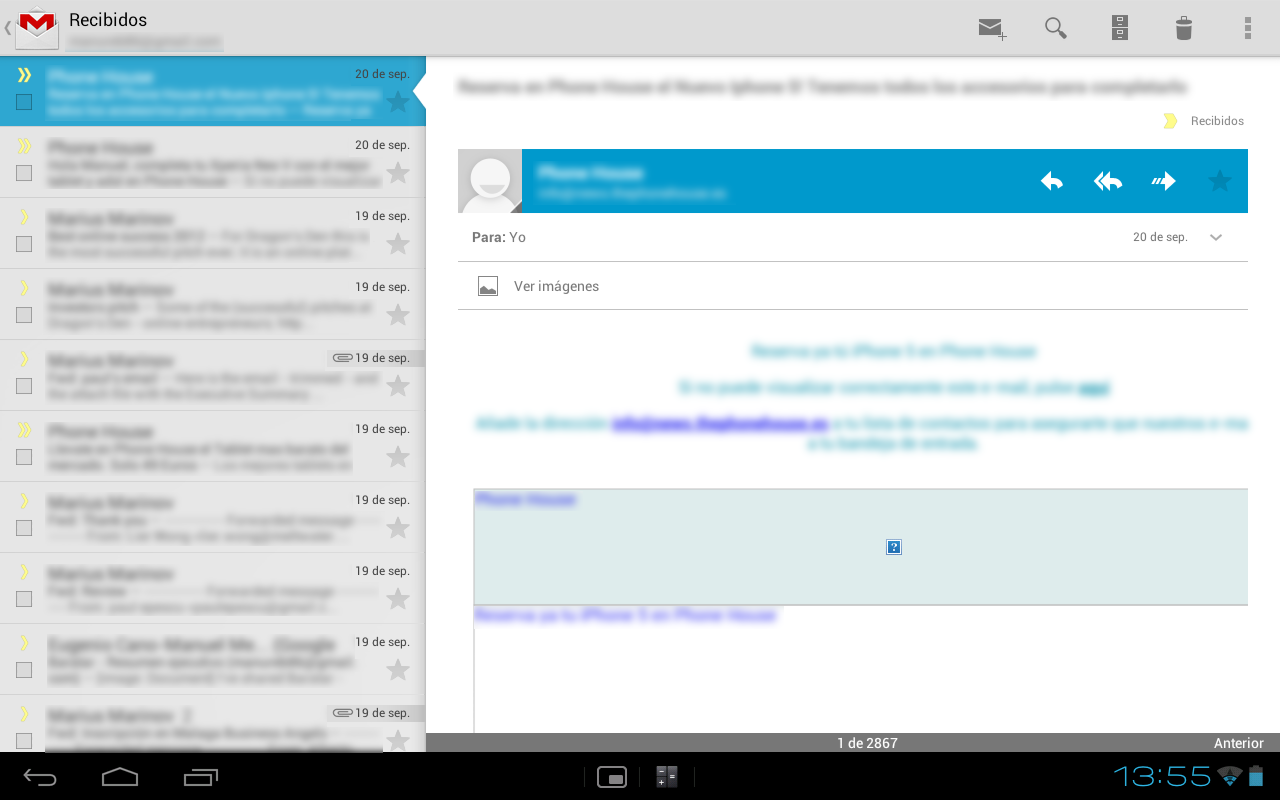
\includegraphics[scale=0.3]{./Android/imagenes/gmailTablet.png}
  \caption{Aplicación de Gmail para tablet.}
  \label{fig:gmailTablet}
\end{figure}

\begin{figure}
  \centering
    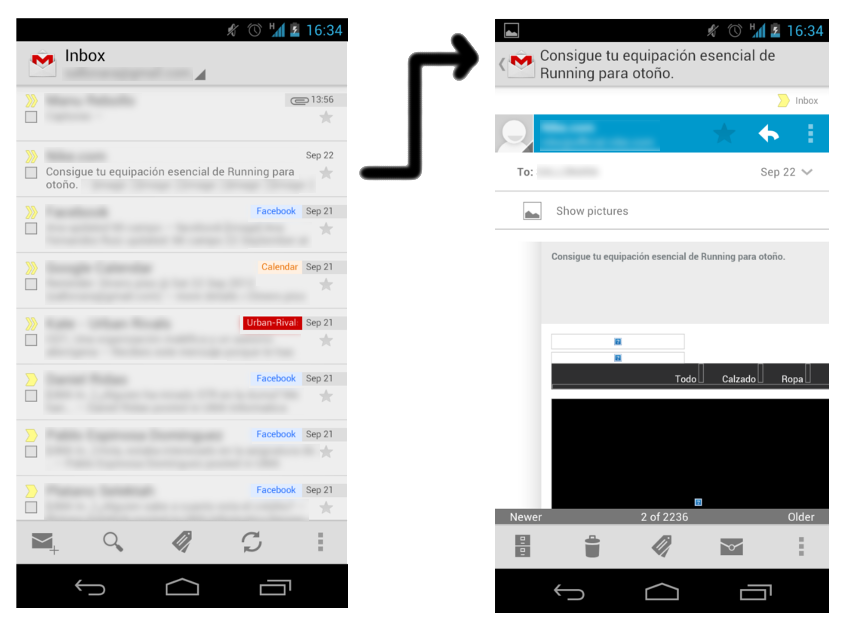
\includegraphics[scale=0.4]{./Android/imagenes/gmailMovil.png}
  \caption{Aplicación de Gmail para móvil.}
  \label{fig:gmailMovil}
\end{figure}

En la imagen \ref{fig:gmailTablet} podemos ver la aplicación de Gmail diseñada mediante fragment y en ella si pulsamos algún correo en la parte izquierda de la aplicación nos mostraría el correo en la derecha sin tener que recagar la aplicación. En la imagen \ref{fig:gmailMovil} podemos ver como en la versión movil no se usa esta forma por falta de espacio en la pantalla. Nosotros hemos realizado un diseño para intercambio de fragment mediante un gesto llamado swype o scroll lateral y como se puede ver en la imagen \ref{fig:swype} podemos ver que no hay que volver a cargar otra activity ni nada, por lo que dotamos a la aplicación de una mayor fluidés.

\begin{figure}
  \centering
    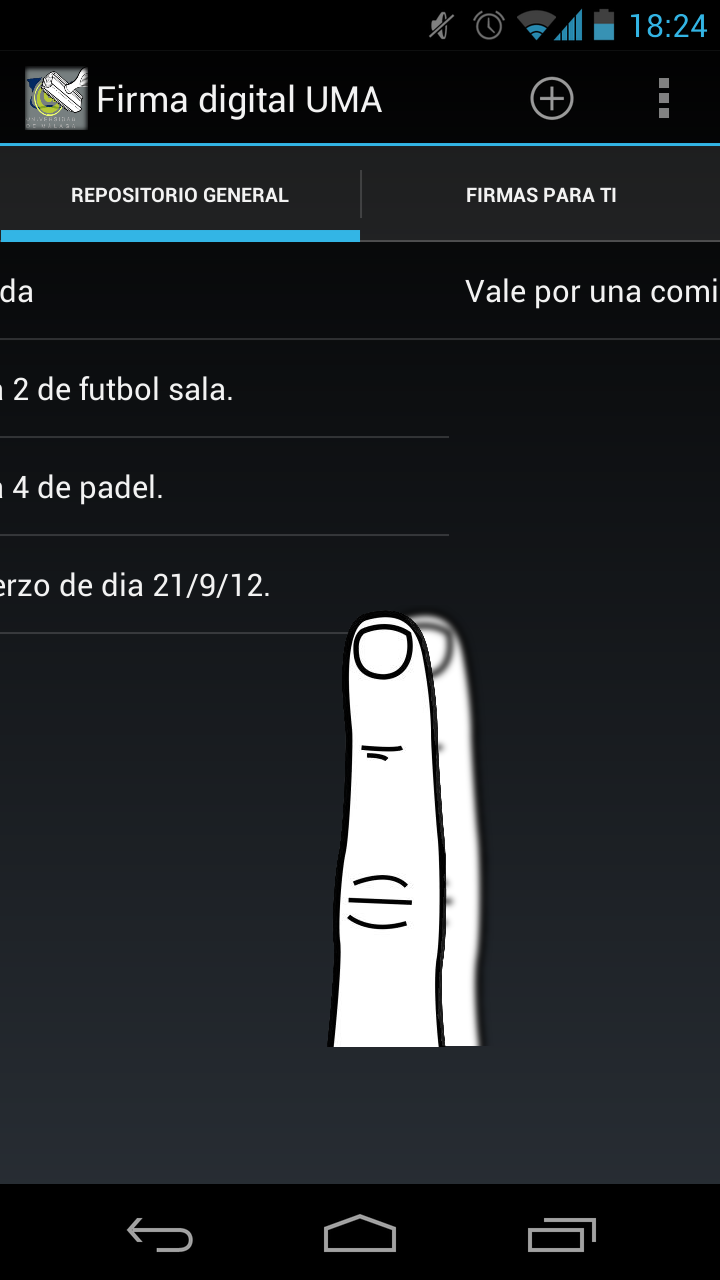
\includegraphics[scale=0.3]{./Android/imagenes/swype.png}
  \caption{Gesto Swype en la aplicación móvil.}
  \label{fig:swype}
\end{figure}

Para que una aplicación pueda usar una determinada activity, el programador primeramente tiene que definir el uso y su función en el archivo \textit{AndroidManifest.xml}. Podemos ver un extracto de dicho archivo donde definimos una de las activities del proyecto.

\begin{lstlisting}[style=XML]
<activity android:name=".FirmaDigitalUMA_ICSActivity" />
<activity android:name=".InitialConfiguration" android:noHistory="true" />
\end{lstlisting}

Se puede observar que hemos declarado dos activities una sin ninguna opción y otra en la que no se guardará en la pila de llamadas de activity, por lo que si pulsamos el botón atrás no se abrirá de nuevo. Si no realizamos este proceso nos dará un error en tiempo de ejución la aplicación diciendo que hemos intentado ejecutar una activity que no está declarada.

\subsection{Proyecto básico de Android en Eclipse.}\label{cap:proyectoBasico}

A continuación vamos explicar con más detenimiento la estructura que tiene un proyecto básico de Android en Eclipse.

\begin{figure}
  \centering
    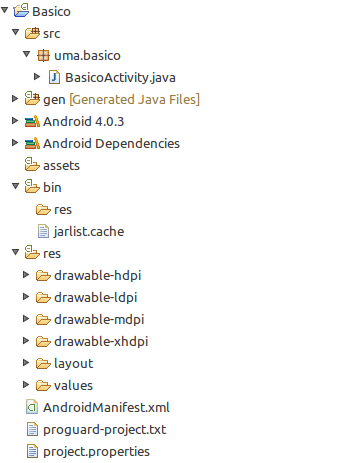
\includegraphics[scale=1]{./Android/imagenes/estructuraBasicaAndroid.png}
  \caption{Estructura básica de un proyecto Android.}
  \label{fig:estructuraBasicaAndroid}
\end{figure}

En la figura \ref{fig:estructuraBasicaAndroid} podemos ver una captura de un proyecto acabado de crear. Podemos observar que se genera una carpeta principal de la que posteriormente colgarán el resto de carpetas necesarias. Estas carpetas son \textit{src}, \textit{gen}, \textit{assets}, \textit{bin}, \textit{res} y varios archivos sueltos como con \textit{AndroidManifest.xml}, \textit{proguard-project.txt}, \textit{project.properties}, vamos a explicar brevemente que contiene y cual es la función de dichas carpetas y documentos.

\begin{itemize}

\item \textbf{src:} en esta carpeta está todo el paquete que contiene los archivos de código fuente que se necesitan en el proyecto.

\item \textbf{gen:} esta carpeta es donde se almacena todo lo que el proyecto de android necesita para funcionar, casi todos los ficheros que se encuentran en el interior se generan cada vez que se construye el proyecto y si los modificamos nosotros cuando volvamos a construir el proyecto borrará todos los cambios. Dentro está la clase R donde se declaran la mayoría de las constantes con direcciones de memoria que luego en tiempo de ejecución se usarán para realizar la conversión en bytecode del archivo java.

\item \textbf{bin:} es una carpeta donde se almacenan todos los archivos binarios, como puede ser el archivo APK, los archivos DEX, etc.

\item \textbf{res:} esta carpeta la encargada de contener todos los recursos necesarios para nuestra aplicación. Esta carpeta se divide en varias, como por ejemplo \textit{drawable-hdpi}, \textit{drawable-ldpi}, \textit{drawable-mdpi}, \textit{drawable-xhdpi} es donde se añaden todas imágenes usadas, sonidos, videos, etc. Pero no todos los recursos son contenido multimedia, hay otras carpetas como por ejemplo la carpeta \textit{layout} donde se almacenan las diferentes interfaces usadas en el en formato XML o la carpeta \textit{values} donde se guardan todas las cadenas constantes en un archivo XML y se pueden usar posteriormente en una interfaz gráfica por ejemplo.

\item \textbf{AndroidManifest.xml:} como ya hemos explicado anteriormente es el archivo donde se declara todos los permisos e información de interes de la aplicación, como pueden ser las activity, los intent, el SDK mínimo que tiene que poseer el móvil para ejecutar nuestra aplicación, etc.  

\item \textbf{proguard-project.txt:} ProGuard es una herramienta que ofrece Google dentro del SDK de Android para ofuscación de código, ya que hay muchas herramientas de ingeniería inversa que mediante la decompilación de los archivos DEX se puede llegar casi a conseguir el código realizado sin permiso. En este archivo se puede configurar los diferentes valores para el uso de esta herramienta, tales como son que tipo de ofuscación queremos utilizar si solo sintáctica o semántica, si queremos que se pueda tracear la salida del archivo, etc. Para amplicar conocimientos sobre dicha herramienta podemos visitar esta web, \url{http://developer.android.com/tools/help/proguard.html} donde está toda la información necesaria.

\item \textbf{project.properties:} es un archivo donde se pueden configurar diferentes parámetros del proyecto, como puede ser la API sobre la que se va a ejecutar el proyecto, o si queremos usar una herramienta que ofrece Google dentro del SDK para ofuscar el código llamada ProGuard.
\end{itemize}

\section{Proyecto firma digital UMA.}

La aplicación Firma digital UMA es la aplicación móvil que hemos realizado para facilitar la visualización y firma de nuevos documentos. En ella  podemos comprobar los documentos anteriormente firmados o firmar nuevos de una forma fácil, el resto de gestión se tiene que realizar desde la aplicación web, donde se puede verificar, generar nuevos documentos, etc. En la figura~\ref{fig:pantallaPrincipal} podemos ver el aspecto de la aplicación.

\begin{figure}
  \centering
    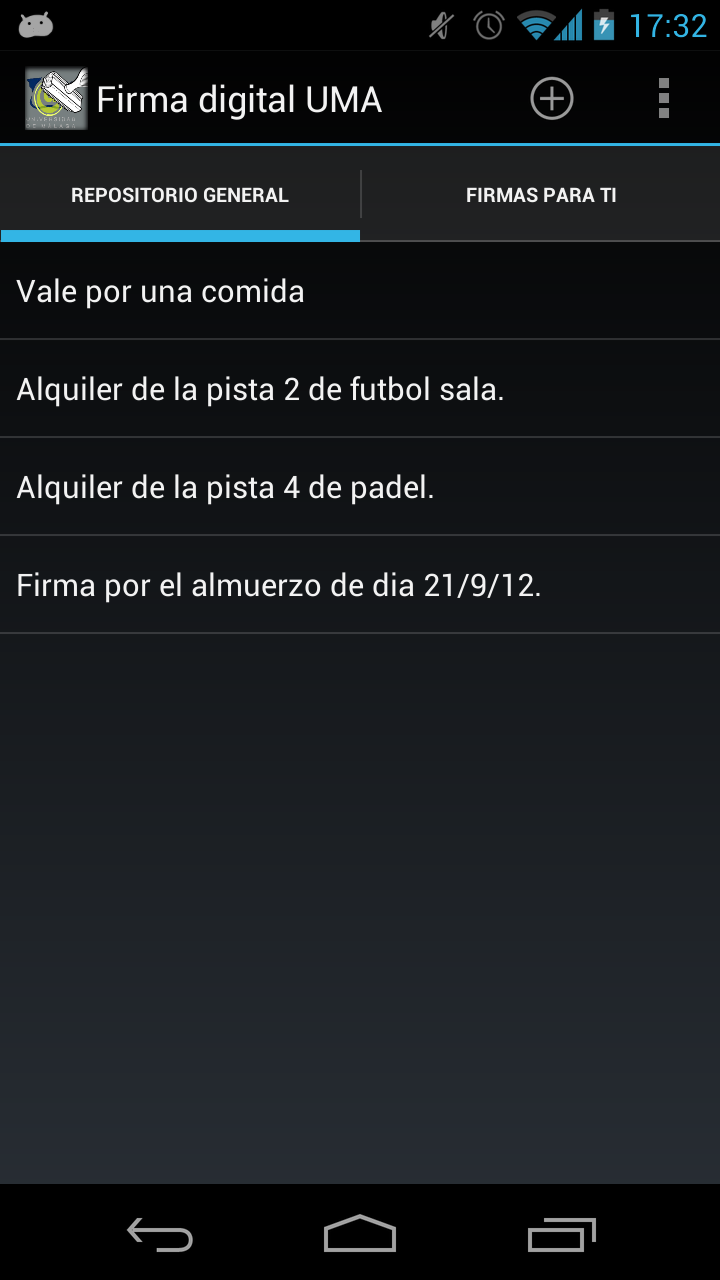
\includegraphics[scale=0.3]{./Android/imagenes/pantallaPrincipal.png}
  \caption{Pantalla inicial de la aplicación.}
  \label{fig:pantallaPrincipal}
\end{figure}

\subsection{Uso de la aplicación.}

Lo primero que pensamos cuando nos pusimos a diseñar la aplicación era que el método se firma tiene que ser rápido y fácil, por lo que se decidió usar los códigos QR para agilizar la lectura de información. Solo hay que pulsar el botón de añadir nuevo recibo (figura~\ref{fig:botonAnhadir}) y se abrirá el lector de códigos QR, una vez leidos el código este se firmará y se subirá automaticamente al servidor sin necesitar que el usuario realice otra acción.

\begin{figure}
  \centering
    
\includegraphics[scale=0.3]{./Android/imagenes/botonAnhadir.png}
  \caption{Detalle del botón añadir.}
  \label{fig:botonAnhadir}
\end{figure}

La aplicación se puede dividir principalmente en dos partes claramente diferenciadas, una en la que se muestra las firmas realizadas y otra en la que se muestran que tienen como destino el usuario que está ejecutando la aplicación. Las dos partes son practicamente idénticas y tienen el mismo uso. Si pulsamos encima de cualquier recibo de la lista nos mostrará toda la información de dicha firma, podemos ver un ejemplo en la figura~\ref{fig:informacionFirma}. Podemos observar todos los datos necesarios, como pueden ser destino, quien la ha mandado, la fecha, el texto, etc y también podemos ver si está verificada con el tick de color verde o una señal de error roja si no está verificada, que podemos ver en la esquina superior derecha. En el caso de los recibos de los cuales se es recipiente se pone de una forma más clara quien es el que usuario que envia el mensaje pero el resto de la información es la misma. En la información que nos proporcionan podemos ver la dirección del servidor de tiempo usado y si pulsamos en ella se abrirá el navegador con una dirección donde podremos confirmar el hash y la fecha en la que se realizó la firma.

\begin{figure}
  \centering
    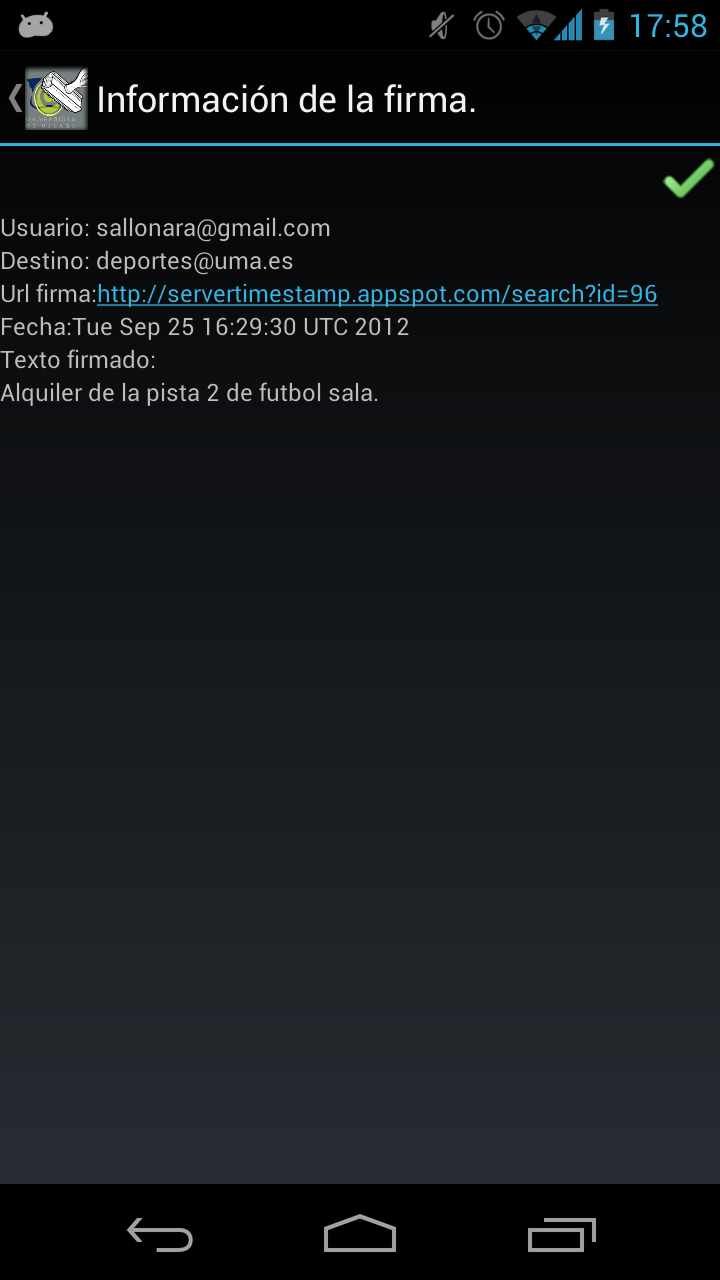
\includegraphics[scale=0.3]{./Android/imagenes/informacionFirma.png}
  \caption{Información de una firma realizada.}
  \label{fig:informacionFirma}
\end{figure}

\subsection{Explicación del proyecto de Android.}

En la figura~\ref{fig:proyectoAndroid} podemos ver el proyecto de eclipse con todas las clases que hemos tenido que desarrollar, desde la conexión a la base de datos, el inicio de la aplicación, el cifrado, etc. La estructura del proyecto es la misma que ya hemos explicado anteriormente.

\begin{figure}
  \centering
    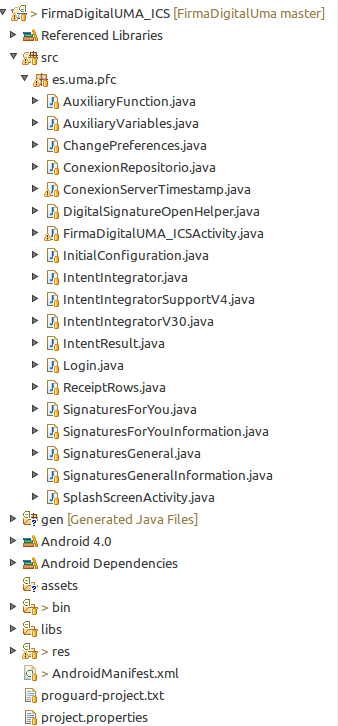
\includegraphics[scale=0.7]{./Android/imagenes/proyectoAndroid.png}
  \caption{Proyecto de android en Eclipse.}
  \label{fig:proyectoAndroid}
\end{figure}

A continuación vamos a explicar cada una de las clases y la función que tiene dentro del proyecto.

\begin{itemize}

\item \textbf{AuxiliaryFunction.java:} en esta clase se han implementado todas las funciones que son usadas muchas veces en el proyecto, como puede ser la función que verifica si un certificado existe en un path determinado y si se puede abrir, también está la función que pasa de un array de bytes a una cadena de texto. 

\item \textbf{AuxiliaryVariables.java:} aquí se almacenan todas las variables comunes que vamos a necesitar para que la aplicación funcione correctamente. En el siguiente trozo de código podemos ver que son variables como el login con el cual se está logueado, la cookie para autentificación en el servicio, el key store con las claves para realizar las firmas, si la aplicación está sin internet para mostrar la base de datos que tengamos almacenados y no intentar bajar recibos nuevos y otras.

\begin{lstlisting}[style=Java]
private static Login LOGIN_GLOBAL;
private static Cookie COOKIE_GLOBAL;
private static KeyStore KEYSTORE_GLOBAL;
private static boolean WITHOUT_INTERNET;
private static List<ReceiptRows> LIST_RECEIPT;
private static String THEME;
\end{lstlisting}

Además de las variables tenemos todos los getter and setter de las variables.

\item \textbf{ChangePreferences.java:} esta clase es la encargada de realizar todo el manejo del cambio de preferencias si se produce. En la aplicación hemos usado una clase que proporciona android para el almacenado de configuración llamada SharedPreferences, al usar este método android proporciona listener para que cuando cambien se activen, de esta forma podemos controlar todos los cambios que realicemos actualizando en el acto la interfaz y guardando los datos en el acto. Un trozo de la clase en el que se puede observar como se crea y se implementa un listener para cuando se produzca un cambio en la configuración podamos actualizar tanto las shared preferences como la interfaz.

\begin{lstlisting}[style=Java]
EditTextPreference textPath = (EditTextPreference) findPreference(getActivity().getResources().getString(R.string.key_cert_path));

// Para que cuando cambie el texto lo cambie también en el título...
textPath.setOnPreferenceChangeListener(new OnPreferenceChangeListener() {
	public boolean onPreferenceChange(Preference preference, Object newValue) {
		EditTextPreference textPath = (EditTextPreference) preference;
		String s = (String) newValue;

		String pass = settings.getString("certificate_password", "NotValue");
		if (!pass.equals("NotValue")) {
			boolean check = AuxiliaryFunction.checkCert(s, pass);

			if (check) {
				textPath.setSummary(s);
				textPath.setText(s);
				Editor editor = settings.edit();
				editor.putString("path_certificate", s);
				editor.commit();
				return true;
			} else {
				textPath.setSummary("No se ha podido cargar el certificado,\nla ruta no es correcta");
				return true;
			}
		} else {
			textPath.setSummary("Password no guardado");
			return true;
		}

	}

});
\end{lstlisting}

Creamos la variable EditTextPreference donde mostraremos el password del certificado que estamos usando para firmar el texto. A continuación implementamos el listener OnPreferenceChangeListener, el cual se activará cuando digamos de cambiar el password del certificado. Podemos observar que cuando introducimos un nuevo password hacemos una comprobación para ver si después del cambio podemos seguir usando dicho certificado, si no es posible informamos al usuario diciendole que no se ha guardado el password.

\item \textbf{ConexionRepositorio.java:} en esta clase se ha implementado todo lo referente a interactuar con la aplicación web repositorio general. En dicha clase se ha implementado el método para añadir un recibo nuevo, listar todos los recibos que hay guardados, etc. Todos los métodos son estáticos para no tener que crear instancias de esta clase, además se vio que teníamos que crear una nueva conexión cada vez que queríamos añadir un nuevo nuevo recibo, por lo que no tendría sentido crea instancias de la clase. A continuación podemos ver el método que añade un nuevo recibo.

\begin{lstlisting}[style=Java]
public static String addRow(String plainText, String tokenTime, Account account, String to) {
	/*
	 * Primero se le codifican los espacios porque si no la función
	 * URLEncoder.encode los cambia por '+' y si el documento tiene '+'
	 * luego los pone como si fueran espacios
	 */
	String textoSinEspacios = plainText.replace(" ", "%20");
	textoSinEspacios = URLEncoder.encode(textoSinEspacios);
	String token = tokenTime.split(";;")[1];
	String fecha = tokenTime.split(";;")[2];
	String url = cadServer + cadAdd + cadServerTimestampSearch + token + "&texto=" + textoSinEspacios + "&token=" + token + "&usuario=" + account.name
			+ "&destino=" + to + "&fecha="+ fecha;
	String response = "";
	try {
		URL u1 = new URL(url);

		// Si queremos usar el proxy inicializarlo de esta forma, donde
		// sa es: SocketAddress sa = new
		// InetSocketAddress("proxy.alu.uma.es", 3128);
		// HttpURLConnection c = (HttpURLConnection)
		// u.openConnection(new Proxy(Proxy.Type.HTTP, sa));

		Cookie cookie = AuxiliaryVariables.getCOOKIE_GLOBAL();
	
		HttpURLConnection con1 = (HttpURLConnection) u1.openConnection();

		con1.addRequestProperty("Cookie", cookie.getName() + "=" + cookie.getValue());
		con1.setRequestMethod("GET");
		con1.connect();

		DataInputStream is1 = new DataInputStream(con1.getInputStream());
		response = is1.readLine();

		con1.disconnect();

	} catch (MalformedURLException e) {
		response = "MalformedURL";
		e.printStackTrace();
	} catch (ProtocolException e) {
		response = "ProtocolException";
		e.printStackTrace();
	} catch (IOException e) {
		response = "IOException";
		e.printStackTrace();
	}
	return response;
}
\end{lstlisting}

La función necesita una serie de parámetros para poder ser invocada, estos parámetros son los datos que necesitamos almacenar, como pueden ser el texto en claro, el token de tiempo que ha devuelto la aplicación web de timestamp, la cuenta con la que se está usando la aplicación y el destino, el resto de valores o los añade la aplicación web o la aplicación del móvil. A continuación se realiza la conexión con el servidor y se recibe una cadena donde se indica si se ha realizado bien la operación.

\item \textbf{ConexionServerTimestamp.java:} al igual que la clase anterior en esta se ha realizado todo lo relacionado con la aplicación web del servidor timestamp. Solo tiene una función que es la de añadir al servidor que tiene un aspecto similar a la mostrada en el apartado anterior.

\item \textbf{DigitalSignatureOpenHelper.java:} esta clase es la encargada de la creación de la base de datos SQLite, cuando vamos a necesitar tener acceso a ella hay que generar un objeto de dicha clase y llamar al contructor, que devuelve un objeto con el que podremos insertar, buscar o borrar elementos de la base de datos. Al pensar en el diseño de la aplicación se creyó necesario el uso de la base de datos para almacenar todos los recibos que se han realizado hasta la fecha, la aplicación sabe cual es el último recibo que tiene almacenado y solo pide a la aplicación web que le de los recibos nuevos, de esta forma de ahorra en tiempo de inicio de la aplicación y además en la cantidad de datos móviles que usamos.

Esta clase tiene que heredar de SQLiteOpenHelper que es la clase genérica que proporciona Android para manejo de la base de datos SQLite que tiene. Hay que implementar el constructor y dos métodos más obligatoriamente \lstinline{public void onCreate(SQLiteDatabase db);} y \lstinline{public void onUpgrade(SQLiteDatabase db, int oldVersion, int newVersion);}, el primero es usado para crear la base de datos en la primera ejecución y el segundo para actualizar la base de datos cuando sea necesario.

La base de datos se crea que con la siguiente sentencia SQL, podemos verla en el siguiente listado.

\begin{lstlisting}[style=Java]
static final String KEY_SEQ_NUM = "NUM_SEC";
static final String KEY_SIGN_URL = "URL_FIRMA";
static final String KEY_PLAIN_TEXT = "TEXTO_CLARO";
static final String KEY_TIME_TOKEN = "TOKEN_TIEMPO";
static final String KEY_USER = "USUARIO";
static final String KEY_VERIFY = "VERIFICADO";
static final String KEY_DESTINY = "DESTINO";
static final String KEY_DATE = "FECHA";

private static final String DIGITALSIGNATURE_TABLE_CREATE = "CREATE TABLE " + DIGITALSIGNATURE_TABLE_NAME + " (" +
	BaseColumns._ID + " INTEGER PRIMARY KEY AUTOINCREMENT," +
	KEY_SEQ_NUM + " TEXT, " +
	KEY_SIGN_URL + " TEXT, " +
	KEY_PLAIN_TEXT + " TEXT, " +
	KEY_TIME_TOKEN + " TEXT, " +
	KEY_USER + " TEXT, " +
	KEY_VERIFY + " TEXT, " +
	KEY_DESTINY + " TEXT, " +
	KEY_DATE + " TEXT );";
\end{lstlisting}

\item \textbf{FirmaDigitalUMA\_ICSActivity.java:} esta es la clase principal del proyecto, en ella se crea la activity principal de la aplicación. Se puede ver en el código que no extiende a la clase \lstinline{Activity}, si no que lo hace de \lstinline{FragmentActivity}, esto es así porque como ya hemos explicado anteriormente se han usado fragment para el diseño de la aplicación y no solo activitys. Además de esto se ha añadido funcionalidad mediante el uso de \lstinline{ViewPager} y \lstinline{TabsAdapter}, el primero para el uso del scroll lateral y el segundo para tener las dos pestañas de los recibos que el usuario a firmado y de los que es recipiente. En el siguiente trozo de código podemos ver la creación de los dos elementos que hemos dicho antes, junto con la action bar.

\begin{lstlisting}[style=Java]
mViewPager = new ViewPager(this);
mViewPager.setId(R.id.pager);
setContentView(mViewPager);

final ActionBar bar = getActionBar();
bar.setTitle("Firma digital UMA");
bar.setNavigationMode(ActionBar.NAVIGATION_MODE_TABS);

mTabsAdapter = new TabsAdapter(this, mViewPager);
mTabsAdapter.addTab(bar.newTab().setText("Repositorio general"), SignaturesGeneral.class, null);
mTabsAdapter.addTab(bar.newTab().setText("Firmas para ti"), SignaturesForYou.class, null);
\end{lstlisting}

Además de la creación de los elementos anteriores esta clase también es la encargada de crear los menús, que en la versión 4.0 de android tienden a desaparecer, debido a la desapareción del botón menú de los nuevos terminales, pero que en las nuevas versión se añade a la action bar. A continuación podemos ver como se crean y añaden los botones de añadir un nuevo recibo, el de configuración o el de salir de la aplicación.

\begin{lstlisting}[style=Java]
@Override
public boolean onCreateOptionsMenu(Menu menu) {
	MenuInflater inflater = getMenuInflater();
	inflater.inflate(R.menu.main, menu);
	return true;
}
@Override
public boolean onOptionsItemSelected(MenuItem item) {
	switch (item.getItemId()) {

	case R.id.menuitem_add:
		Log.d(AuxiliaryVariables.TAG_DEBUG, "Add");
		IntentIntegrator intentQR = new IntentIntegrator(this);
		intentQR.initiateScan();
		return true;

	case R.id.menuitem_quit:
		Log.d(AuxiliaryVariables.TAG_DEBUG, "Quit");
		finish();
		return true;
	case R.id.menuitem_about:
		Log.d(AuxiliaryVariables.TAG_DEBUG, "About");
		Toast.makeText(context, "about", Toast.LENGTH_SHORT).show();
		return true;
	case R.id.menuitem_settings:
		Log.d(AuxiliaryVariables.TAG_DEBUG, "Settings");
		Toast.makeText(context, "ajustes", Toast.LENGTH_SHORT).show();
		Intent prefsIntent = new Intent(getApplicationContext(),
		        ChangePreferences.class);
		startActivity(prefsIntent);
		return true;
	}
	return false;
}
\end{lstlisting}

Además de la creación de la activity y de los menús es la encargada de llamar a la función de subir un recibo a la aplicación web después de recibir por medio de un intent el resultado de la lectura del código QR, se puede observar en este trozo de código.

\begin{lstlisting}[style=Java]
public void onActivityResult(int requestCode, int resultCode, Intent intent) {
	IntentResult scanResult = IntentIntegrator.parseActivityResult(requestCode, resultCode, intent);
	String plaintext = "";
	if ((plaintext = scanResult.getContents()) != null) {
		progressDialog = new ProgressDialog(activity);
		progressDialog.setMessage("Subiendo el recibo...");
		progressDialog.show();

		ConexionRepositorio.addRow(handler, plaintext);
		
	}
}
\end{lstlisting} 

\item \textbf{InitialConfiguration.java:} esta clase es la activity que se encarga de realizar la configuración de la aplicación cuando es la primera ejecución en un teléfono, en ella se tiene que configurar el certificado y su password y la cuenta. Es la encargada de crear las shared preferences para que la aplicación funcione correctamente. %TODO: poner una imagen de esto y revisarlo porque era mu cutre...

\item \textbf{InitialConfiguration.java, IntentIntegratorSupportV4.java, IntentIntegratorV30.java, IntentResult.java:} estas clases son las encargadas de la lectura de los códigos QR. Están hechas por ZXing y se distribuyen bajo licencia Apache License, Version 2.0. Proporcionan mediante un intent la posibilidad de lectura de códigos QR con su aplicación Barcode Scanner (figura~\ref{fig:barcodeScanner}) gratuita en Google Play, si no se tiene la aplicación instalada proporciona los métodos para hacerlo.
\end{itemize}

\begin{figure}
  \centering
    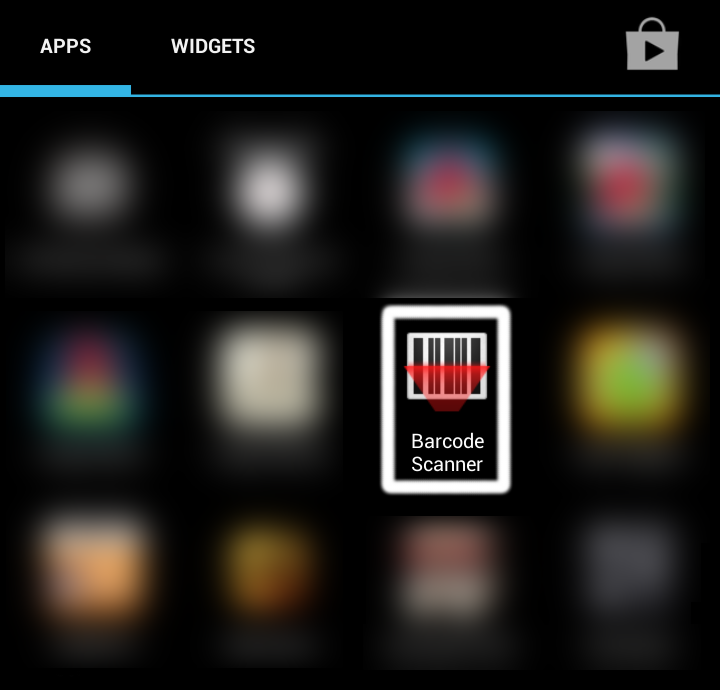
\includegraphics[scale=0.3]{./Android/imagenes/barcodeScanner.png}
  \caption{Aplicación Barcode Scanner.}
  \label{fig:barcodeScanner}
\end{figure}

\begin{itemize}
\item \textbf{Login.java:} esta clase es la encargada de realizar el login en la aplicación web Repositorio General. Google proporciona un método de login si se tienen las credenciales, cosa que tenemos gracias a que en Android se necesita tener una cuenta de Google para poder usar Google Play y los diferentes servicios que ofrece. La dirección a la que tenemos que dirigirnos es a: \url{https://repositoriorecibos.appspot.com/\_ah/login}. Esta clase tiene una variable privada que es el token de autentificación que conseguimos mediante la realización del login, para conseguirlo mostramos todas las cuentas de Google que hay configuradas en el terminal Android, cuando el usuario selecciona una de ellas iniciamos la conexión con el servidor y recibimos el token. Esto se hace todo el segundo plano para que la aplicación no se quede parada mientras se va a la página web y se consigue el token. En el código que sigue podemos ver el proceso de obtención del token.

\begin{lstlisting}[style=Java]
Thread t = new Thread() {
	public void run() {
		try {
			AccountManagerFuture<Bundle> future = manager.getAuthToken(account, "ah", null, activity, null, null);
			Bundle bundle;
			bundle = future.getResult();
			token = bundle.getString(AccountManager.KEY_AUTHTOKEN);
		} catch (OperationCanceledException e) {
			e1.printStackTrace();
		} catch (AuthenticatorException e) {
			e1.printStackTrace();
		} catch (IOException e) {
			e1.printStackTrace();
		}
	}
}.start();
\end{lstlisting} 

La parte mas interesante del código es en la llamada \lstinline{manager.getAuthToken(account, "ah", null, activity, null, null);} con esta función conseguimos la cookie donde está el token de acceso para posteriormente con la función \lstinline{bundle.getString(AccountManager.KEY_AUTHTOKEN);} conseguirlo.

La función \lstinline{public Cookie getAuthCookie(String authToken);} se puede ver en el siguiente trozo de código.

\begin{lstlisting}[style=Java]
public Cookie getAuthCookie(String authToken) throws ClientProtocolException, IOException {
	DefaultHttpClient httpClient = new DefaultHttpClient();
	Cookie retObj = null;
	String cookieUrl = gaeAppLoginUrl + "?continue=" + URLEncoder.encode(gaeAppBaseUrl, "UTF-8") + "&auth=" + URLEncoder.encode(authToken, "UTF-8");
	
	HttpGet httpget = new HttpGet(cookieUrl);
	HttpResponse response = httpClient.execute(httpget);
	if (response.getStatusLine().getStatusCode() == HttpURLConnection.HTTP_OK
			|| response.getStatusLine().getStatusCode() == HttpURLConnection.HTTP_NO_CONTENT) {

		if (httpClient.getCookieStore().getCookies().size() > 0) {
			retObj = httpClient.getCookieStore().getCookies().get(0);
		}

	}

	return retObj;
}
\end{lstlisting} 

En ella podemos ver que hacemos una conexión a la dirección \url{http://repositoriorecibos.appspot.com/\_ah/login?continue=http://repositoriorecibos.appspot.com&auth=token}, en la que se le indica el token de acceso y la url a la que tenemos que seguir cuando se realice el login. Una vez realizada la identificación devolvemos la cookie donde irá el token de acceso.

\item \textbf{ReceiptRows.java:} esta clase es la que representa un recibo, con ella se pueden crear objetos para almacenar todos los valores que necesitamos para tener un recibo identificado, como pueden ser el texto, la url de la firma, la fecha, el destino, etc. Este es el tipo de objeto que se usa para recoger la información de la base de datos y para almacenarla. Durante toda la ejecución de la aplicación tedremos una lista de objetos de esta clase para tener acceso a los recibos. Es una clase simple con un contructor con todos los valores que se guardan como parámetros y todos los getter y setter de las diferentes variables. También tiene definidas todas las constantes para el nombre de la tabla de la base de datos.

\item \textbf{SignaturesGeneral.java:} esta clase extiende a \lstinline{ListFragment}, es la lista de los recibos que el usuario a firmado. Es una de las dos pantallas principales de la aplicación, se puede ver en la figura~\ref{fig:signaturesGeneral}. Cuando se genera la interfaz se hace una consulta a la base de datos y se recibe un objeto de la clase \lstinline{Cursor}, en el cual se puede iterar para conseguir todos los recibos que has firmado. En el siguiente trozo de código podemos ver como se hace.
\begin{lstlisting}[style=Java]
DigitalSignatureOpenHelper digitalSignatureOpenHelper = new DigitalSignatureOpenHelper(activity);
	SQLiteDatabase sqLiteDatabase = digitalSignatureOpenHelper.getReadableDatabase();
	Cursor cursor = sqLiteDatabase.query(DigitalSignatureOpenHelper.DIGITALSIGNATURE_TABLE_NAME,
			new String[] { DigitalSignatureOpenHelper.KEY_PLAIN_TEXT }, null, null, null, null, null);
\end{lstlisting} 

\end{itemize}

\begin{figure}
  \centering
    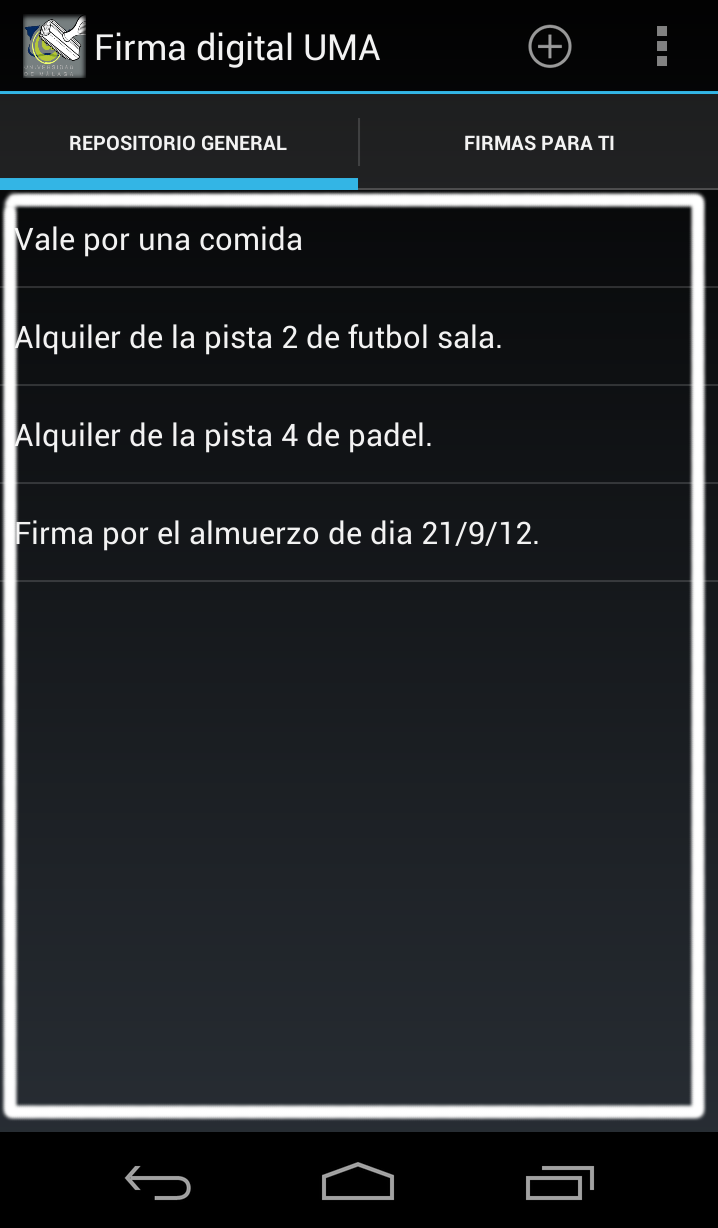
\includegraphics[scale=0.3]{./Android/imagenes/signaturesGeneral.png}
  \caption{Detalle fragment generado por la clase SignaturesGeneral.java.}
  \label{fig:signaturesGeneral}
\end{figure}

\begin{itemize}

\item \textbf{SignaturesGeneralInformation.java:} esta clase es la encargada de mostrar la información cuando pulsamos en algún recibo que hemos firmado. Es una clase que extiende de la clase \lstinline{Activity} y es la encargada de cargar la interfaz modelada en el XML \lstinline{signaturesgeneralinfo.xml} y mostrar toda la información del recibo que ha sido pulsado de la lista de recibos. Cuando se pulsa un recibo en la pantalla anterior que es la generada por \lstinline{SignaturesGeneral.java}, antes de cargar esta se le manda la posición que ha sido pulsada para después poder localizarla y acto seguido se muestra la información, esto se hace por medio de un \lstinline{Intent} al cual se le añade un valor entero con la posición. En el siguiente trozo de código podemos ver se recupera el valor, se realiza la consulta en la base de datos y se rellenan todos los campos donde mostraremos la información del recibo seleccionado.

\begin{lstlisting}[style=Java]
super.onCreate(savedInstanceState);
setContentView(R.layout.signaturesgeneralinfo);

Intent intent = this.getIntent();
int pos = intent.getExtras().getInt("position");

DigitalSignatureOpenHelper digitalSignatureOpenHelper = new DigitalSignatureOpenHelper(this);
SQLiteDatabase sqLiteDatabase = digitalSignatureOpenHelper.getReadableDatabase();
Cursor cursor = sqLiteDatabase.query(DigitalSignatureOpenHelper.DIGITALSIGNATURE_TABLE_NAME, new String[] { DigitalSignatureOpenHelper.KEY_USER,
		DigitalSignatureOpenHelper.KEY_DESTINY, DigitalSignatureOpenHelper.KEY_SIGN_URL, DigitalSignatureOpenHelper.KEY_PLAIN_TEXT,
		DigitalSignatureOpenHelper.KEY_VERIFY, DigitalSignatureOpenHelper.KEY_DATE }, null, null, null, null, null);

if (cursor.moveToPosition(pos)) {
	
	final ActionBar bar = getActionBar();
	bar.setTitle("Información de la firma.");
	bar.setDisplayHomeAsUpEnabled(true);

	TextView textUser = (TextView) findViewById(R.id.text_sign_general_user);
	TextView textDestiny = (TextView) findViewById(R.id.text_sign_general_to);
	TextView textUrl = (TextView) findViewById(R.id.text_sign_general_url);
	TextView textPlainText = (TextView) findViewById(R.id.text_sign_general_plain_text);
	ImageView imageVerify = (ImageView) findViewById(R.id.image_sign_general_verify);
	TextView textDate = (TextView) findViewById(R.id.text_sign_general_date);
	
	textUser.setText(textUser.getText() + " " + cursor.getString(0));
	textDestiny.setText(textDestiny.getText() + " " + cursor.getString(1));
	textUrl.setText(cursor.getString(2));
	textPlainText.setText(cursor.getString(3));

	String verify = cursor.getString(4);
	if (verify.equals("true")) {
		imageVerify.setImageResource(R.drawable.ok);
	} else {
		imageVerify.setImageResource(R.drawable.cancel);
	}
	textDate.setText(cursor.getString(5));

	sqLiteDatabase.close();
}
\end{lstlisting} 

Podemos ver como se genera el objeto \lstinline{DigitalSignatureOpenHelper} y se realiza la consulta con el método \lstinline{public Cursor query (String table, String[] columns, String selection, String[] selectionArgs, String groupBy, String having, String orderBy);}, a continuación generamos todos los \lstinline{TextView} necesarios para mostrar la información y los rellenamos con los datos.

\item \textbf{SignaturesForYou.java:} igual que su clase equivalente \lstinline{Signatures General.java} es la encargada de mostrar una lista con todos los recibos de los que se es destinatario, la estructura es practicamente idéntica, con solo una diferencia y es que se realiza un filtrado para que el campo destino sea el mismo que la cuenta de usuario usada en la aplicación. Podemos ver el resultado en la figura~\ref{fig:signaturesForYou}.

\end{itemize}

\begin{figure}
  \centering
    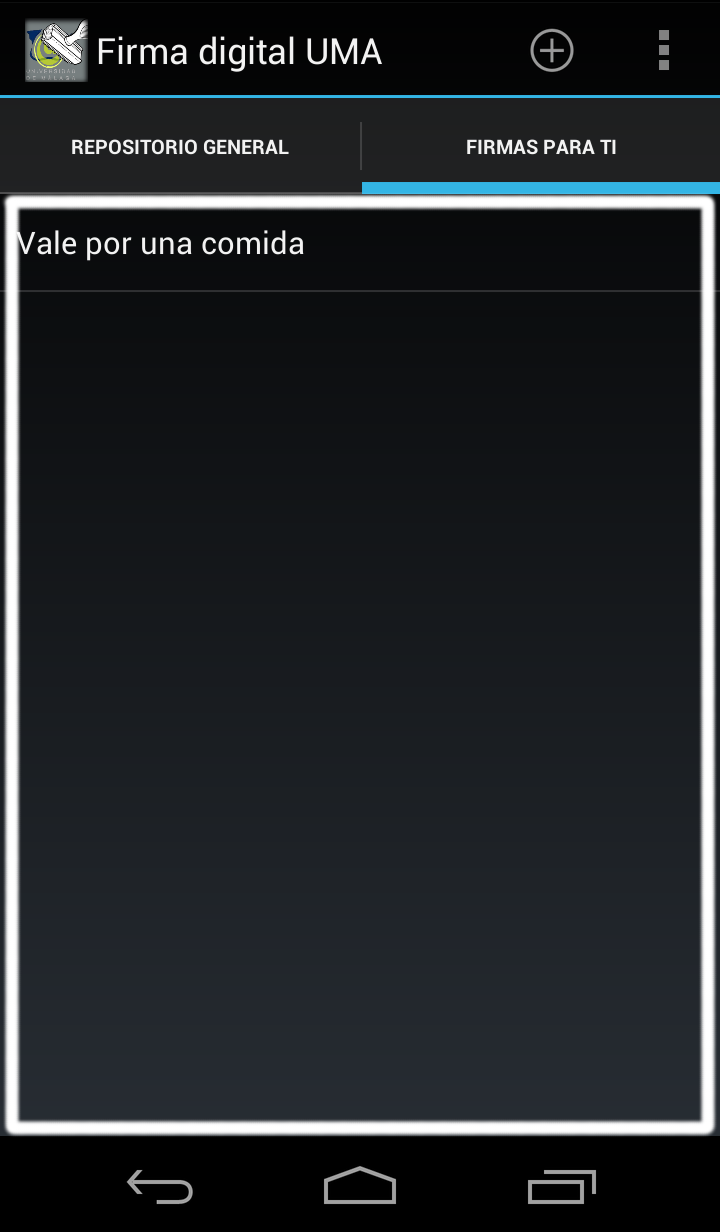
\includegraphics[scale=0.3]{./Android/imagenes/signaturesForYou.png}
  \caption{Detalle fragment generado por la clase SignaturesForYou.java.}
  \label{fig:signaturesForYou}
\end{figure}

\begin{itemize}

\item \textbf{SignaturesForYouInformation.java:} al igual que la clase \lstinline{SignaturesGeneralInformation.java} es la encargada de mostrar la información de los recibos que van dirigidos a tí. El proceso es igual que en \lstinline{SignaturesGeneralInformation.java}, se envia la posición que ha sido marcada y se busca dicho recibo y se muestra toda la información.

\item \textbf{SplashScreenActivity.java:} esta clase es la encargada de generar la primera activity que se muestra en la aplicación cuando se inicia, además de cargar todas las variables que serán usadas durante la ejecución. Esta clase crea una interfaz en la que solo muestra el logo de la aplicación y una barra progreso que muestra el proceso de carga, pero en backgroud comprueba que no sea la primera ejecución, si lo es llama a la clase \lstinline{InitialConfiguration.java} para generar la configuración, si no es la primera ejecución abre el archivo de preferencias compartidas y genera todos los objetos necesarios para la ejecución como pueden ser, la cuenta que utilizaremos posteriormente, el tema que estamos usando, hacemos el login en la aplicación web, el keystore que usaremos para firmar en la aplicación y a parte realizamos la conexión con la aplicación web Repositior General y conseguimos las filas que se hayan insertado nuevas añadiendolas a la base de datos de la aplicación para que posteriormente podamos usarlas sin tener que pedirlas al servidor, para ello se utiliza se tiene que parsear un objeto de tipo JSONArray, una vez realizadas todas esas acciones se procede a la inicialización de una nueva activity que genera la clase \lstinline{FirmaDigitalUMA_ICSActivity.java} y que dará lugar a la creación de la interfaz principal de la aplicación.

\end{itemize}




















	%google app engine
	\chapter{Google App Engine.}
En este apartado de la memoria voy a explicar lo que es, la configuración y el como usar la plataforma Google App Engine.

\section{Introducción.}
Google App Engine es una conjunto de apis que proporciona Google para construir tus propias aplicaciones web, que pueden ser alojadas y usadas en su servicio Google App y vendidas en Google Apps Marketplace. Además de alojamiento gratuito Google, ofrecen un dominio, que es: \url{http://nombre\_de\_la\_aplicacion.appspot.com} y una base de datos propietaria de Google que se accede transparentemente a través de la api, gestión de usuarios mediante autentificación con cuentas Google del tipo: \textit{usuario@gmail.com}, autentificación por federación o \textit{openID}.

Además de todas esas características Google proporciona apis para Java, Python y Go, este último un lenguaje experimental del propio Google. Para usar dicha API, Google también da un plugin para Eclipse, en caso de que el lenguaje elegido sea Java, que ayuda al despliegue de la aplicación web, autocompletado y gestión de de las aplicaciones creadas. 
%TODO:En el anexo 1 se puede ver como instalar el puglins para eclipse de google app engine.

En el proyecto solo he usado la API de Google App Engine de Java, por lo que todo lo que puedo comentar es de dicha API, la parte de Python y Go no se han estudiado.

En general el uso de Google App Engine para crear aplicaciones web es idéntico a crear una aplicación web con Java 2 Enterprise Edition (Java2EE), se pueden crear servlet que recogen valores \textbf{GET} o \textbf{POST} y además clases java para hacer operaciones con dichos valores. A su vez para mostrar la infomación se pueden generar archivos \textit{*.jsp}, que son archivos html con bloques o líneas de código java que se introducen con estas etiquetas: $<$\%= línea de código Java \%$>$ o $<$\% Bloque de código Java \%$>$. A parte de archivos \textit{*.java} y \textit{*.jsp}, debemos tener una carpeta llamada \textit{war} en la que tiene que ir toda la información de la aplicación web que queremos deplegar. En dicha carpeta hay varias subcarpetas como pueden ser \textit{css} en la que tiene que ir el estilo de la web o \textit{WEB-INF} en la que están todos los archivos de configuración, como pueden ser los permisos que tenemos que tener para poder acceder al uso de un servlet, si la web tiene conexión https, la configuración de la base de datos, etc.

Para este proyecto se han tenido que desarrollar dos aplicaciones web, una que es un servidor de timestamp y otra que es una aplicación para gestión de las firmas digitales que realice cada usuario. A continuación vamos a explicar en profundida la tecnología usada y ambas aplicaciones web.

\section{Explicación de una aplicación web genérica en Google App Engine.}
En esta parte voy a explicar en profundidad que es un servlet, los archivos de configuración, los archivos \textit{*.jsp} y el resto de archivos necesarios para poder desplegar una aplicación en Google Apps.
 
\subsection{¿Qué es un servlet?.}
Un servlet es la evolución de los antiguos applet, su uso más comun es generar páginas web dinámente con los parámetros que recibe mediante una petición realizada por el navegador web y datos que están almacenados en el servidor web.

Un servlet es un objeto java que tiene que ser ejecutado en un servidor web o contenedor J2EE, que recibe unos parámetros, realiza una o varias acciones y devuelve un resultado que puede ser desde un código html, un JSP que genera dinámicamente un código html, un JSON o una simple cadena de texto.

Los servlets, junto con JSP, son la solución de Oracle a la generación de contenido dinámico equivalente al lenguaje PHP, ASP de Microsoft, Ruby, etc.

Los servlet forman parte de Java Enterprise Edition (JEE) que a su vez es una amplicación de Java Standard Edition (JSE), para usarlos necesita un servidor web que pueda interpretar código java, el más famoso es Apache Tomcat que está desarrollado y mantenido por Apache Foundation, que son los encagardos también de mantener y desarrollar el famoso servidor web Apache, aunque existen otro como JBoss, Jetty o GlassFish, pero como veremos en este proyecto no son los únicos, ya que el propio Google Apps también funciona internamente a base de servlets y JSP.

Para crear un servlet hay que generar una clase java que implemente la interfaz \textit{javax.servlet.Servlet} o que extienda cualquier clase que herede de una clase o que implemente la interfaz anterior, como puede ser \textit{javax.servlet.http.HttpServlet} que es específico para conexiones HTTP. 
Una vez generada la clase hay que implementar el método \textbf{doGet} para peticiones tipo \textbf{GET} o el método \textbf{doPost} para peticiones de tipo \textbf{POST}. En el siguiente trozo se código se puede ver la implementación mas básica de los métodos \textbf{doGet} y \textbf{doPost}, con las llamadas sus respectivas llamadas a \textit{super}.

\begin{lstlisting}[language=Java] 

@Override
protected void doGet(HttpServletRequest req, 
	HttpServletResponse resp) throws ServletException, IOException {
	// TODO Auto-generated method stub
	super.doGet(req, resp);
}

@Override
protected void doPost(HttpServletRequest req, 
HttpServletResponse resp) throws ServletException, IOException {
	// TODO Auto-generated method stub
	super.doPost(req, resp);
}
\end{lstlisting}

Una vez implementados los métodos que se necesiten se pueden usar el parámetro \textit{HttpServletRequest req} para recibir los valores que queramos enviar a la aplicación web y podemos usar \textit{HttpServletResponse resp} para enviar lo que queramos desde una redirección a JSP o una página web a una JSON o cadena de texto. 
Un ejemplo de como se reciben los parámetros sería: 

\begin{lstlisting}[language=Java]  
String num_sec = req.getParameter("sec");
\end{lstlisting}

Y si queremos enviar algo por \textit{HttpServletResponse resp} podríamos usar:

\begin{lstlisting}[language=Java]   
PrintWriter out = resp.getWriter();
out.print(jsonArray);
out.flush();
\end{lstlisting}

Como podemos ver el objeto \textit{resp} nos da la posibilidad de conseguir un objeto \textit{java.io.PrintWriter} por el que podemos enviar lo que necesitemos.

%TODO: añadir la referencia... xD donde pone capítulo proximos xD
La forma de acceder a un servlet mandandole peticiones \textbf{GET} sería la siquiente: \url{https://servertimestamp.appspot.com/search?id=63&texto=Prueba}, como se puede ver la dirección base seria: \url{https://servertimestamp.appspot.com/}, el servlets estaría mapeado internamente en el servidor web, como ya veremos en próximas sección, en la dirección \url{/search} y el primer parámetro va precedido de \url{?id\_parámetro} y el resto de \url{\&id\_parámetro}. En nuestro ejemplo tendría dos parámetros que son \textit{id} y \textit{texto}, con sus respectivos valores después del =.

El método \textbf{POST} es el utilizado para pasar parámetros por medio de formularios.

\subsection{¿Qué es JSP?.}
JSP es el acrónimo de JavaServer Pages y es una tecnología que ayuda a crear dinámicamente páginas web badas en HTML o XML y es la solución equivalente a PHP de Oracle. En la figura~\ref{fig:modoJSP} se puede observar el proceso que sigue desde que se hace la petición en el navegador hasta que se muestra.

\begin{figure}
  \centering
    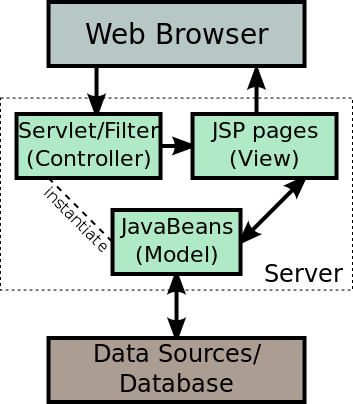
\includegraphics[scale=0.5]{./GoogleAppEngine/imagenes/JSP_Model.png}
  \caption{Modo de interpretación de un archivo JSP}
  \label{fig:modoJSP}
\end{figure}

Un fichero \textit{*.jsp} es la unión de código HTML con código java, el cual es interpretado en el momento de visualización de la página web. Un ejemplo es el siguiente:
 
\begin{lstlisting}[language=HTML]   
<!DOCTYPE html>
<html>
<body>
<table>
<tr>
	<th>ID</th>
	<th>Num sec</th>
	<th>Token de tiempo</th>
	<th>Mensaje</th>
	<th>URL para ver la firma</th>
	<th>Fecha</th>
	<th>Usuario</th>
	<th id="filadestino">Destino</th>
	<th>Verificado?</th>
</tr>

<% for (RowRepositorioGeneral row : rows) {%>
<tr>
	<td><%=row.getId()%></td>
	<td><%= row.getNum_sec()%></td>
	<td><%=row.getToken_tiempo()%></td>
	<td><%=row.getTexto_claro()%></td>
	<td><a href=<%=row.getUrl_firma()%>>URL para ver el token
			de tiempo</a></td>
	<td><%=row.getFecha()%></td>
	<td><%=row.getUsuario()%></td>
	<td id="filadestino"><%=row.getDestino()%></td>
	<td>
		<%
		Boolean confirmado = row.getConfirmado();
		if (!(confirmado == null) && confirmado) {
		%>
		<center>
			<img src="ok.png" />
		</center> <%} else  %>
	</td>
</tr>
<%}%>
</table>
</body>
</html>
\end{lstlisting}

Como se puede ver en este trozo de código este jsp genera una tabla que se rellena dinámicamente con los valores que devuelve un objeto java, se puede observar que se entrelazan trozos de código Java con etiquetas HTML. Si mostramos esta web y acto seguido introducimos otro objeto RowRepositorioGeneral en la estructura, cuando recarguemos la tabla tendrá una fila nueva.

\subsection{La carpeta WAR.}
La carpeta WAR es la carpeta principal para el despliegue de una aplicación web, ya que en ella es donde tienen que ir todos los archivos que necesitemos, desde archivos HTML, CSS, JSP, imágenes, etc. En la figura~\ref{fig:carpetawar} se puede ver un ejemplo de la carpeta WAR de mi aplicación web.

\begin{figure}
  \centering
    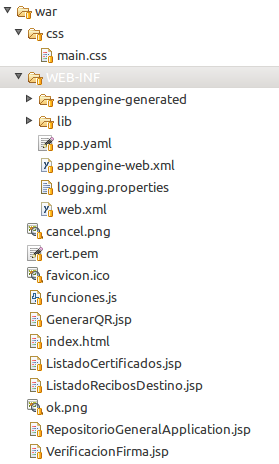
\includegraphics{./GoogleAppEngine/imagenes/carpetawar.png}
  \caption{Carpeta WAR}
  \label{fig:carpetawar}
\end{figure}

Se puede ver las diferentes carpetas y ficheros que la forman. Se ve la carpeta css que contiene los archivos de estilo que la página web usará, también se pueden ver los archivos \textit{web.xml} y \textit{app.yalm} que son archivos de configuración del servidor que se verán en el proximo apartado~\ref{ref_archivos_configuracion_google_app_engine} y además los archivos \textit{jsp} que se usan en la aplicación junto con los archivos \textit{html} y \textit{javascript} que se necesiten.

\subsection{Archivos de configuración.\label{ref_archivos_configuracion_google_app_engine}}
Los principales archivos de configuración son \textit{web.xml} y \textit{app.yalm}, este segundo es solo una forma de escribir de forma más legible el xml, para que nos sea más sencillo escribirlo y leerlo a los humanos.

Un ejemplo de un archivo \textit{web.xml} es el siguiente:

\begin{lstlisting}[language=XML]
<?xml version="1.0" encoding="utf-8"?>
<web-app xmlns:xsi="http://www.w3.org/2001/XMLSchema-instance"
xmlns="http://java.sun.com/xml/ns/javaee"
xmlns:web="http://java.sun.com/xml/ns/javaee/web-app_2_5.xsd"
xsi:schemaLocation="http://java.sun.com/xml/ns/javaee
http://java.sun.com/xml/ns/javaee/web-app_2_5.xsd" version="2.5">

	<servlet>
		<servlet-name>AddRow</servlet-name>
		<servlet-class>pfc.ServletCreateRow</servlet-class>
	</servlet>
	<servlet-mapping>
		<servlet-name>AddRow</servlet-name>
		<url-pattern>/add</url-pattern>
	</servlet-mapping>

	<welcome-file-list>
		<welcome-file>ServerTimestampApplication.jsp</welcome-file>
	</welcome-file-list>
</web-app>
\end{lstlisting}
%TODO: poner la referencia al código si se puede
Como se puede observar en el código se ha definido un servlet que se llamará \textbf{AddRow} que usará la clase \textbf{ServletCreateRow} y que estará mapeado en la dirección web \textbf{/add}, también podemos observar que el fichero que nos mostrará el servidor será \textbf{ServerTimestampApplication.jsp} si entramos a la url principal.

A continuación veremos como es un archivo \textit{app.yalm}:
\begin{lstlisting}[language=YAML]
application: repositoriorecibos
version: 1
runtime: java

handlers:
  - url: /add
    servlet: pfc.ServletCreateRow
    secure: always
welcome_files:
  - RepositorioGeneralApplication.jsp
\end{lstlisting}

Como podemos observar es mucho más fácil de entender y de escribir, el único problema que tienen los archivos YALM es que son sensibles a los espacios en blanco y tabuladores, por lo que hay que tener cuidado al redactarlos. En este archivo se crea un servlet en la ruta \textbf{/add}, que es la clase java \textbf{ServletCreateRow} del paquete \textbf{pfc} y que siempre hay que estar registrado en la aplicación para poder acceder a él. También podemos observar el fichero de bienvenida para cuando accedemos a la aplicación web. 
Al tener el archivo \textit{app.yalm} en la carpeta WEB-INF el parseador de YALM interpreta dicho archivo y genera un archivo \textit{web.xml} que es el que usará el servidor web para su configuración automáticamente.
\\
\\
Para ver todas las opciones de configuración que se pueden modificar en \textit{app.yalm} o en \textit{web.xml} se puede consultar estos enlaces \url{https://developers.google.com/appengine/docs/java/config/}, \url{https://developers.google.com/appengine/docs/java/configyaml/}. En el primero podemos ver todas las opciones configurables de \textit{web.xml} y el la segunda las de \textit{app.yalm}.

\section{Servidor de timestamp.}
En este apartado voy a explicar en profundidad todo lo relacionado con la aplicación de timestamp que he tenido que desarrollar, desde el diseño que se ha seguido hasta los problemas que me han surgido.

En principio me gustaría explicar para que se usa un servidor de timestamp en general. Un servidor de timestamp es un registro donde toda persona puede subir un documento y el servidor guarda ese documento añadiendole la fecha en la que se realizó la subida, dicha aplicación luego ofrece el servicio de consultar a que hora fue subido dicho documento. Un ejemplo podría ser \url{https://seguro.ips.es/servidortimestamp/index.asp} que se puede ver una captura de pantalla en la figura~\ref{fig:server_ips_timestamp}. En dicha captura podemos ver que tiene las opciones básicas de un servidor de timestamping como puede ser generar un sello, consultar su validez, etc. 

\begin{figure}[hbt]
  \centering
    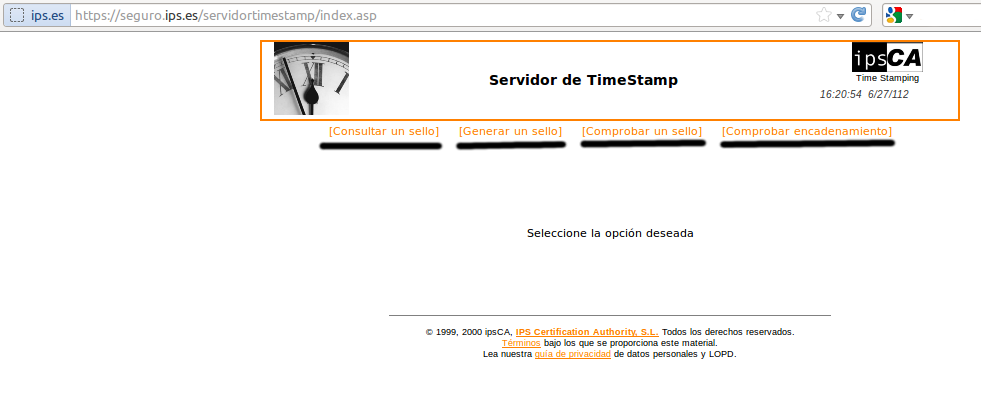
\includegraphics[scale=0.5]{./GoogleAppEngine/imagenes/server_ips_timestamp.png}
  \caption{Servidor Timestamp https://seguro.ips.es}
  \label{fig:server_ips_timestamp}
\end{figure}

La veracidad de que el sellado de dicho documento fue en el instante que dice ser, depende de la confianza que se tenga en ese servicio. Es similar a cuando se necesita que te sellen un documento físico, que dependiendo de para quien lo necesite, necesitas que lo firme un notario o un empleado público si es para una entidad pública. Normalmente suelen existir servidores de timestamping en los que se tiene confianza y los documentos sellados se consideran verdaderos.

Existen tres modelos principales de servidor de timestamping que son los siguientes:
\begin{itemize}
\item \textbf{Solución Arbitrada básica:} En esta solución el usuario que quiere sellar algo mandaría una copia del documento que quiere sellar a la entidad de sellado, que a su vez pondría el sello de tiempo y a su vez guardaría una copia de dicho documento, este es el modelo mas parecido a la vida real. Esta solución tiene un par de problemas grandes como puede ser que la privacidad del documento se pierde, tenemos que tener en cuenta que el servidor de timestamping puede estar en España, EEUU o en cualquier otro país y a su vez la base de datos para almacenar todos los documentos tiene que ser enorme, por lo que almacenar todos los documentos nos puede acarrear muchos problemas.

\item \textbf{Solución Arbitrada avanzada:} Esta solución es una evolución de la anterior, en ella el cambio que se hace es que el usuario que quiere que le sellen el documento manda el hash de dicho documento, un hash es el resultado de una función unidireccional que recibe un documento y devuelve un valor único, teniendo dicho valor no se puede saber el documento original, pero dicho documento siempre creará ese valor único, y la entidad solo tendría que almacenar dicho hash junto con el sello de tiempo que se ha generado. Esta solución no tiene los inconvenientes de la anterior, ya que el tamaño de los documentos se reduciría a unos pocos bytes, y la privacidad del documento no se ve comprometida. El problema que si persiste es que el usuario conozca a la entidad de certificación y puedan generar timestamp falsos, pero este problema ya va dentro de la confianza que queramos darle a ese servicio. Suponemos que si es un servicio oficial y serio este problema no va a suceder, de todas formas existen otras soluciones que arreglan este problema.

\item \textbf{Solución Arbitrada avanzada y distribuida:} Esta forma consigue arreglar el problema de la anterior que se produzca un uso fraudulento del timestamping es usando varias entidades de timestamping, por lo que el usuario mandaría el hash a varias entidades de sellado y el usuario guarde los reguardos que están firmados digitalmente de todas las entidades. Así si en una hay un problema tiene varias copias que certifican que se selló dicho instante.

\item \textbf{Solución mediante enlaces:} Esta solución es la mas compleja y a su vez la que soluciona todos los problemas anteriores, además tiene la ventaja de que no tiene que usar multitud de entidades de certificación. Consiste en que cuando un usuario quiere sellar algo, manda el hash del documento, la entidad añade el número de serie del documento anterior, el timestamp y lo firma digitalmente, entonces el problema de que se introduzcan valores fraudulentos por mitad se anula, ya que cada recibo está enlazado con el anterior.
\end{itemize}

En nuestro caso hemos desarrollado un servidor de timestamping en su versión solución arbitrada avanzada.

A continuación voy a explicar la aplicación web, los servlets que la componen y sus funciones.

\subsection{Explicación de la aplicación web.}
%TODO: falta explicar como funciona la BD...
En este capítulo voy a explicar todas las partes que componen la aplicación web que he desarrollado para la implementación del servidor timestamp.

En la figura~\ref{fig:paquete_pfc} se puede ver las clases que forman el paquete \textit{pfc}.

\begin{figure}
  \centering
    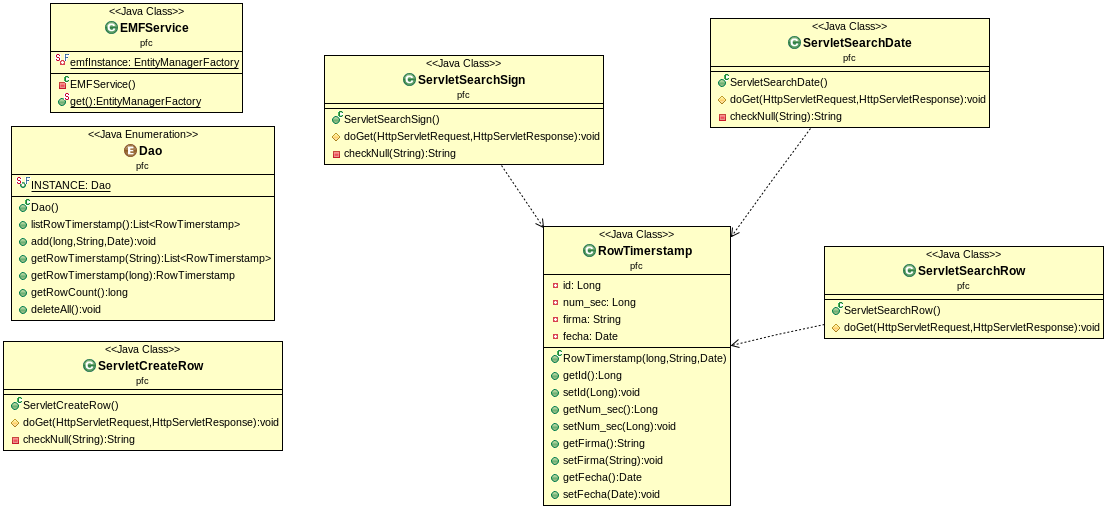
\includegraphics[scale=0.5]{./GoogleAppEngine/imagenes/UML_pfc.png}
  \caption{Detalles del paquete pfc}
  \label{fig:paquete_pfc}
\end{figure}

A continuación voy a explicar una a una las clases desarrolladas.

\begin{description}
\item \textbf{Dao.java: \label{prueba}} Esta clase es la encargada de todos los accesos a la base de datos, desde insercción, borrado y listado de las filas, hasta consultas que se necesiten hacer. Se puede observar que las consultas que son de listado de columnas se ejecutan con una sentencia SQL, un ejemplo es la siguiente:
\begin{lstlisting}[language=Java]
EntityManager em = EMFService.get().createEntityManager();
Query q = em.createQuery("select t from RowTimerstamp t where t.num_sec = :num_sec");
q.setParameter("num_sec", id);
RowTimerstamp RowTimerstamps = (RowTimerstamp)q.getSingleResult();
\end{lstlisting}

Pero las consultas que implican borrado o inclusión de filas no se realizan con sentencias SQL convencionales, se añaden con métodos que proporciona la API, un ejemplo es el siguiente:
\begin{lstlisting}[language=Java]
EntityManager em = EMFService.get().createEntityManager();
RowTimerstamp RowTimerstamp = new RowTimerstamp(num_sec, firma, fecha);
em.persist(RowTimerstamp);
em.close();
\end{lstlisting}

\item \textbf{RowTimerstamp.java:} En esta clase se diseña el formato de las filas de la base de datos, que como se ha explicado anteriormente no se crea con sentencias SQL, se usa un modelo de programación llamado JPA. Para dicho modelo hay que crear una clase que contenga como variables de clase las columnas de la tabla de la base de datos. Como podemos ver mediante anotaciones Java se le indica que campo es la clave primaría, también se puede indicar que ese campo es autoincrementado y otras opciones que habría que indicar en la creación de la tabla.   

\begin{lstlisting}[language=Java]
@Id
@GeneratedValue(strategy = GenerationType.SEQUENCE)
private Long id;
private Long num_sec;
private String firma;
private Date fecha;
\end{lstlisting}

Se puede ver que el campo id será la clave primaría que se indica con \textit{@id} y que es autoincremental, a su vez también podemos ver el resto de datos que se van a guardar, el campo \textit{num\_sec} es el número de secuencia, ya que el campo \textit{@id} lo usa la base de datos para organizarse ella, el campo \textit{firma} es hash firmado por el usuario y que se quiere tener constancia de que se subío en la fecha que indica el campo \textit{fecha}.
El resto de métodos que tiene esta clase es un contructor, getter para consultar los campos y setter para insertar valores.

\item \textbf{ServletCreateRow.java:} Esta clase es un servet que se encagar de recibir todos los parámetros necesarios y añadirlos a la base de datos. Al recibir los parámetros mediante \textbf{GET} tiene que implementar el método \textit{doGet}, casi todos los servlets implementados en el proyecto mandan los parámetros mediante \textbf{GET}. La forma de recibir parámetros es la siguiente:

\begin{lstlisting}[language=Java]
String firma = req.getParameter("firma");
\end{lstlisting}

El resto de parámetros que se necesitan se generan en el servidor para que no puedan ser falseados, como es el número de secuencia y la fecha.

Si la insercción se produce correctamente se devuelve una cadena que tiene el siguiente formato: ``ok;;num\_sec;;fecha" que será interpretado en la aplicación android y que parseará dicha cadena para conseguir los valores que necesitemos.

\item \textbf{ServletDeleteAll.java:} Es un servlet ``secreto" que se usa para borrar todas las filas del servidor, cosa que no se debería poder para no poder falsear los datos introducidos en el servidor de timestamp. Hay que llamarlo con un parámetro que es \textbf{borrar} con valor \textbf{5}.

\item \textbf{ServletSearchDate.java:} Es un servlet que devuelve una cadena con la fecha de una fila que tiene el número de secuencia que se le pasa en el parámetro \textbf{token}.

\item \textbf{ServletSearchRow.java:} Es un servlet que devuelve una página web donde se puede observar en una única columna toda la infomación almacenada que corresponde con el número de secuencia que se le pasa en el parámetro \textbf{id}. La forma de hacerlo es la siguiente:

\begin{lstlisting}[language=Java]
PrintWriter pw = resp.getWriter();
pw.print("<!DOCTYPE html>");
pw.print("<html><head><title>Lista Time Stamp</title><link rel=\"stylesheet\" type=\"text/css\" " +
		"href=\"css/main.css\"/> <meta charset=\"utf-8\"> </head>");
pw.print("<body><table><tr><th>ID</th><th>Num sec</th><th>Firma</th><th>Date</th></tr><tr> " +
		"<td>"+ row.getId() +"</td><td>"+ row.getNum_sec() +"</td><td>"+ row.getFirma() +"</td><td>" +
		row.getFecha() + "</td></tr> </table></body>");
pw.flush();
\end{lstlisting}

Como se puede ver se crea una tabla en una web que su fila se generan dinámicamente dependiendo del número de secuencia que se le pase.

\item \textbf{ServletSearchSign.java:} Es un servlet que devuelve una cadena con la firma que corresponde al número de secuencia que se pasa por el parámetro \textbf{token}.
\end{description}
%TODO: falta los jsp

\section{Servidor de registro de firmas.}
El servidor de registro de firmas que hemos desarrollado es una aplicación web en la que se pueden consultar las firmas que tu has realizado, las firmas en las que el destinatario eres tú, gestión del certificado de clave pública, verificar una firma, exportar una cadena con la que cualquier persona puede mirar si la firma que has realizado es válida para comprobaciones en caso de algún problema, y generar códigos QR para que que alguien que lo necesite pueda firmarlo.

El sistema de gestión de usuarios la proporciona google, y para entrar en la aplicación web hay que tener una cuenta de google, si no se produce una redirección a la página de logueo que se puede ver en la figura~\ref{fig:logueoRepoGeneral}.
\begin{figure}
  \centering
    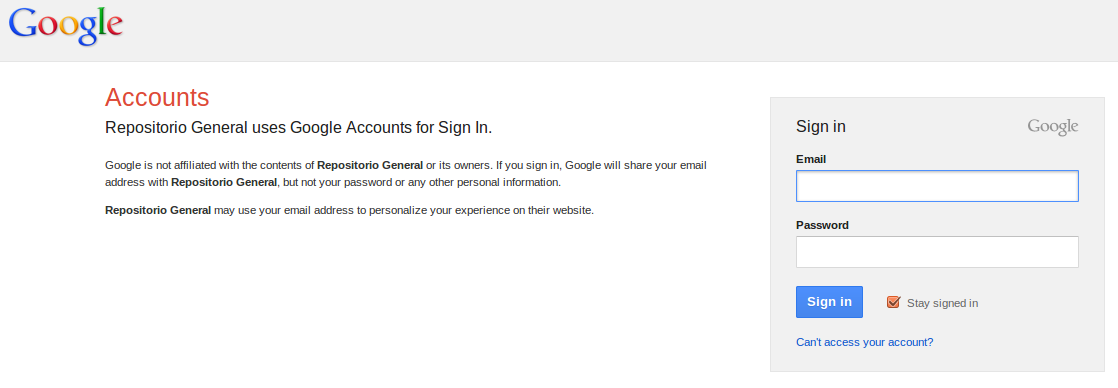
\includegraphics[scale=0.5]{./GoogleAppEngine/imagenes/login_repositorio_general.png}
  \caption{Login en Repositorio General}
  \label{fig:logueoRepoGeneral}
\end{figure}
La parte de la seguridad de los usuarios, logueo y mantenimiento de las base de datos ya las proporciona el mismo Google.

La aplicación web se puede ver en la figura~\ref{fig:repositorio_general}.
\begin{figure}[gae]
  \centering
    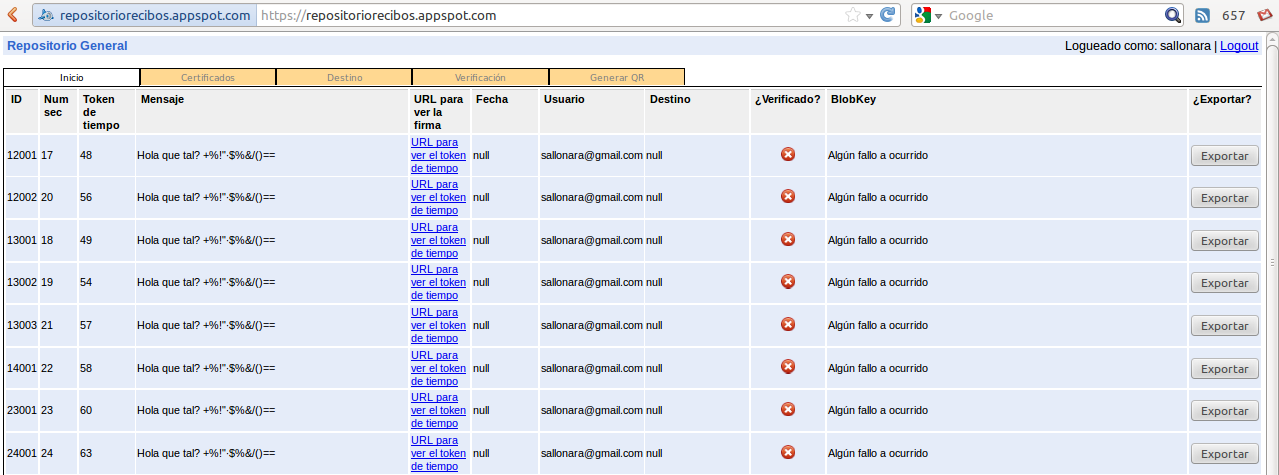
\includegraphics[scale=0.5]{./GoogleAppEngine/imagenes/repositorio_general.png}
  \caption{Repositorio General}
  \label{fig:repositorio_general}
\end{figure}

La aplicación tiene varias pestañas, que se explicarán posteriormente cuando expliquemos cada archivo \textit{*.jsp}, pero principalmente cada una de ellas se encarga de hacer una de las funciones que hemos comentado anteriormente.

\subsection{Explicación de la aplicación web.}
%TODO: falta explicar como funciona la BD...
En la figura~\ref{fig:clasesReposotorioGeneral} se puede ver las clases que forman el paquete \textit{pfc} de la aplicación web repositorio general.

\begin{figure}

    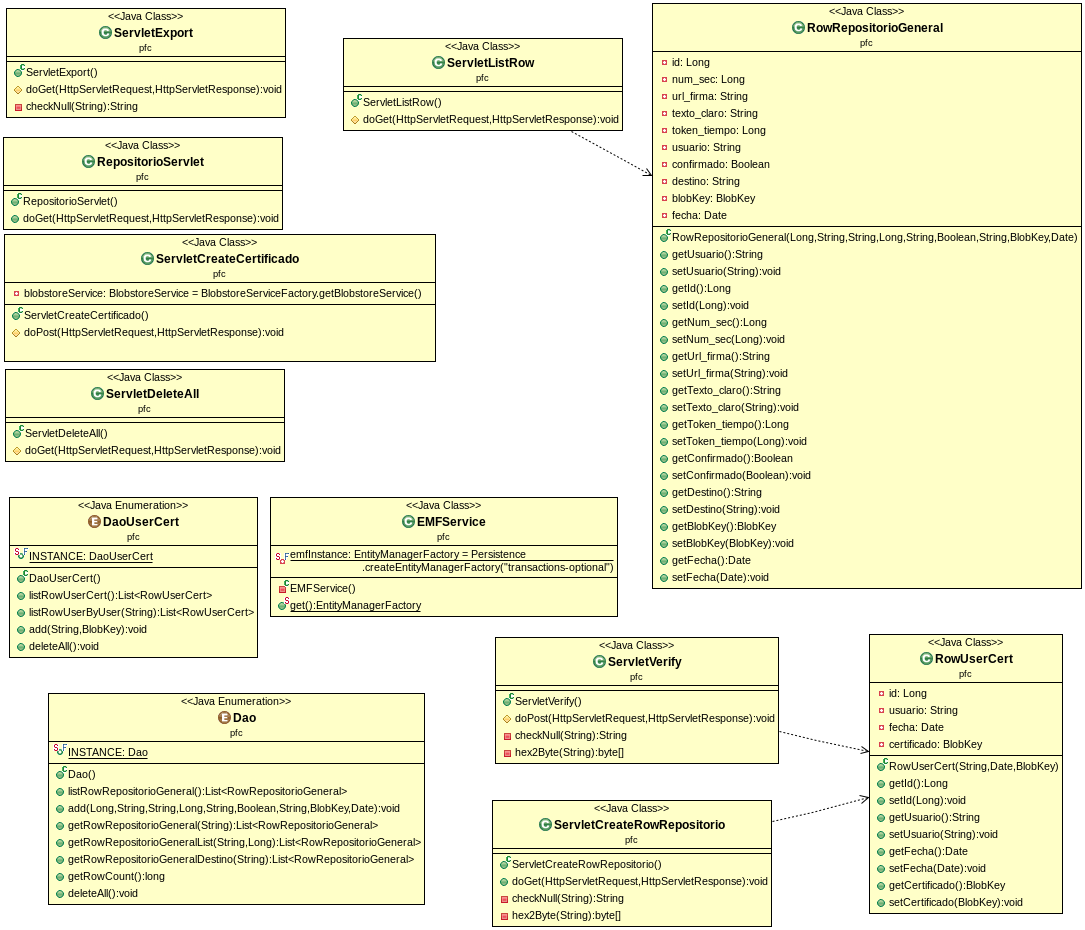
\includegraphics[scale=0.5]{./GoogleAppEngine/imagenes/UML_repositorio.png}
  \caption{Detalles de las clases Repositorio General.}
  \label{fig:clasesReposotorioGeneral}
\end{figure}

A continuación vamos a explicar una a una las clases desarrolladas.

\begin{description}
\item \textbf{Dao.java:} Al igual en el servidor de timestamp esta clase es la encargada de hacer todas operaciones contra la base de datos. Para mas información mirar el apartado~\ref{prueba}.

\item \textbf{DaoUserCert.java:} En este aplicación hemos utilizado dos bases de datos, una para guardar las firmas y otra para guardar los certificados de clave pública que se necesitan para verificar si una firma es correcta o no. Esta clase es la encargada de todos los accesos, tanto inserciones como consultas, a dicha tabla. 

\item \textbf{RowRepositorioGeneral.java:} Esta es la clase con la que se crea la tabla en la que se almacenan las firmas de los usuario, tiene los siguientes campos:  

\begin{lstlisting}[language=Java]
@Id
@GeneratedValue(strategy = GenerationType.SEQUENCE) //	 GenerationType.IDENTITY
private Long id;
private Long num_sec;
private String url_firma;
private String texto_claro;
private Long token_tiempo;
private String usuario;
private Boolean confirmado;
private String destino;
private BlobKey blobKey;
private Date fecha;
\end{lstlisting}

Tiene una clave primaría que es \textit{id} que es usada por Google internamente para el almacenado de la información, \textit{num\_sec} es el número de secuencia dentro la tabla que va incrementandose automáticamente, \textit{url\_firma} es la dirección en la cual se puede consultar la firma del texto en claro que está en el campo \textit{texto\_claro}. También se guarda el \textit{token\_tiempo} que es el \textit{num\_sec} de en la aplicación web del servidor de timestamp. La columna \textit{usuario} almacena el usuario que ha subido la firma, y en La columna \textit{destino} se guarda a quien va dirigido la firma, ya que todas firmas tienen un destinatario. En la columna \textit{blobkey} se guarda la referencia al certificado de clave pública que estaba en activo cuando fue subido a la aplicación web, la columna \textit{confirmado} puede valer true or false e indica si al subir la firma se pudo verificar y el texto en claro coincidía con el texto cifrado, en \textit{fecha} está la fecha en la que se almacenó.

\item \textbf{RowUserCert.java:} Esta clase es la encagargada de crear la tabla que usamos para guardar los archivos con la clave pública.
%TODO: poner el tipo de archivo que necesitamos usar y esas cosas.
Los campos que usaremos para almacenarlos serán los que se pueden ver en 

\begin{lstlisting}[language=Java]
@Id
@GeneratedValue(strategy = GenerationType.SEQUENCE)
private Long id;
private String usuario;
private Date fecha;
private BlobKey certificado;
\end{lstlisting}

Como podemos observar el campo \textit{id} será la clave pública y como hemos explicado será usado por la base de datos de Google para autogestión de las filas, el campo \textit{usuario} guardará una cadena con el email de la persona que ha subido ese archivo, el campo \textit{fecha} es la fecha en la que se subió el archivo, dicho campo se usará para comprobar que no se puedan falsear firmas, con varias comprobaciones y para anular certificados en caso de perdidas o que se necesite reemplazarlo, \textit{certificado} es un campo del tipo \textbf{BlobKey} que es como la ruta al archivo de certificado.

\end{description}
A continuación vamos a explicar los diferentes servlets que hemos desarrollado para la aplicación web.

\begin{description}
\item \textbf{ServletCreateCertificate.java:} Este servlet es el encargado de añadir a la base de datos el certificado de clave pública. Es usado en la pestaña de certificados de la aplicación web y es llamado cuando se pulsa subir certificado. Se puede observar el botón subir certificado en la figura~\ref{fig:pestanhaCertificados}.

\begin{figure}
  \centering
    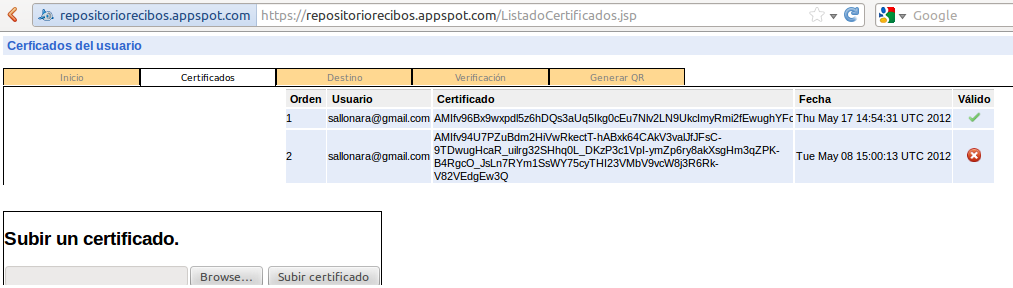
\includegraphics[scale=0.5]{./GoogleAppEngine/imagenes/certificadosRepositorioGeneral.png}
  \caption{Pantallazo de la pestaña certificados.}
  \label{fig:pestanhaCertificados}
\end{figure}

\item \textbf{ServletCreateRowRepositorio.java:} Este servlet está mapeado en la dirección: \url{https://repositoriorecibos.appspot.com/add} y recibe los siguientes parámetros: \textit{texto}, \textit{url\_firma}, \textit{token}, \textit{destino} y \textit{fecha}. Es el encargado de añadir una fila por cada llamada a dicha dirección, a dicho dirección no hay forma de acceder desde la aplicación web, solo se pueden comprobar las firmas ya introducidas. A su vez antes de introducir la fila comprueba que la firma se puede validar y marca como verdadero o falso la columna verificado que posteriormente en el archivo \textit{RepositorioGeneralApplication.jsp} se cambiará por una imagen para hacer la verificación más visual. Si se hemos podido insertar la fila, el servlet devuelve la cadena \textbf{OK}, si no se devuelven varias cadenas con los fallos que se han producido.

\item \textbf{ServletDeleteAll.java:} Servlet ``secreto" que borra todas las filas de firmas almacenadas, hay que llamarlo con un parámetro que es \textit{borrar} con valor \textit{7}

\item \textbf{ServletExport.java:} Este servlet es el encargado de exportar una fila de nuestras filas para que otra persona pueda comprobar si es válida. Este servlet es llamado cuando se pulsa el botón exportar de la pestaña principal de la aplicación web. Se puede observar en la figura~\ref{fig:botonExportar}

\begin{figure}
  \centering
    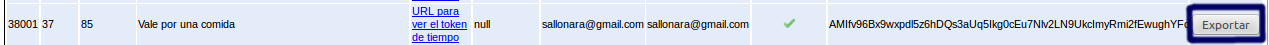
\includegraphics[scale=0.5]{./GoogleAppEngine/imagenes/botonExportar.png}
  \caption{Detalle del botón exportar.}
  \label{fig:botonExportar}
\end{figure}

El servlet recibe los siguiente parámetros:

\begin{lstlisting}[language=Java]
String mensaje = checkNull(req.getParameter("mensaje"));
String url_firma = checkNull(req.getParameter("token"));
String id_blob = checkNull(req.getParameter("id_blob"));
String user = checkNull(req.getParameter("usuario"));
\end{lstlisting}

Una vez se tienen esos parámetros creamos una cadena de texto en la que unimos los siguiente campos y cada parámetro va separado por el separador: \textit{;/:}.
\begin{lstlisting}[language=Java]
String cadACodificar = mensaje + ";/:" + url_firma + ";/:" + id_blob + ";/:" + user;
\end{lstlisting}

Acto seguido codificamos la cadena con \textbf{Base64}, que es una forma simple de codificar los caracteres para que no viajen en texto claro.
\begin{lstlisting}[language=Java]
String cadCodificada = Base64.encode(cadACodificar.getBytes("UTF-8"));
\end{lstlisting}

También añadimos unos limitadores para que cuando tengamos que decodificar ese mensaje podamos saber donde empiezan y donde termina la exportación.
\begin{lstlisting}[language=Java]
pw.println("BEGIN EXPORT");
pw.println("--------------------------");
pw.println(cadCodificada);
pw.println("--------------------------");
pw.println("END EXPORT");
\end{lstlisting}

\item \textbf{ServletListRow.java:} Este servlet es el encargado en devolver todas las filas de la tabla que pertenecen a un usuario. La forma de hacerlo es la siguiente, primero se identifica el usuario con el que se ha logueado de esta forma:

\begin{lstlisting}[language=Java]
UserService userService = UserServiceFactory.getUserService();
User user = userService.getCurrentUser();
\end{lstlisting}

Una vez se consigue el usuario se llama a la función \textit{public List<RowRepositorioGeneral> getRowRepositorioGeneralList(String userId, Long num\_sec)} de la clase \textit{Dao.java}, esta última función nos devuelve una lista con todas las filas. Al llamar al servlet le pasaremos el último número de secuencia que tenemos guardado en el telefono móvil, para así agilizar las transferencias de datos, de esta forma solo nos devolverá las filas nuevas. La forma de devolvernos las filas será en un JSONArray, que es un objeto que dentro tiene varios objetos JSON\footnote{Para saber que es un objeto JSON pueden consultar los siguientes enlaces:\url{http://www.json.org/} o \url{http://en.wikipedia.org/wiki/JSON}}.

La creación de los objetos JSON la realizamos de la siguiente forma:
\begin{lstlisting}[language=Java]
JSONObject jsonObject = new JSONObject();

jsonObject.put("num_sec", rowRepositorioGeneral.getNum_sec().toString());
jsonObject.put("texto", rowRepositorioGeneral.getTexto_claro());
jsonObject.put("url_firma", rowRepositorioGeneral.getUrl_firma());
jsonObject.put("token_tiempo", rowRepositorioGeneral.getToken_tiempo().toString());
jsonObject.put("usuario",rowRepositorioGeneral.getUsuario());
jsonObject.put("fecha", rowRepositorioGeneral.getFecha().toString());
jsonObject.put("verificado", rowRepositorioGeneral.getConfirmado().toString());
jsonObject.put("destino", rowRepositorioGeneral.getDestino());
\end{lstlisting}

Ese objeto JSON se añade un objeto JSONArray que a su vez es el que devolveremos como respuesta al final de la ejecución de nuestro servlet y que espera la aplicación android que lo ha pedido.

\item \textbf{ServletVerify.java:} Este servlet es el utilizado en la pestaña verificar de nuestra aplicación web, como se puede observar en la figura~\ref{fig:pestañaVerificar}

\begin{figure}

    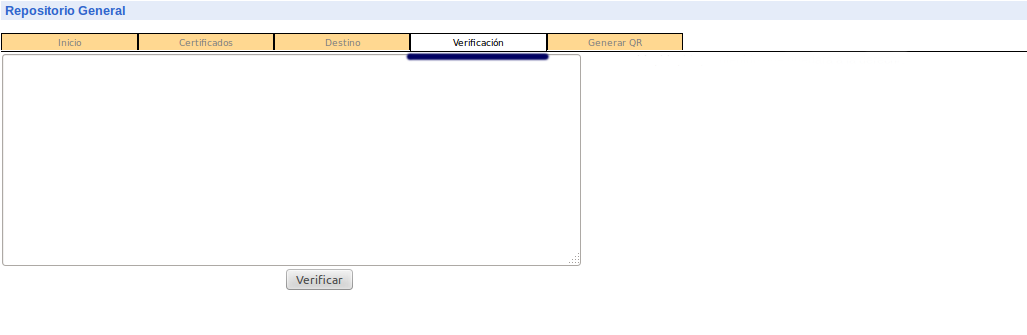
\includegraphics[scale=0.5]{./GoogleAppEngine/imagenes/pestanhaVerificar.png}
  \caption{Detalle de la pestaña verificación.}
  \label{fig:pestañaVerificar}
\end{figure}

Como podemos observar hay un cuadro de texto para introducir la cadena que devolvería al pulsar el botón exportar. Cualquier usuario puede verificar si una firma es correcta o no. En este servlet se hace el proceso contrario que hicimos en exportar, quitamos los indicadores de inicio y final de exportación, desencriptamos la cadena en Base64 y hacemos varias comprobaciones. Comprobamos que en la fecha en la que se firmó el certificado era válido y que no habiamos revocado ese certificado, también se comprueba que no fuera reemplazado por otro certificado antes de su expiración, ya que entonces la firma no sería válida. También comprobamos la integridad del mensaje, que la cadena no esté mal formada y que siga el formato que hemos obligado anteriormente.
\end{description}

Los archivos \textit{*.jsp} que hemos creado en su mayoría solo rellenan tablas dinámicamente haciendo llamadas a funciones de la clase \textit{Dao.java}. Solo habría uno que no realiza esas funciones que es el siguiente:
\begin{description}
\item \textbf{GenerarQR.jsp:} Este archivo JSP es el que se muestra en la pestaña \textit{Generar QR}, se puede ver en la figura~\ref{fig:pestanhaQR}. Su función es generar un código QR para que pueda ser leido por la aplicación del móvil. Hay que rellenar los campos de destino y el texto que queremos que firme dicha persona. Al darle a \textit{Generar código QR} se hace una llamada a la API Google Chart y se genera un código QR que contiene dichas cadenas y se muestra en la parte de la derecha, como se puede ver en la figura~\ref{fig:codigoQR}.

\begin{figure}
    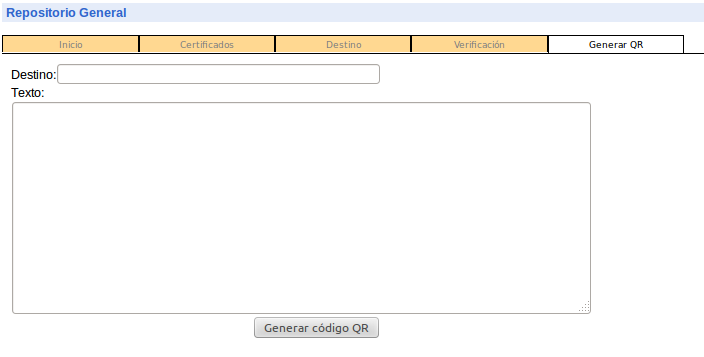
\includegraphics[scale=0.5]{./GoogleAppEngine/imagenes/pestanhaQR.png}
  \caption{Pestaña para generar el código QR.}
  \label{fig:pestanhaQR}
\end{figure}

\begin{figure}

    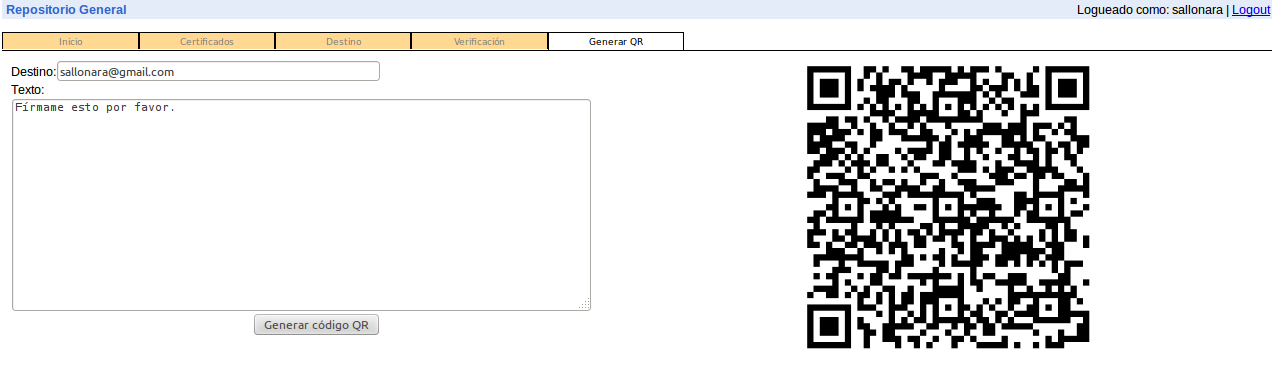
\includegraphics[scale=0.5]{./GoogleAppEngine/imagenes/codigoQR.png}
  \caption{Pestaña con el código QR generado.}
  \label{fig:codigoQR}
\end{figure}

\end{description}



	\appendix
	
	\backmatter
		\listoffigures
	
\end{document}
